\section{Background Contribution}\label{section:star_background}
The total background contribution to the charged-particle density can be broken down into
event-level and track-level backgrounds, which are described in detail in the following sections:
\begin{itemize}
	\item Accidental background refers to all classes of non-collision events which do not originate from a single collision of two protons from colliding bunches.
	\item Non-SD background comprise contibution of non-SD events which originate from a single $pp$ collision.
	\item Track backgrounds from non-primary tracks consist of secondary tracks and fake tracks; the first come mostly from decays, the short-lived particles with mean life $30 < \tau < 300$~ps, or secondary interactions with the detector dead material, while the second comes from the track reconstruction algorithms and out-of-time pile-up with
	no corresponding generated particles.
\end{itemize}
%accidentals
\section{Accidental Background}\label{section:star_accidentals}
The accidental backgrounds (same bunch pile-up background) are quantified using data-driven method and defined as a process where in  single bunch crossing there is coincidence of two interactions, where any single-side proton signal is collected in coincidence with a~signal in the~TPC-TOF detector. %This has the same signature as a signal process but would not come from a DD, a CD or a ND interaction. 
This type of background may come from the overlap of a~signal in \ac{RP} (proton from beamhalo, low mass \ac{SD} process without activity in TOF, elastic or low mass \ac{CD} processes with undetected proton on the other side) with a~signal in TPC+TOF (mainly \ac{ND} events without forward proton).

The accidental background contribution was calculated  from Zerobias data, where two signatures of such background were investigated: the reconstructed proton in RP and the reconstruction of vertex from TPC tracks matched with TOF. The analysis was done for each RP arm separately and thus the 
 Zerobias data was firstly required to pass the following criteria:
\begin{enumerate}
	\item no trigger in any RP or trigger in exactly one arm (two RPs) with exactly one reconstructed proton track in that arm,
	\item veto on any signal in small BBC tiles or ZDC on the same  side of the IP as  RP under consideration,
	\item no or exactly one reconstructed vertex with at least two TOF-matched tracks passing the quality criteria. The latter includes also signal in BBC small tiles on the opposite side of the IP to the RP under study. 
\end{enumerate}
 The sample of selected Zerobias data with total  number  of events $N$ was divided into four classes:
\begin{equation}
N=N(P,S)+N(R,S)+N(P,T)+N(R,T)
\label{eq:accidentalSTAR_N}
\end{equation}
where: $N(P,S)$ is the~number of events with reconstructed proton in exactly one RP and reconstructed TOF vertex, $N(R,S)$  is the~number of events with no trigger in any RP and reconstructed TOF vertex, $N(P,T)$ is the~number of events with reconstructed proton in exactly one RP and no reconstructed TOF vertex, $N(R,T)$ is the~number of events with no trigger in any RP and no reconstructed TOF vertex.\\

Since the signature of the signal is a reconstructed proton in exactly one RP and a~reconstructed TOF vertex, the number of such events can be expressed as:
\begin{equation}
N(P,S)=N\left(p_3+p_1p_2\right)
\end{equation}
where: $p_1$ is the~probability that there is a~reconstructed proton in RP and there is no reconstructed TOF vertex, $p_2$ is the~probability that there is no reconstructed proton in RP and  there is a~reconstructed TOF vertex, $p_3$ is the~probability that there is a~reconstructed proton in RP and  there is a~reconstructed TOF vertex (not accidental).

The other classes of events given in Eq.~\eqref{eq:accidentalSTAR_N} can be expressed in terms of the~above probabilities as:
\begin{equation}
\begin{split}
N(R,S)=  & N(1-p_1)p_2(1-p_3)\\
N(P,T) = & N(1-p_2)p_1(1-p_3)\\
N(R,T) = & N(1-p_1)(1-p_2)(1-p_3)
\end{split}
\end{equation}
Finally, the accidental background contribution $A_{\mathrm{bkg} }^{\mathrm{accidental}}$ is  given by:
\begin{equation}
\begin{split}
A_{\mathrm{bkg}}^{\mathrm{accidental}}=  \frac{p_1p_2}{p_3+p_1p_2}=\frac{N(R,S)N(P,T)N}{N(R)N(T)N(P,S)}
\end{split}
\label{eq:bkg_acc_norm}
\end{equation} 
where: $N(R)=N(R,S)+N(R,T)$ and $N(T)=N(P,T)+N(R,T)$.

The shapes of the accidental background related to TPC distributions come from the~above Zerobias data events which pass all the analysis selection except having no trigger in any RP. The~templates corresponding to RP distributions are from protons in the~above data sets but with no reconstructed TOF vertex. The normalization is given by Eq.~\eqref{eq:bkg_acc_norm}. Figure~\ref{fig:STARaccidentalsXi} shows distributions of the~reconstructed $\xi$ with the~accidental background contribution  for events with proton reconstructed in EU, ED, WU and WD arms. Accidental background in the~range of $0.02<\xi<0.2$ is below $1\%$.

\begin{figure}[h!]
	\centering
	\includegraphics[width=0.49\textwidth, page=40]{chapters/chrgSTAR/img/accidentals/accidentalBkg.pdf}
	\includegraphics[width=0.49\textwidth, page=41]{chapters/chrgSTAR/img/accidentals/accidentalBkg.pdf}
	\includegraphics[width=0.49\textwidth, page=42]{chapters/chrgSTAR/img/accidentals/accidentalBkg.pdf}
	\includegraphics[width=0.49\textwidth, page=43]{chapters/chrgSTAR/img/accidentals/accidentalBkg.pdf}
	\caption{Uncorrected distributions of the reconstructed $\xi$ for events with proton reconstructed in  (top left) EU, (top right) ED, (bottom left) WU and (bottom right) WD arms. Data is shown as black markers, whereas the~accidental background contribution is shown as yellow histogram.  The ratio of accidental background and data is shown in the bottom pad.}
	\label{fig:STARaccidentalsXi}
\end{figure}

The selection of Zerobias events, which is not unique, may provide some bias to the normalization of the~accidental background. As a systematic check, two criteria for  Zerobias selection were changed~to:
 \begin{enumerate}
 	\item no trigger in any RP or trigger in exactly one arm (two RPs) with \textit{no more} than one reconstructed proton track in that arm, i.e. events with trigger signals in exactly one arm and without reconstructed proton track in that arm were also used,
 	%\item veto on any signal in small BBC tiles or ZDC on the same  side of the IP as  RP under study,
 	\item no  or exactly one reconstructed TOF vertex (%not necessarily  with two TOF-matched tracks passing the quality criteria). 
 	\textit{without any additional requirements}), i.e. events with a~reconstructed TOF vertex that does not have at least two primary tracks satisfying the~selection criteria (Sec.~\ref{section:star_track_selection}), or with a~reconstructed TOF vertex that is out of the~range of $|V_z|<80$~cm, were also accepted. The requirement of signal in BBC small tiles remains unchanged. 
 \end{enumerate}
 As a result of this change in the procedure, %, as shown in Fig.~\ref{fig:STARaccidentalsXiSyst}, 
 the accidental background normalization increases of about $50\%$ with respect to the nominal value. Therefore, the background changes by $\pm50\%$ was taken as a systematic uncertainty related to the accidentals.
 
 \begin{comment}
 \begin{figure}[h!]
 	\centering
 	\includegraphics[width=0.49\textwidth, page=40]{chapters/chrgSTAR/img/accidentals/accidentalBkg_test.pdf}
 	\includegraphics[width=0.49\textwidth, page=41]{chapters/chrgSTAR/img/accidentals/accidentalBkg_test.pdf}
 	\includegraphics[width=0.49\textwidth, page=42]{chapters/chrgSTAR/img/accidentals/accidentalBkg_test.pdf}
 	\includegraphics[width=0.49\textwidth, page=43]{chapters/chrgSTAR/img/accidentals/accidentalBkg_test.pdf}
 	\caption{Uncorrected distributions of the reconstructed $\xi$ for events with proton reconstructed in (top left) EU, (top right) ED, (bottom left) WU and (bottom right) WD arms. The~accidental background contribution calculated with changed Zerobias selection criteria is also shown.}
 	\label{fig:STARaccidentalsXiSyst}
 \end{figure}
\end{comment}




%non-SD
% !TeX spellcheck = en_GB
\section{Control Plots}\label{section:star_nonSD}
\begin{comment}
The background contributions coming from \ac{ND}, \ac{DD} and \ac{CD} events are estimated from \ac{MC} simulations. Protons from elastic interactions and beam halo are not included in the~simulation. \ac{SD} background signatures which are modeled in th~\ac{MC} simulations are only coming from :
\begin{itemize}
\item forward protons produced in the \ac{SD}, \ac{CD} or \ac{DD} diffractive systems or through non-diffractive  \ac{QCD},
\item reconstructed tracks coming from showering.
\end{itemize}

Figure~\ref{fig:nonSDxit} shows the uncorrected $\xi$ and $t$ distributions in data compared to various \ac{MC} models: PYTHIA 8 A2 (MBR), PYTHIA 8 A2 (MBR-tuned) and EPOS. The \ac{MC} distributions are split into \ac{SD}, \ac{ND}, \ac{DD} and \ac{CD} components. For EPOS low mass excitation of the proton remnant (SD') is separated from the ND events. Additionally, the accidental background is also shown. Without arbitrary suppression of diffractive cross sections at large $\xi$ PYTHIA8 A2 (MBR-tuned) predictions agree much better with the data and result also in a suppression of non-SD events. EPOS describes data better than PYTHIA8 but shows a dominant contribution of SD' events. All MCs predict significant non-SD background at large $\xi$, thereby  the analysis was limited to $\xi < 0.2$. 

On the other hand, \cref{fig:nonSDnsel,fig:nonSDpt,fig:nonSDera} show the uncorrected distributions of variables used in the later analysis: $n_{\mathrm{sel}}$, $p_{\mathrm T}$ an $\bar{\eta}$. The background contributions from non-SD interactions differ a bit between each other, i.e. EPOS predicts significantly larger CD contribution, whereas DD and ND are suppressed in PYTHIA 8 A2 (MBR-tuned).  As a result PYTHIA~8~A2~(MBR) is used as the default model  of non-SD with systematic uncertainty $\pm50\%$, which covers all differences between the~models. %Moreover, SD' in EPOS was not subtracted but used separately for comparisons.

\begin{figure}[H]
\centering
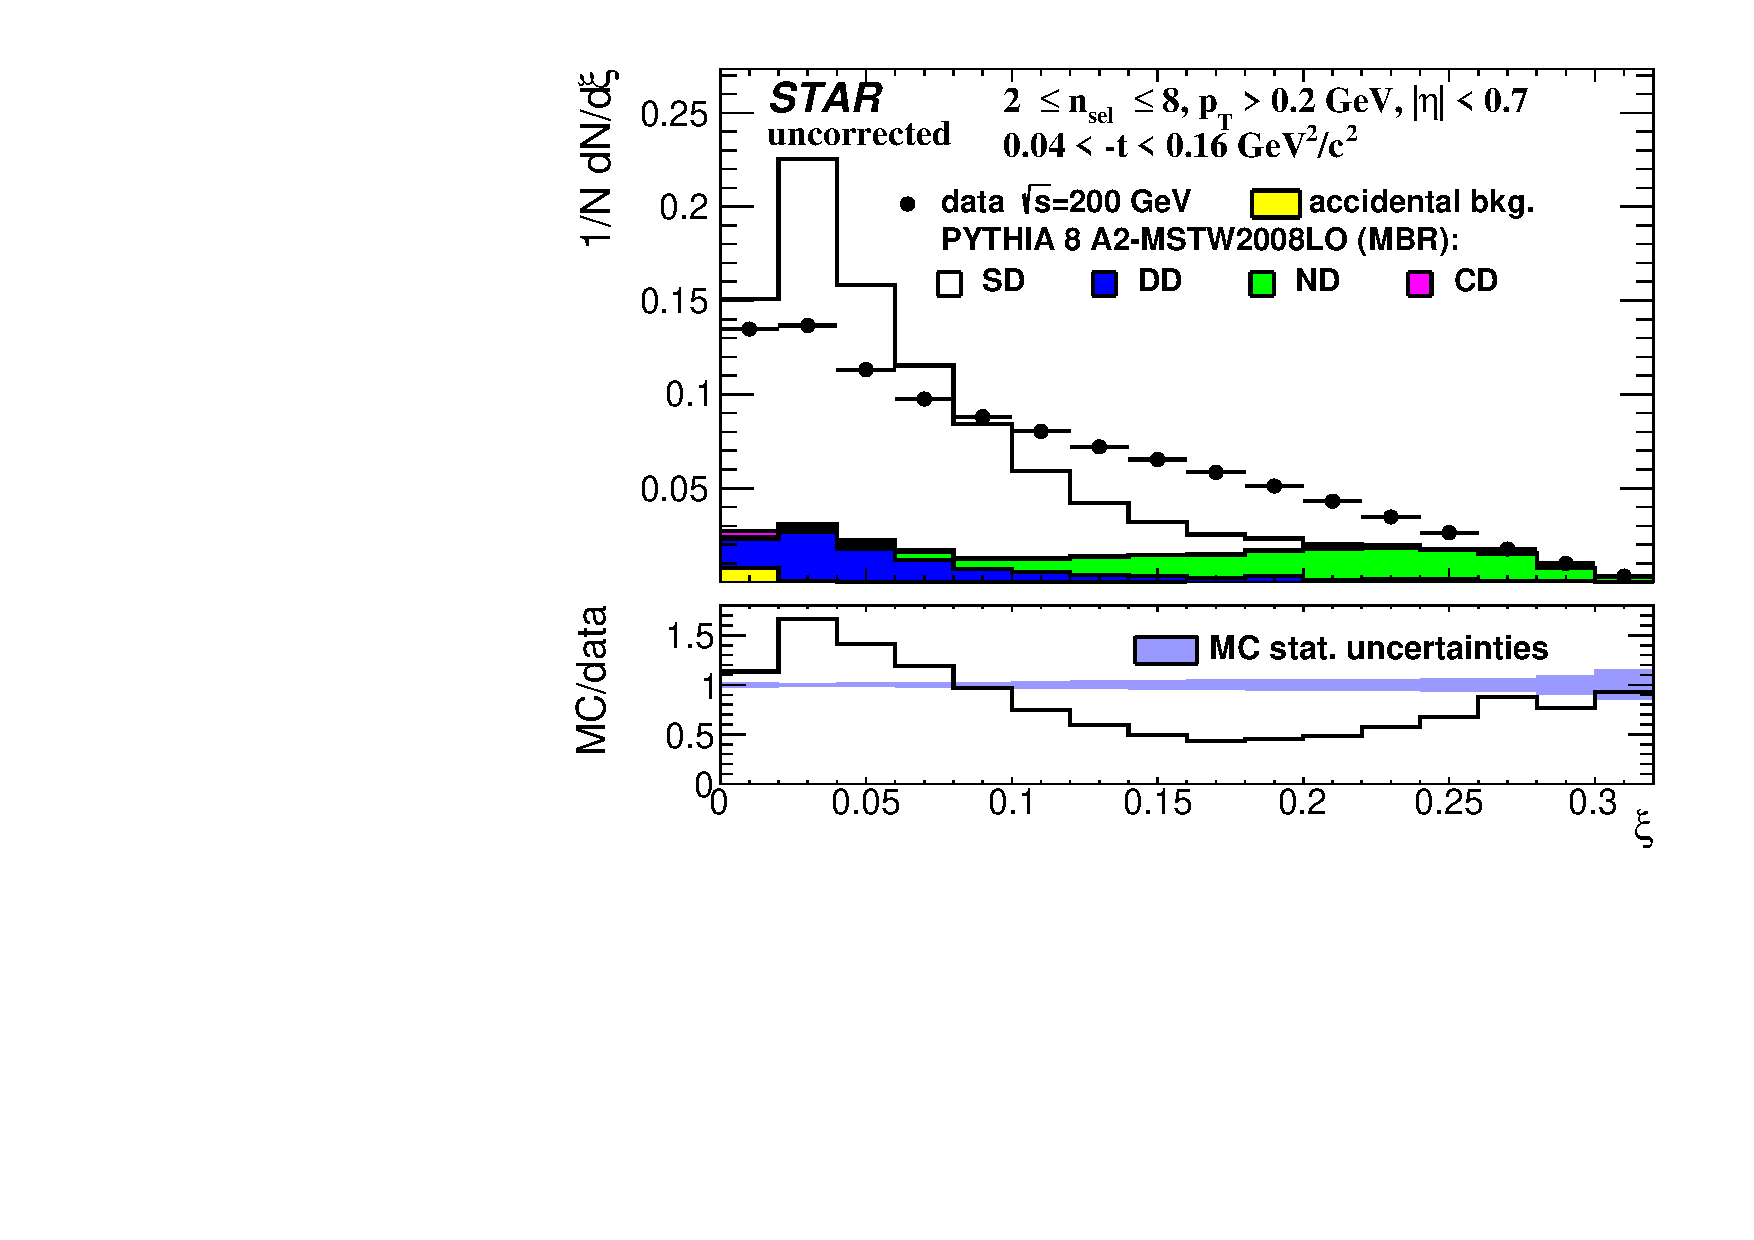
\includegraphics[width=.49\textwidth,page=1]{chapters/chrgSTAR/img/nonSD/SDT_pythia_xi0_RP_starsim_xi.pdf}
\hfill
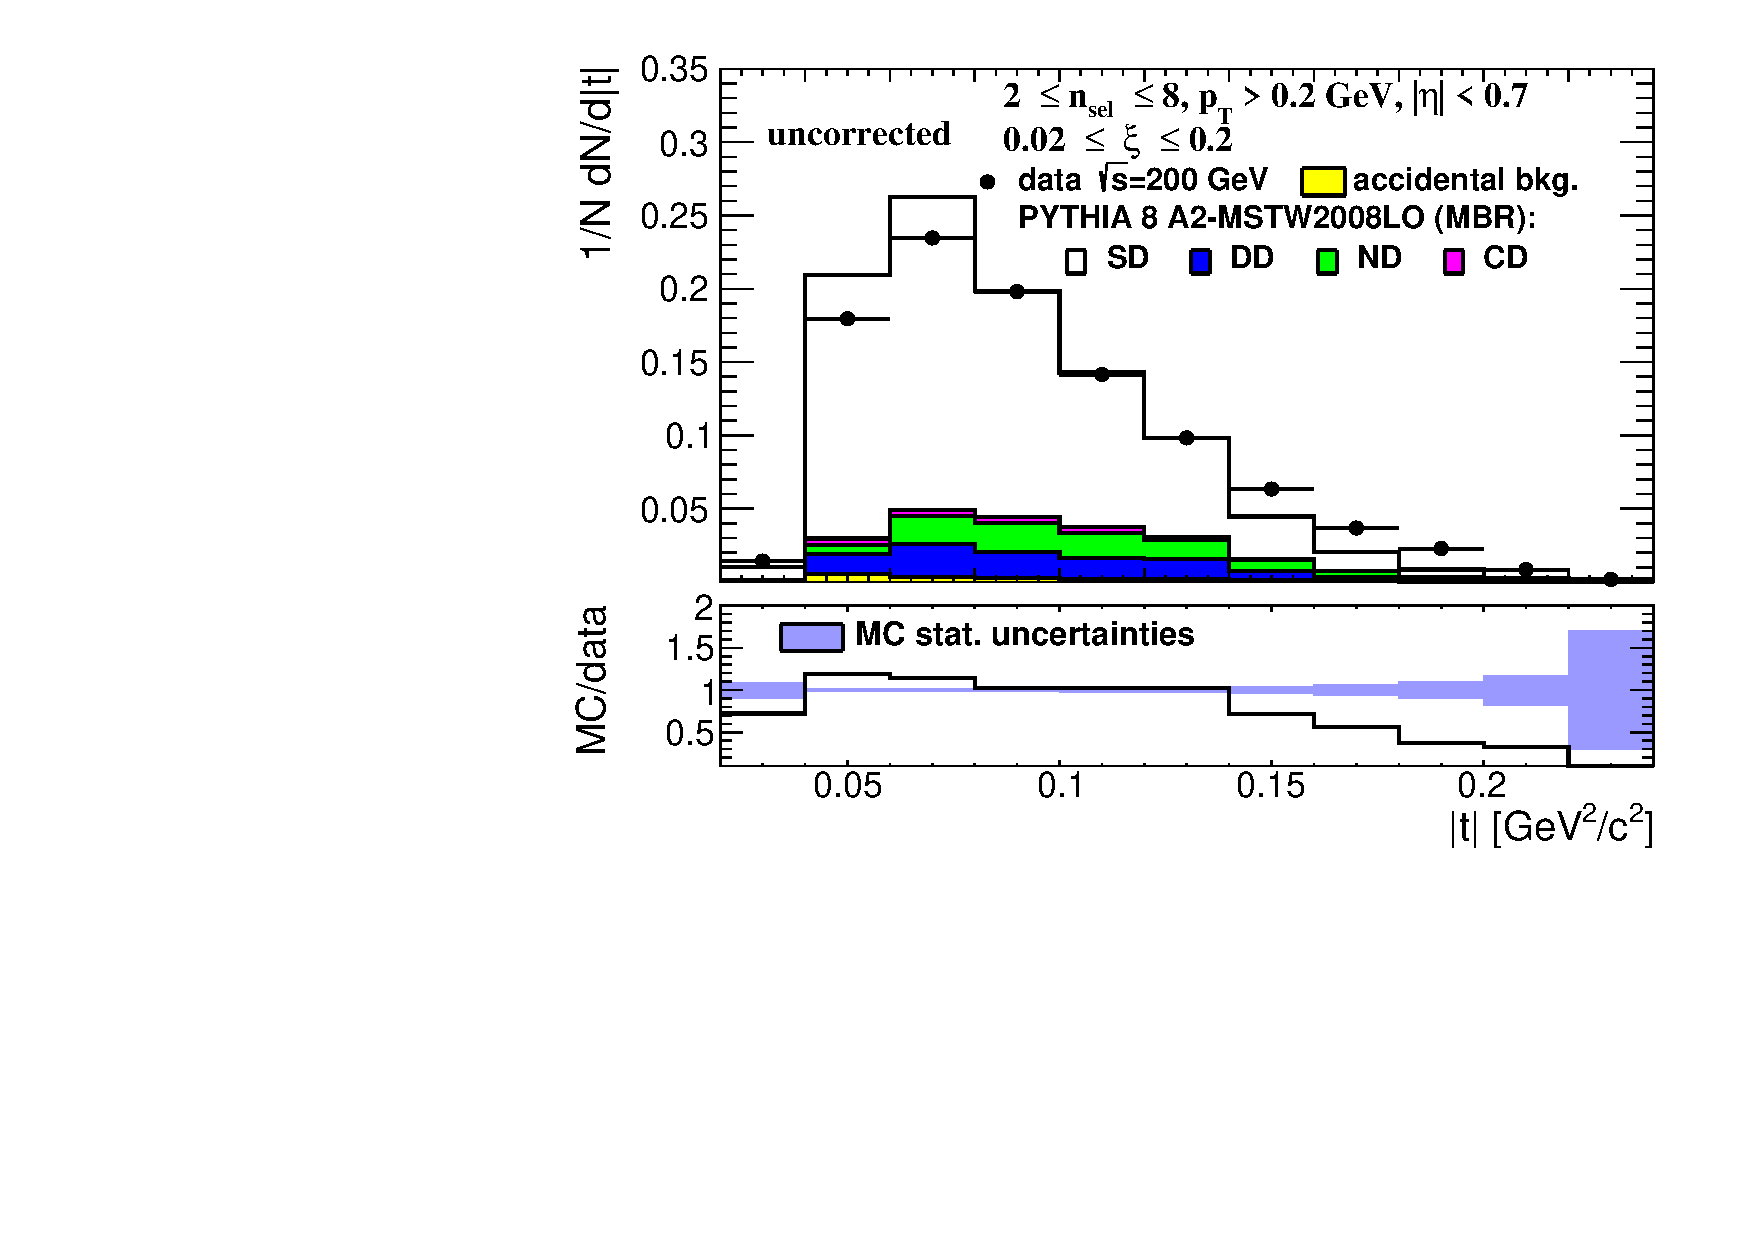
\includegraphics[width=.49\textwidth,page=1]{chapters/chrgSTAR/img/nonSD/SDT_pythia_xi0_RP_starsim_t.pdf}
\newline
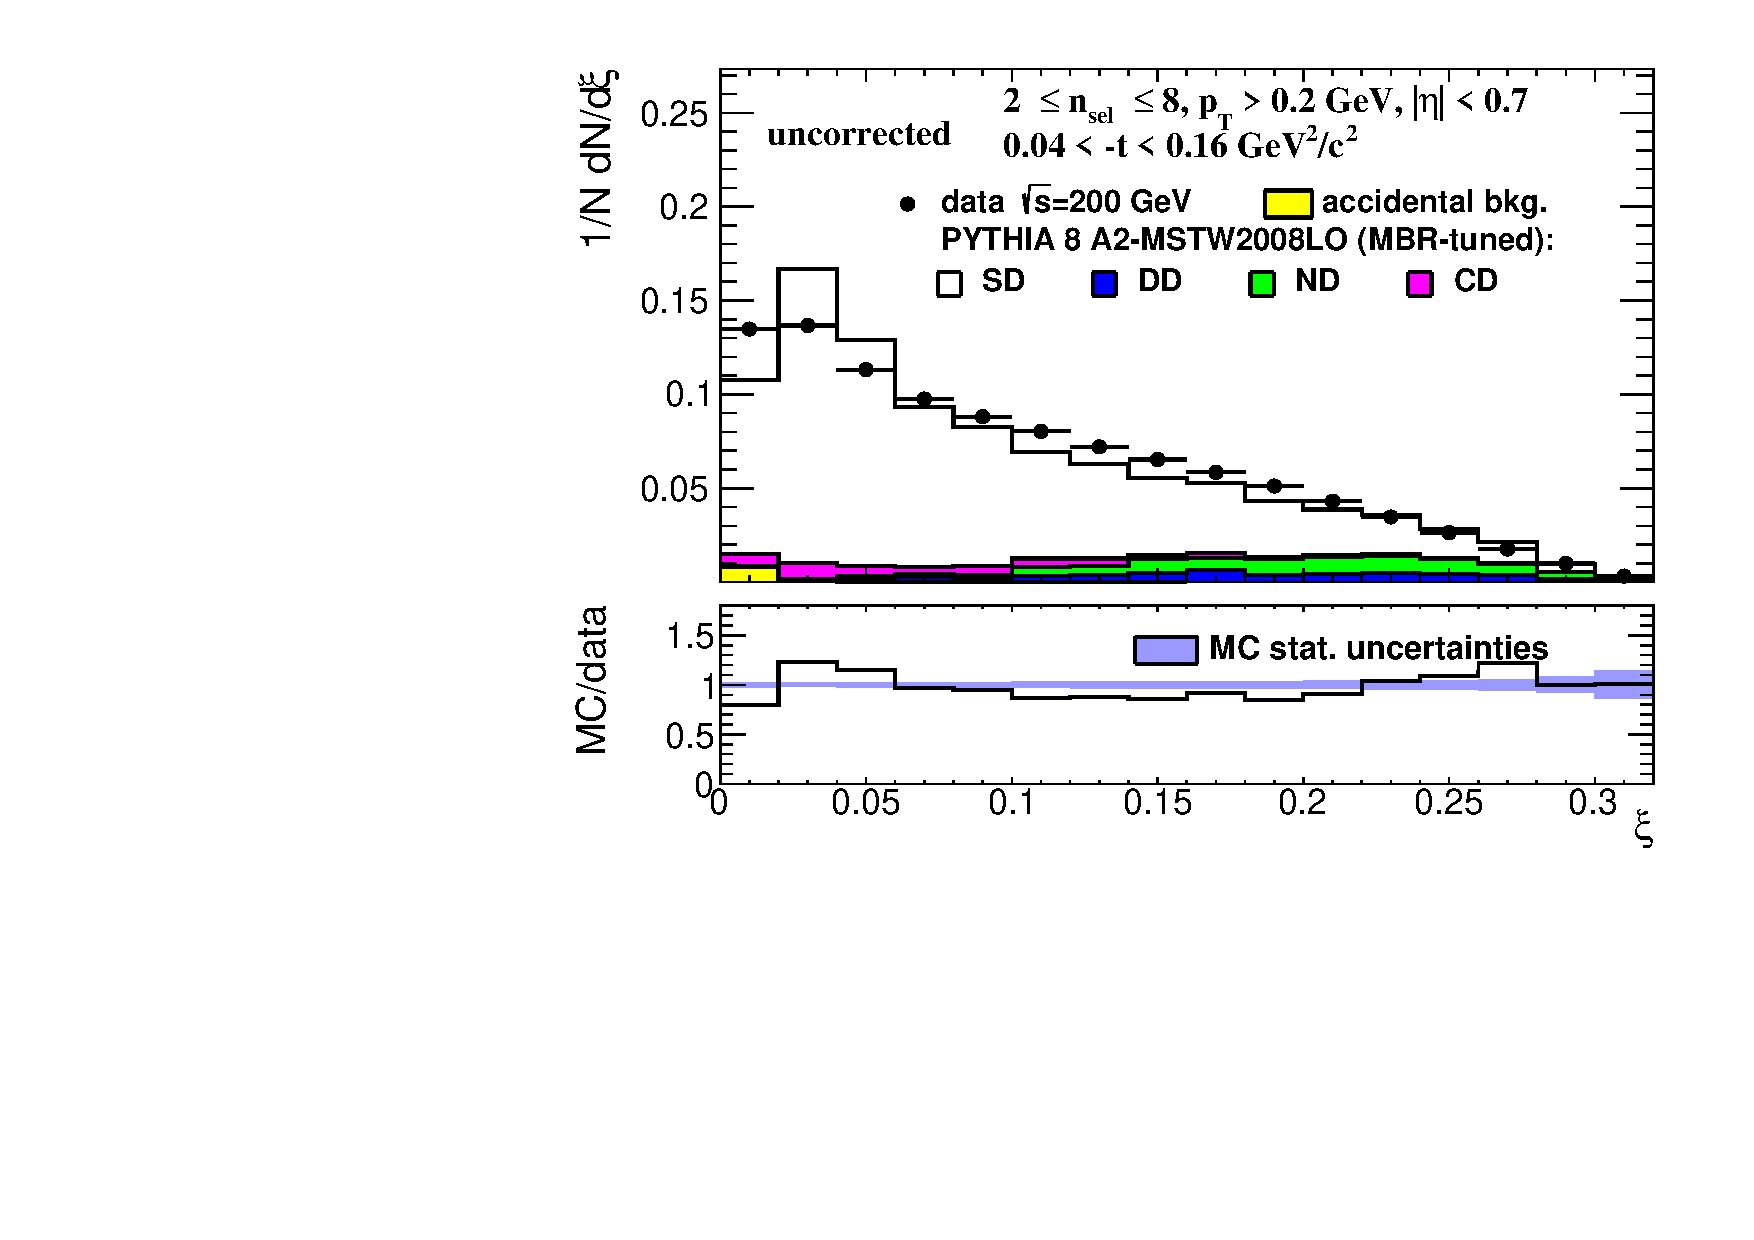
\includegraphics[width=.49\textwidth,page=1]{chapters/chrgSTAR/img/nonSD/SDT_pythia_xi0_option2_RP_starsim_xi.pdf}
\hfill
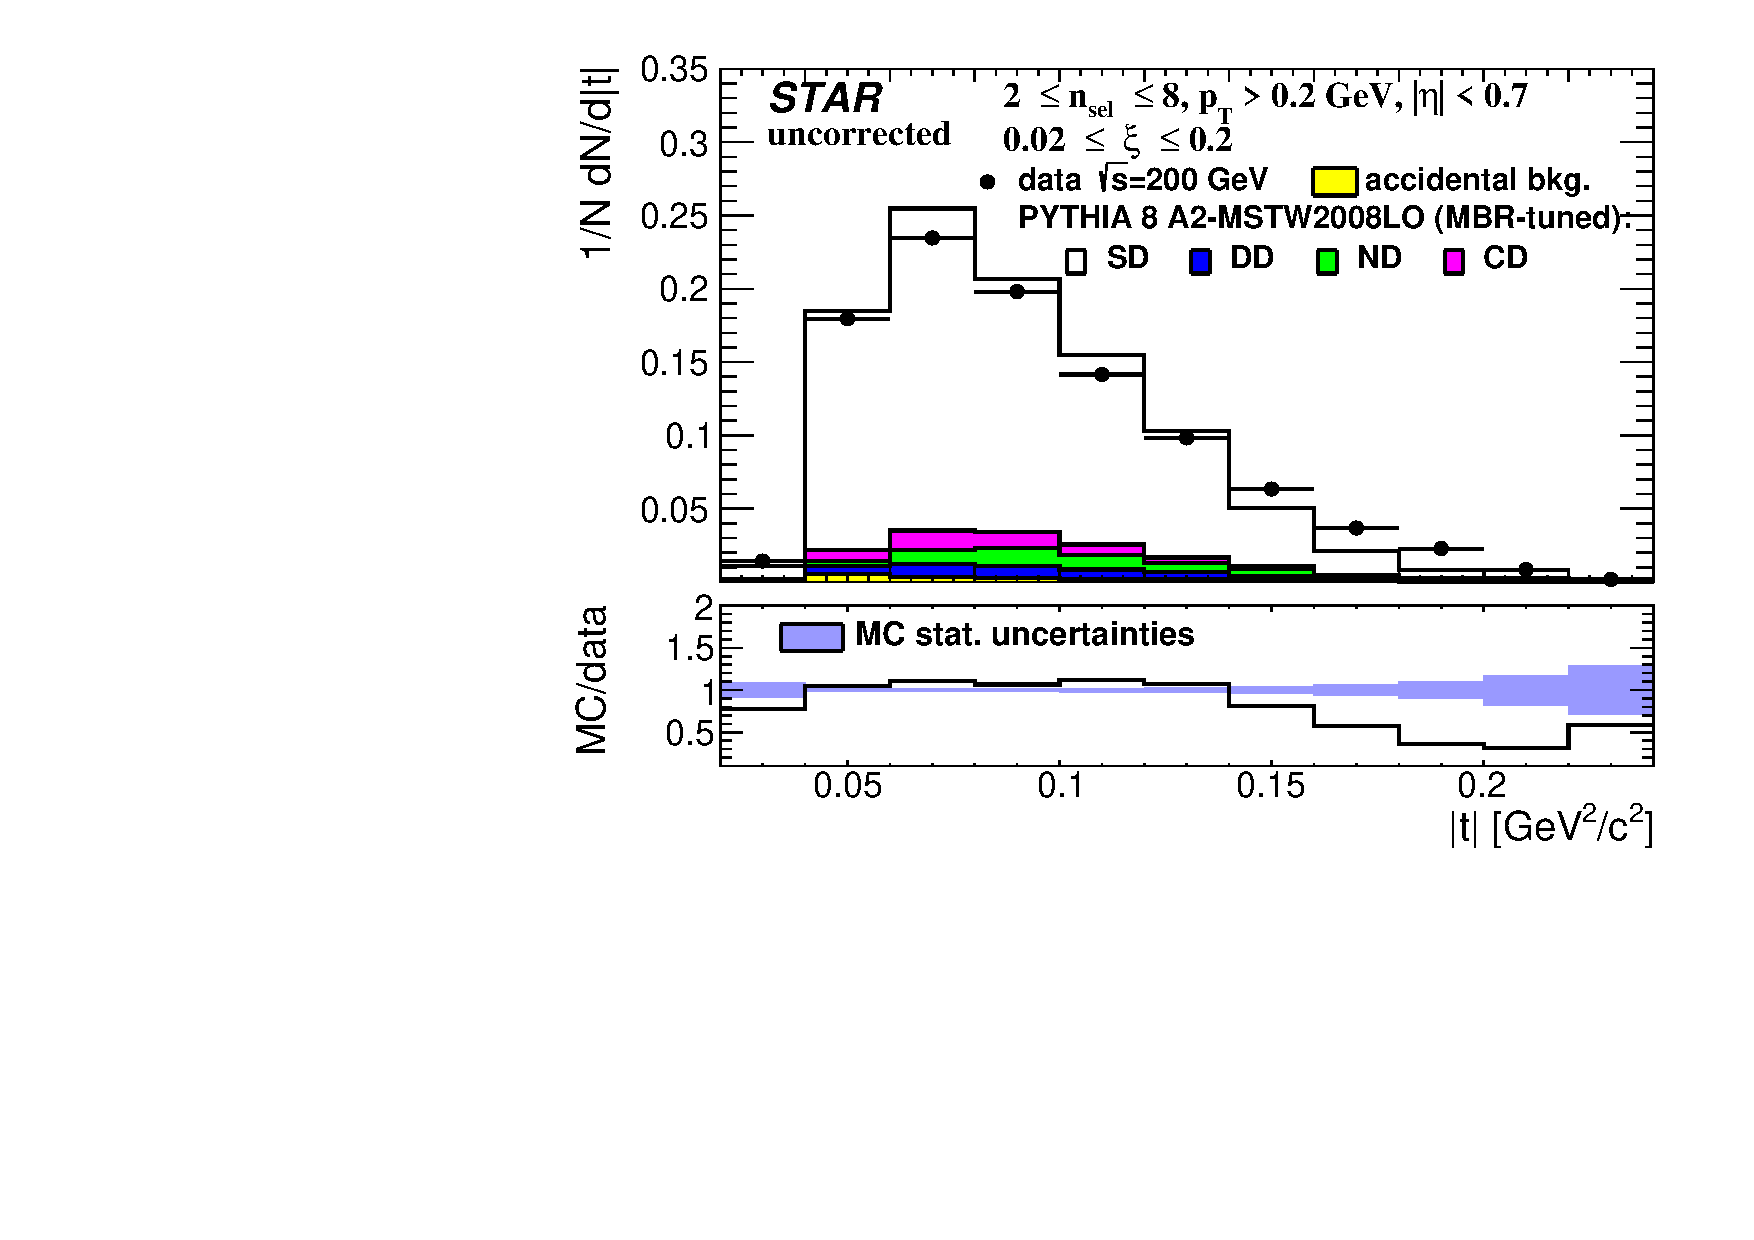
\includegraphics[width=.49\textwidth,page=1]{chapters/chrgSTAR/img/nonSD/SDT_pythia_xi0_option2_RP_starsim_t.pdf}
\newline
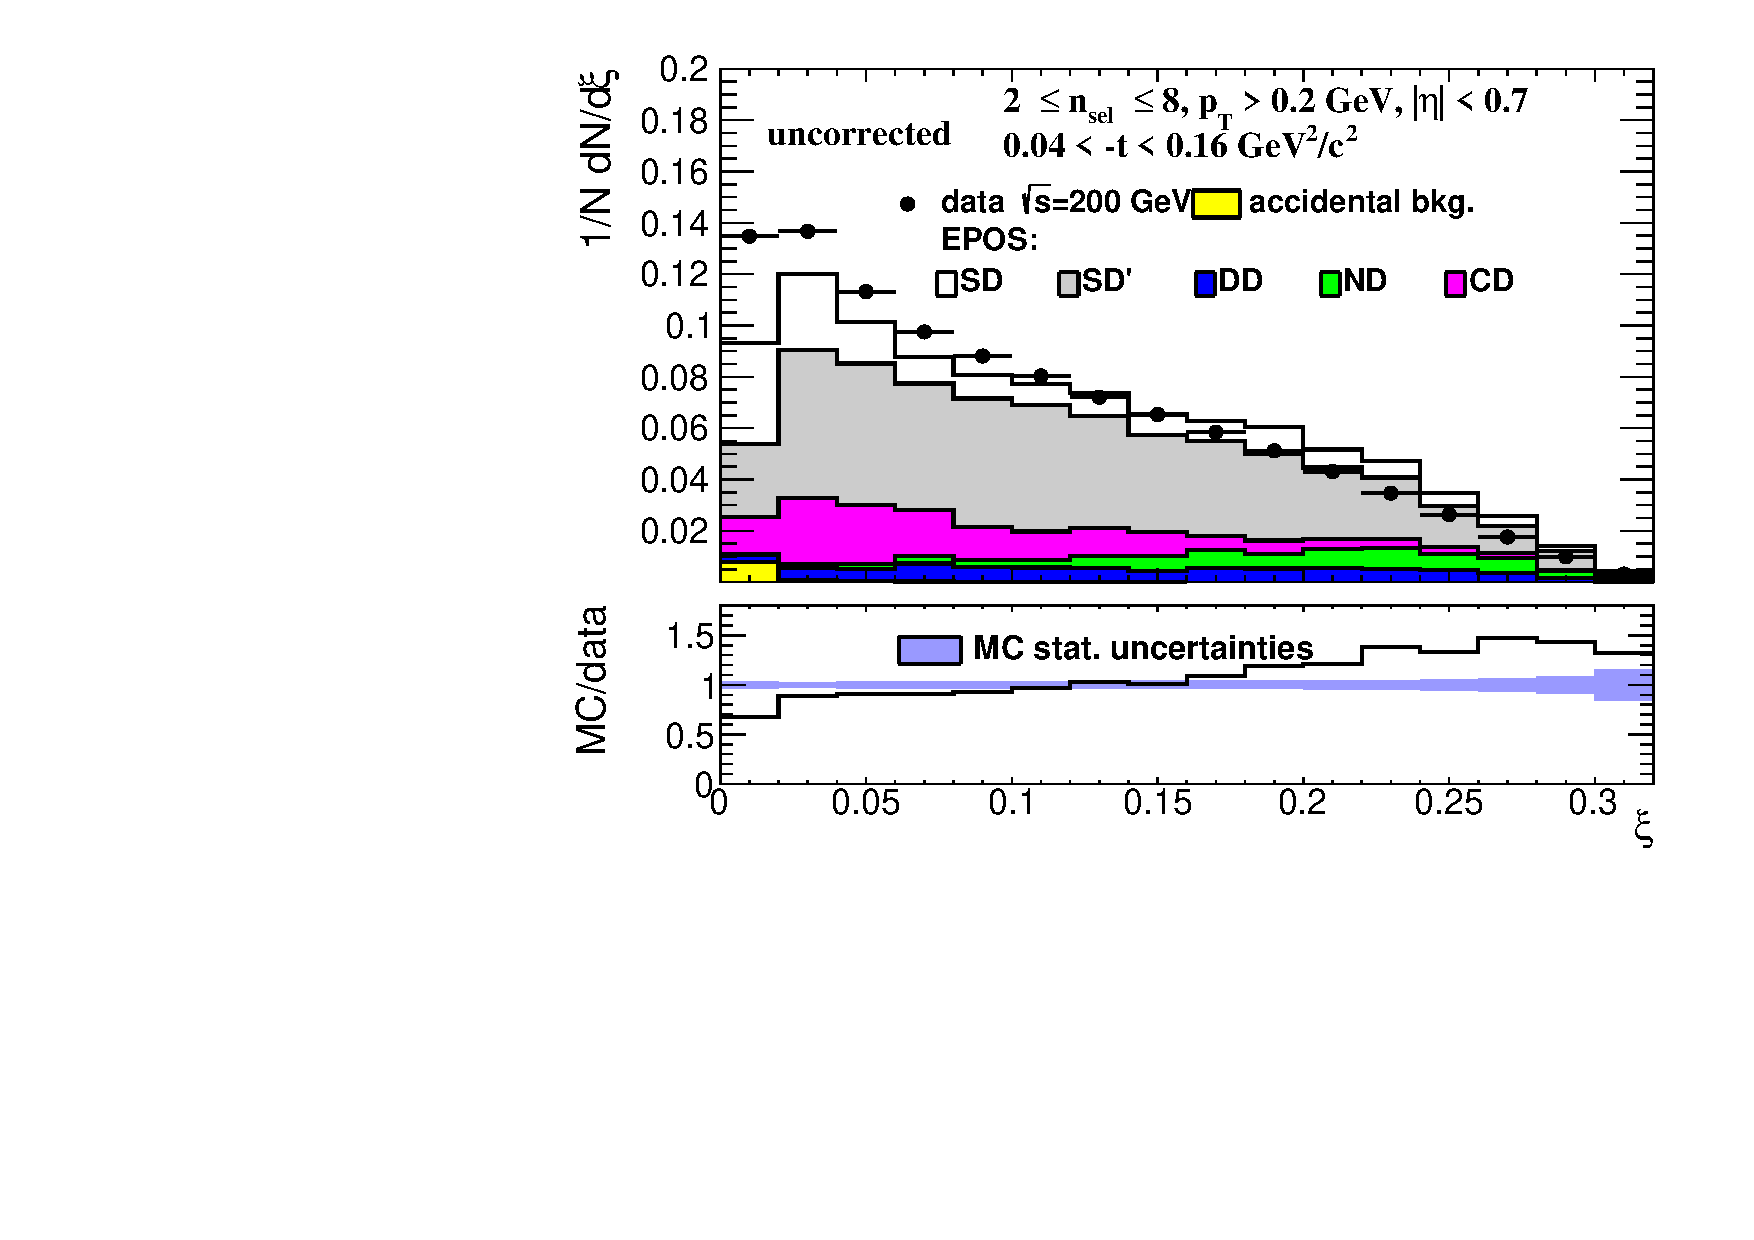
\includegraphics[width=.49\textwidth,page=1]{chapters/chrgSTAR/img/nonSD/SDT_epos_xi0_RP_starsim_xi.pdf}
\hfill
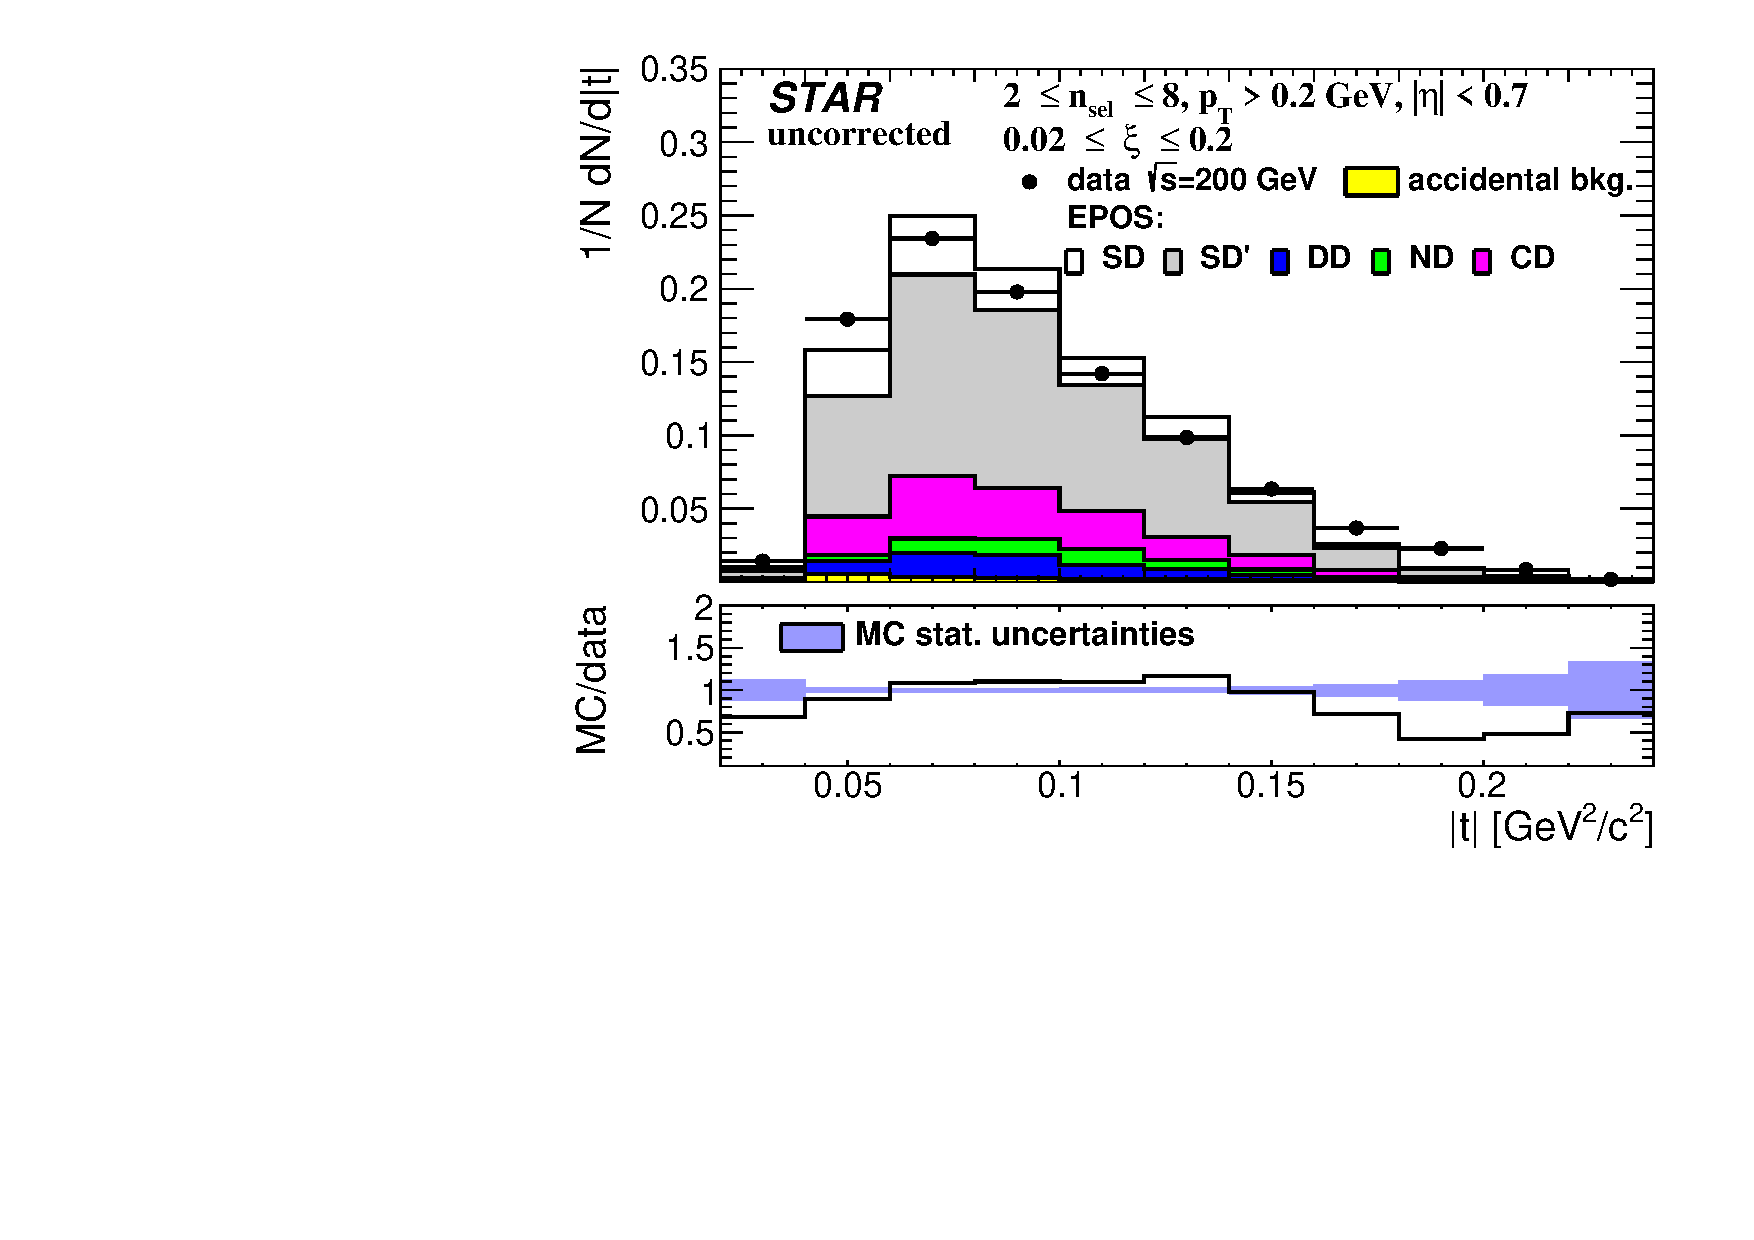
\includegraphics[width=.49\textwidth,page=1]{chapters/chrgSTAR/img/nonSD/SDT_epos_xi0_RP_starsim_t.pdf}
%
\caption{Uncorrected distributions of data compared to various MC models: (top) PYTHIA8 A2 (MBR), (middle) PYTHIA8 A2 (MBR-tuned) and (bottom) EPOS, as a function of (left column) $\xi$  and (right column) $|t|$.}
\label{fig:nonSDxit}
\end{figure}
\newpage

\begin{figure}[H]
\centering
\begin{subfigure}{.45\textwidth}
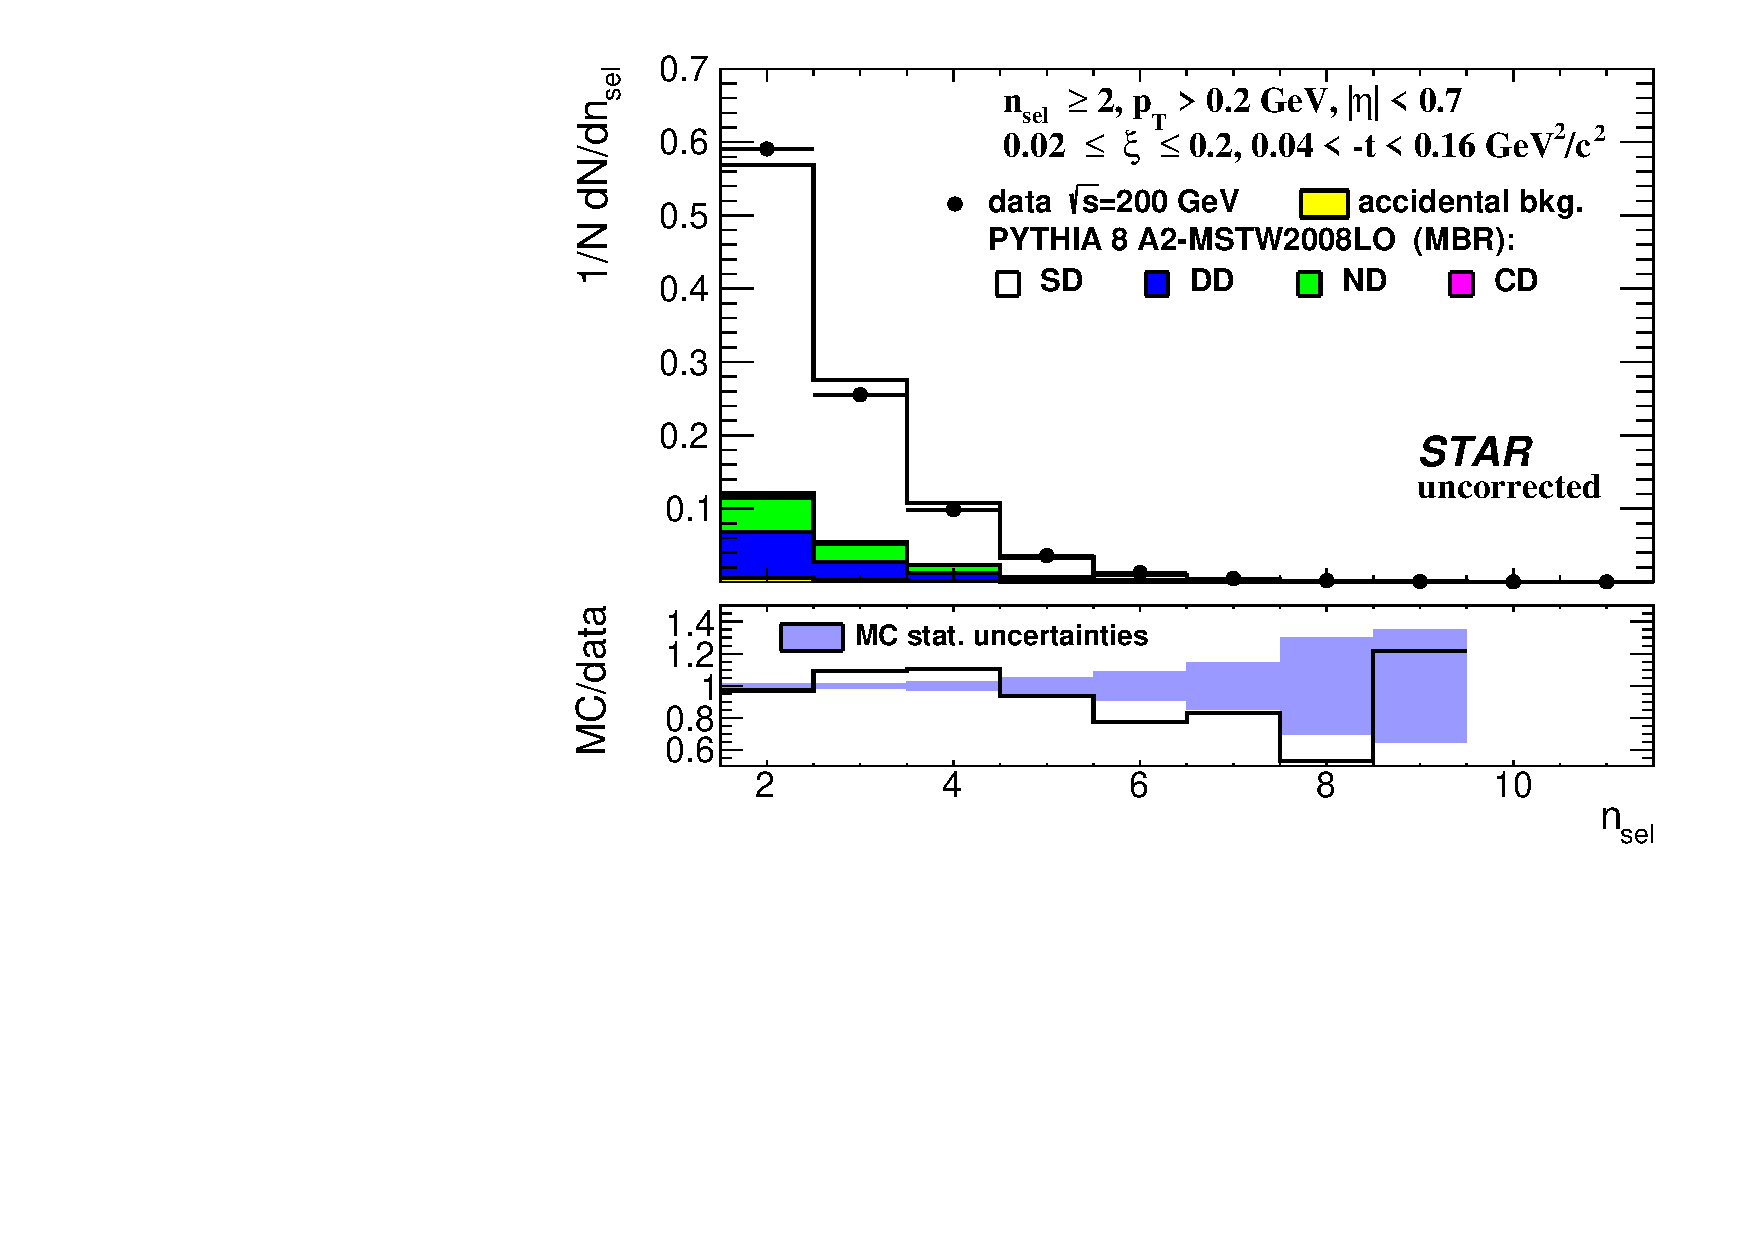
\includegraphics[width=\linewidth, page=1]{chapters/chrgSTAR/img/nonSD/chrg/SDT_pythia_xi0_RP_starsim_nsel.pdf}
\end{subfigure}
\begin{subfigure}{.45\textwidth}
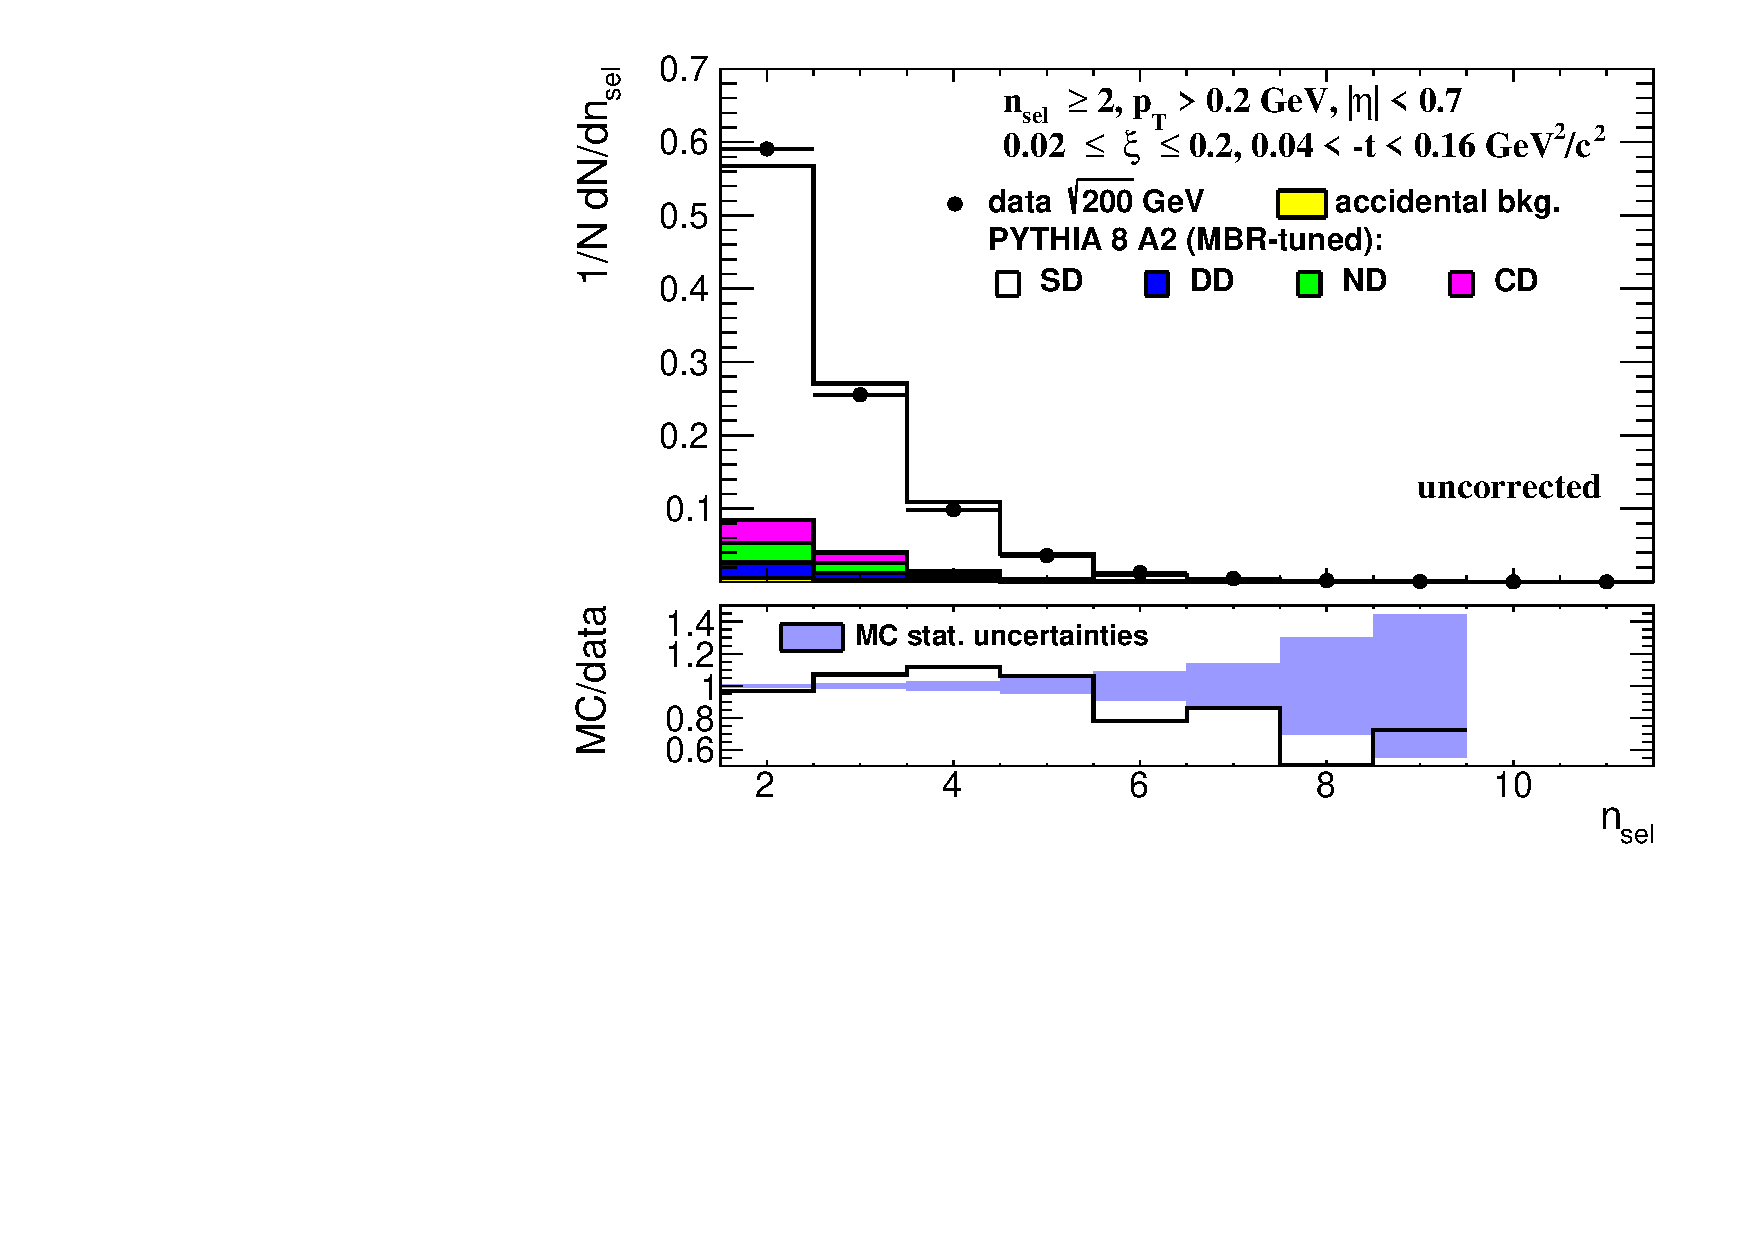
\includegraphics[width=\linewidth, page=1]{chapters/chrgSTAR/img/nonSD/chrg/SDT_pythia_xi0_option2_RP_starsim_nsel.pdf}
\end{subfigure}
\begin{subfigure}{.45\textwidth}
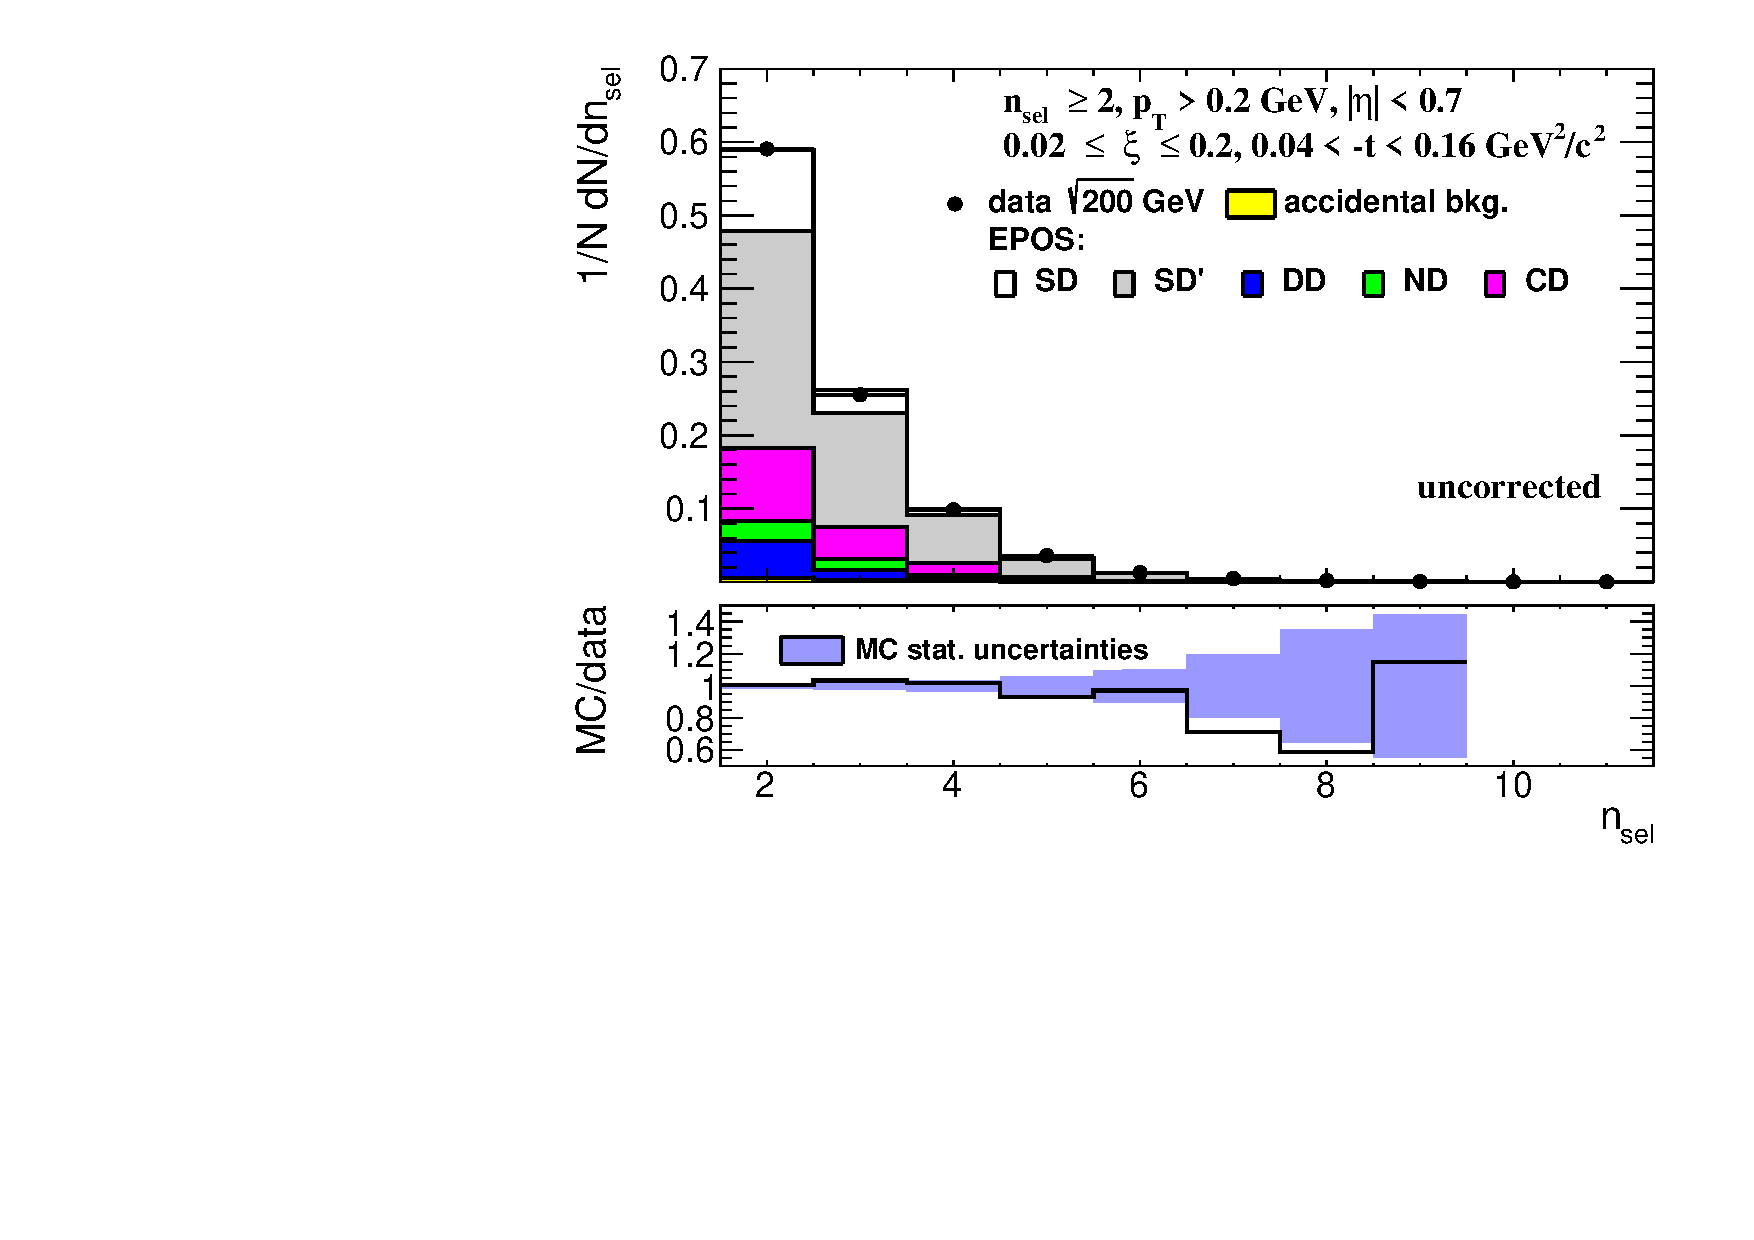
\includegraphics[width=\linewidth, page=1]{chapters/chrgSTAR/img/nonSD/chrg/SDT_epos_xi0_RP_starsim_nsel.pdf}
\end{subfigure}
\begin{minipage}{.45\textwidth}
\caption{Uncorrected distributions of data compared to various MC models: (top left) PYTHIA8 A2 (MBR), (top right) PYTHIA8 A2 (MBR-tuned) and (bottom) EPOS, as a function of $n_{\mathrm{sel}}$.}
\label{fig:nonSDnsel}
\end{minipage}

\end{figure}
\begin{figure}[H]
%	\vspace{-0.5cm}
\centering
\begin{subfigure}{.45\textwidth}
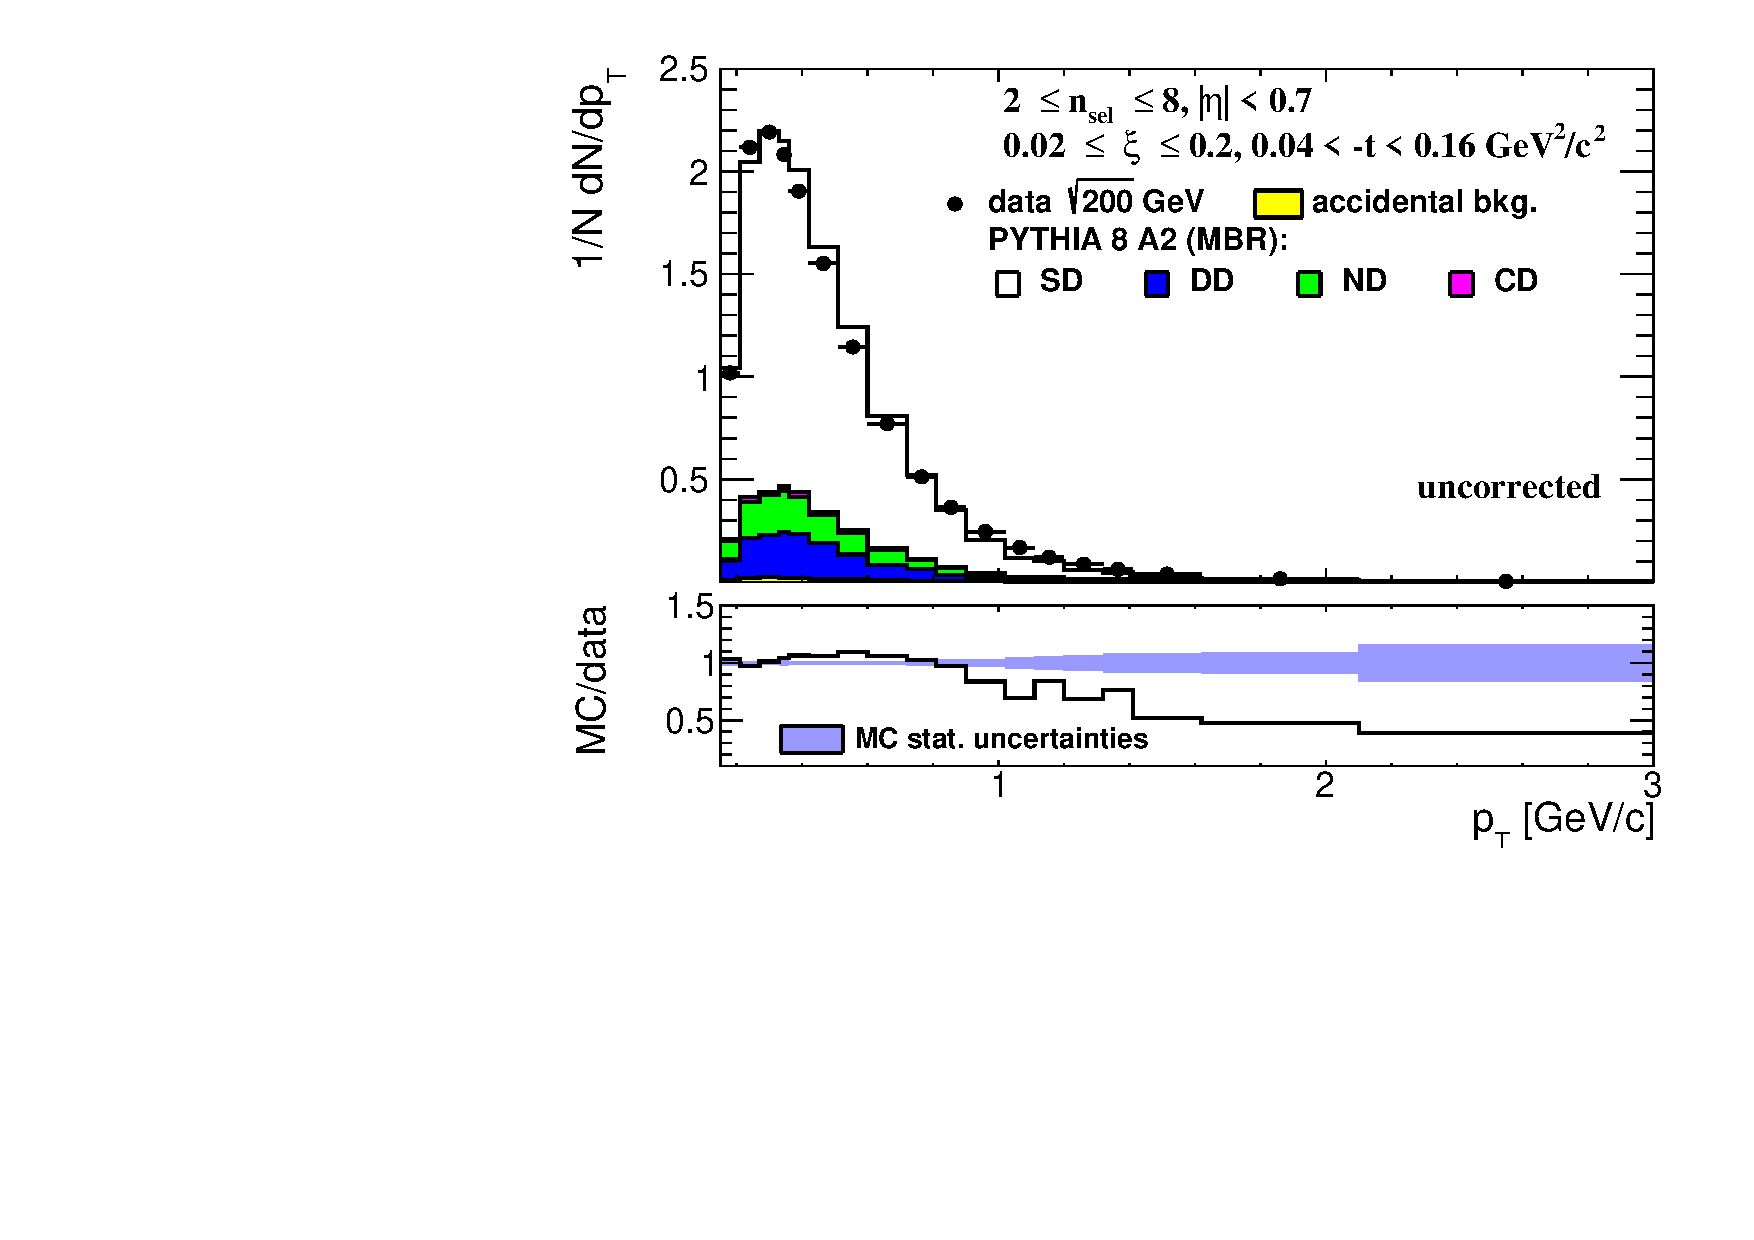
\includegraphics[width=\linewidth, page=1]{chapters/chrgSTAR/img/nonSD/chrg/SDT_pythia_xi0_RP_starsim_pt.pdf}
\end{subfigure}
\begin{subfigure}{.45\textwidth}
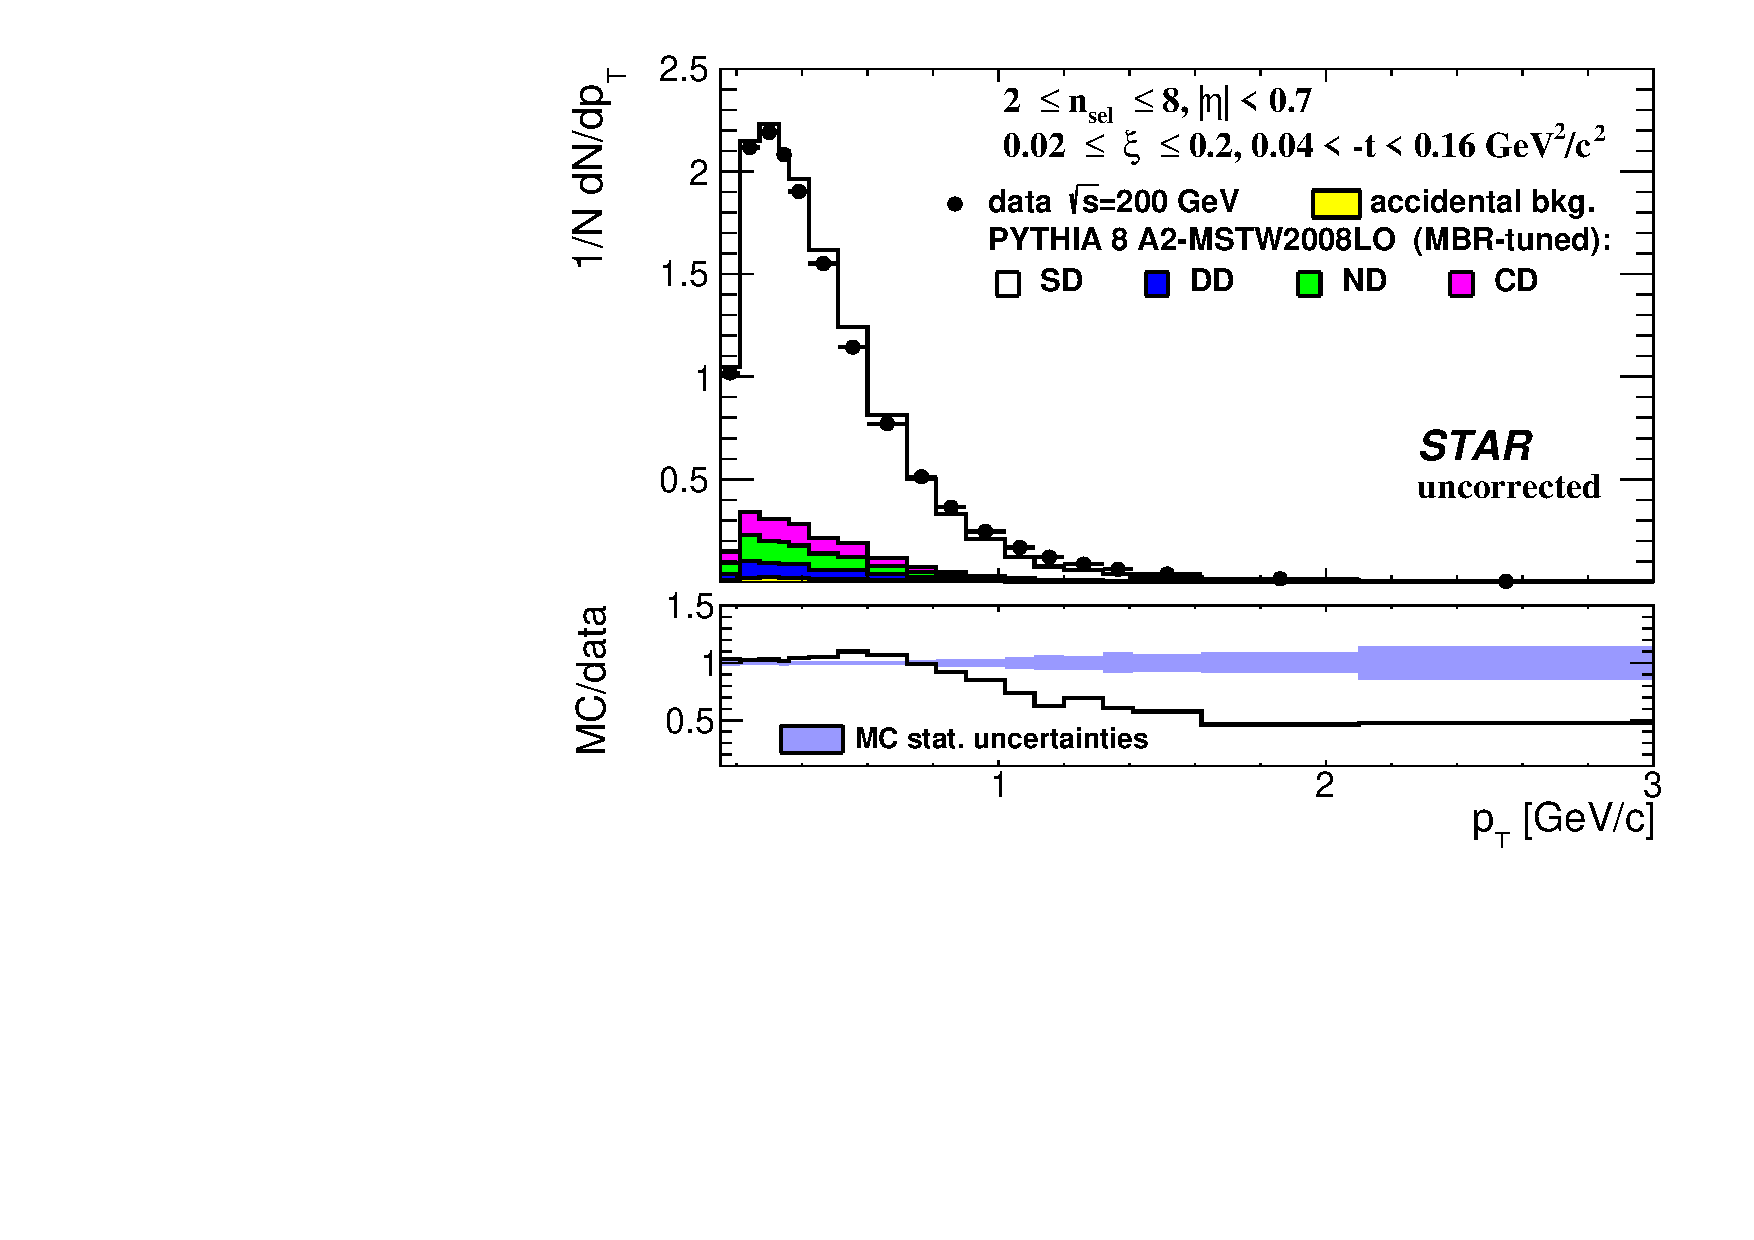
\includegraphics[width=\linewidth, page=1]{chapters/chrgSTAR/img/nonSD/chrg/SDT_pythia_xi0_option2_RP_starsim_pt.pdf}
\end{subfigure}
\begin{subfigure}{.45\textwidth}
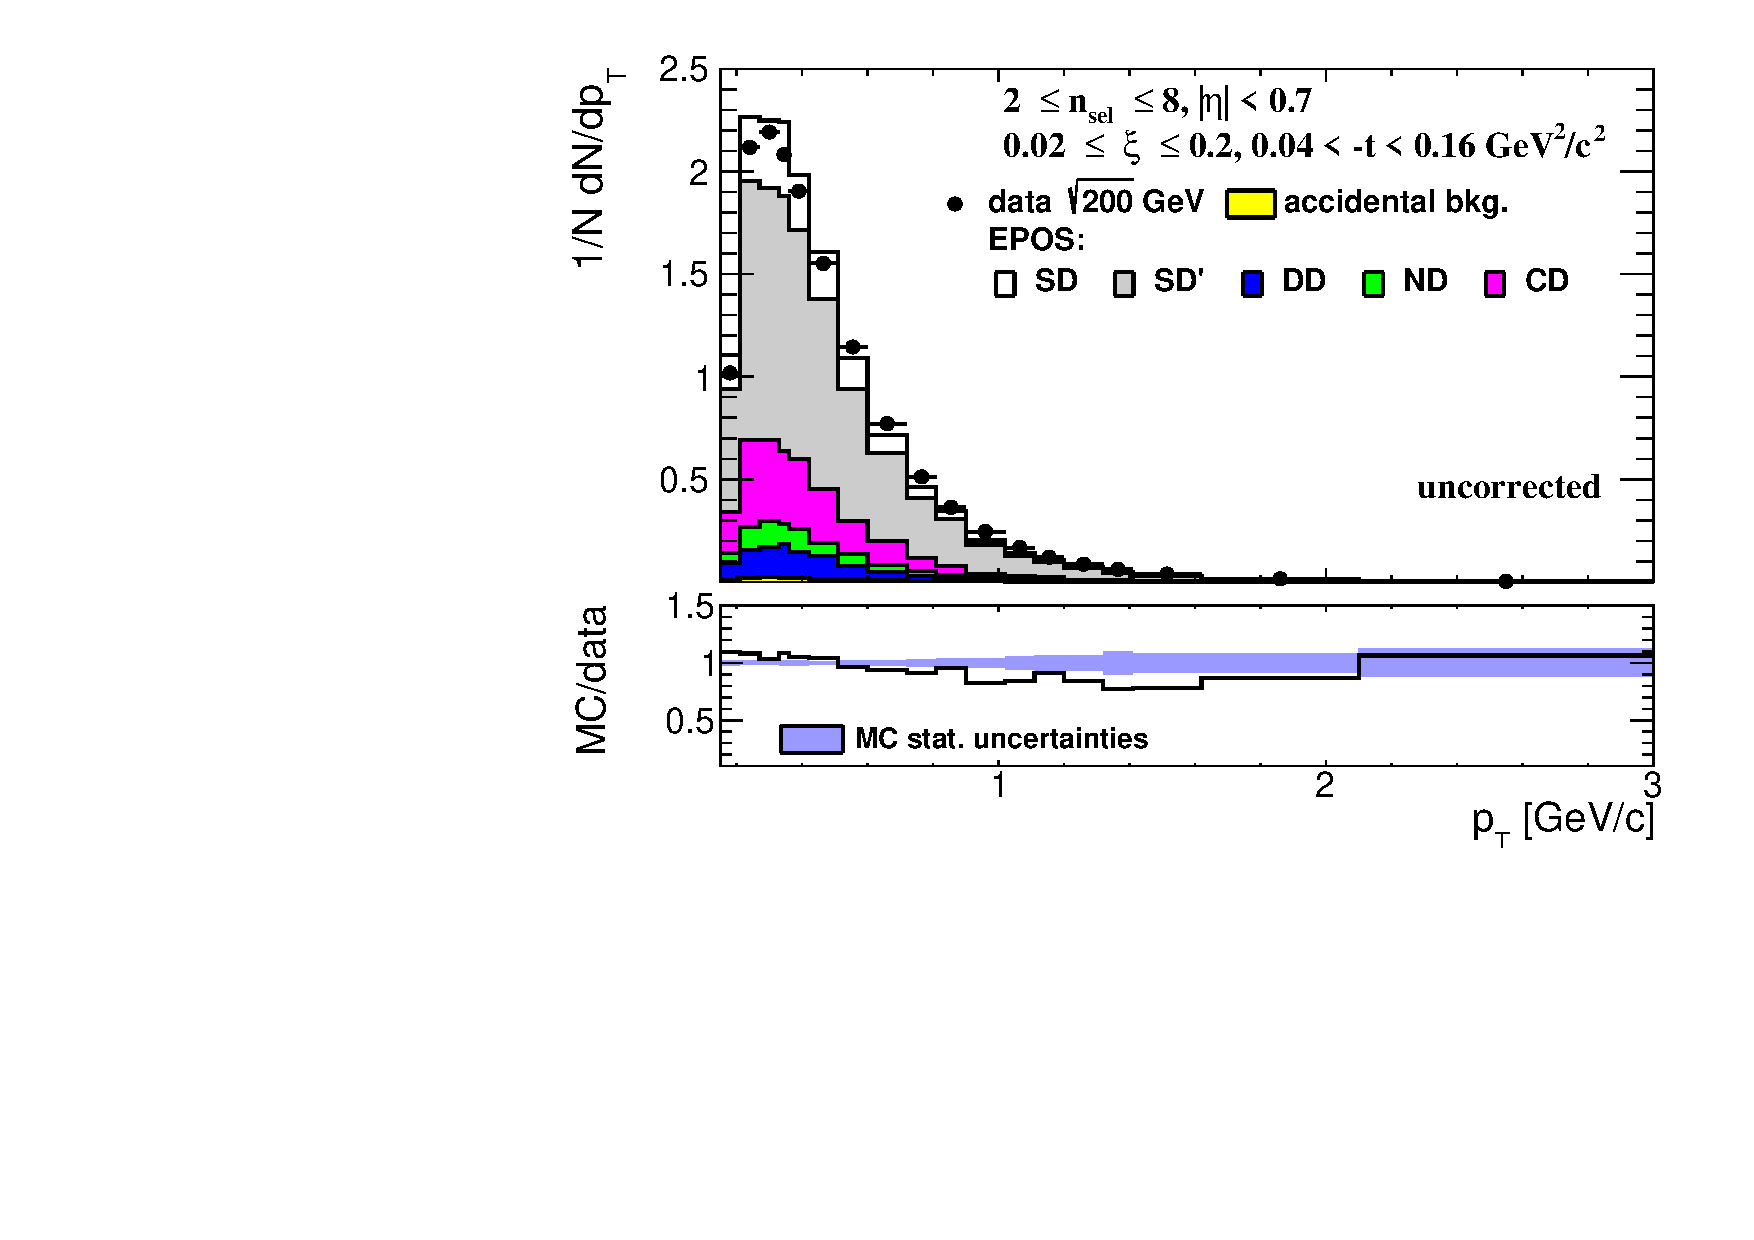
\includegraphics[width=\linewidth, page=1]{chapters/chrgSTAR/img/nonSD/chrg/SDT_epos_xi0_RP_starsim_pt.pdf}
\end{subfigure}
\begin{minipage}{.45\textwidth}
\caption{Uncorrected distributions of data compared to various MC models: (top left) PYTHIA8 A2 (MBR), (top right) PYTHIA8 A2 (MBR-tuned) and (bottom) EPOS, as a function of $p_{\mathrm{T}}$.}
\label{fig:nonSDpt}
\end{minipage}

\end{figure}
\newpage
\begin{figure}[H]
%	\vspace{-0.5cm}
\centering
\begin{subfigure}{.45\textwidth}
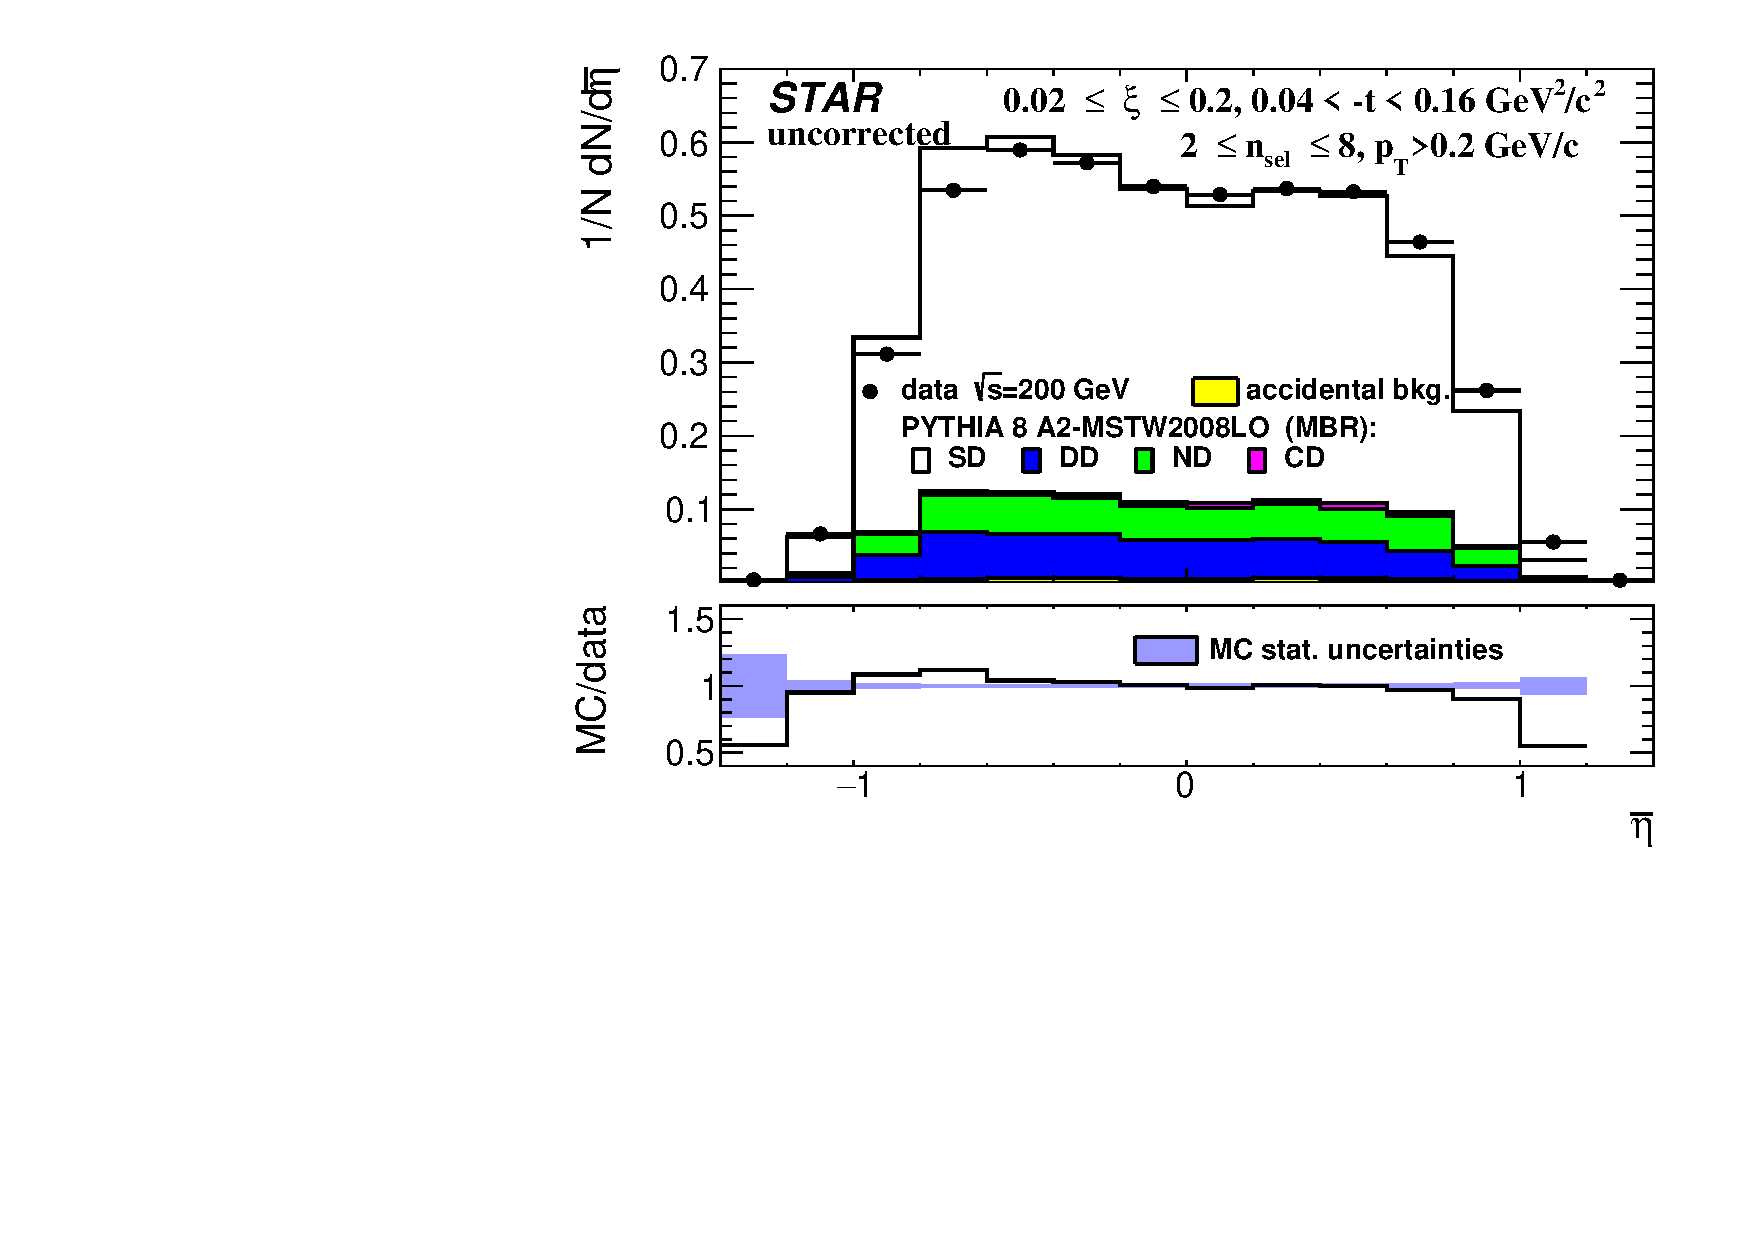
\includegraphics[width=\linewidth, page=1]{chapters/chrgSTAR/img/nonSD/chrg/SDT_pythia_xi0_RP_starsim_eta.pdf}
\end{subfigure}
\begin{subfigure}{.45\textwidth}
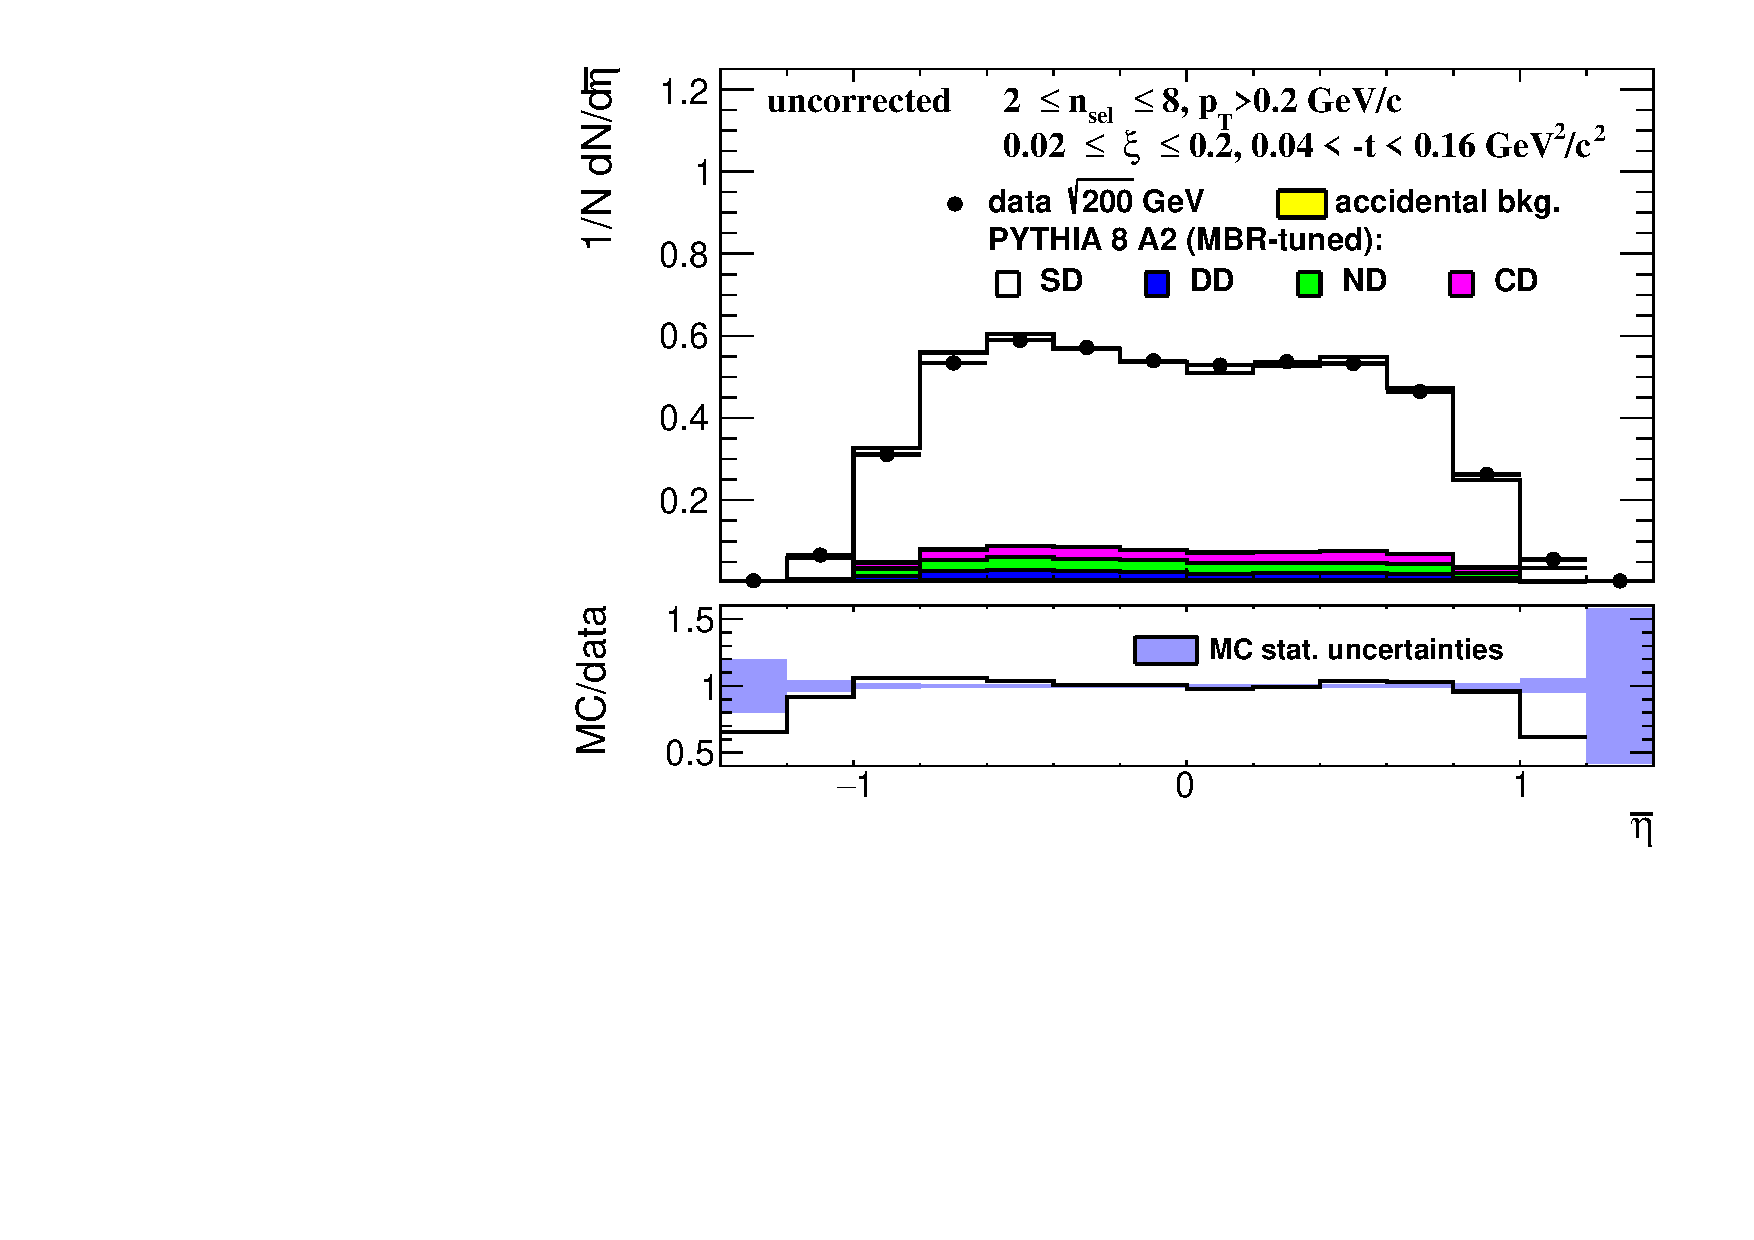
\includegraphics[width=\linewidth, page=1]{chapters/chrgSTAR/img/nonSD/chrg/SDT_pythia_xi0_option2_RP_starsim_eta.pdf}
\end{subfigure}
\begin{subfigure}{.45\textwidth}
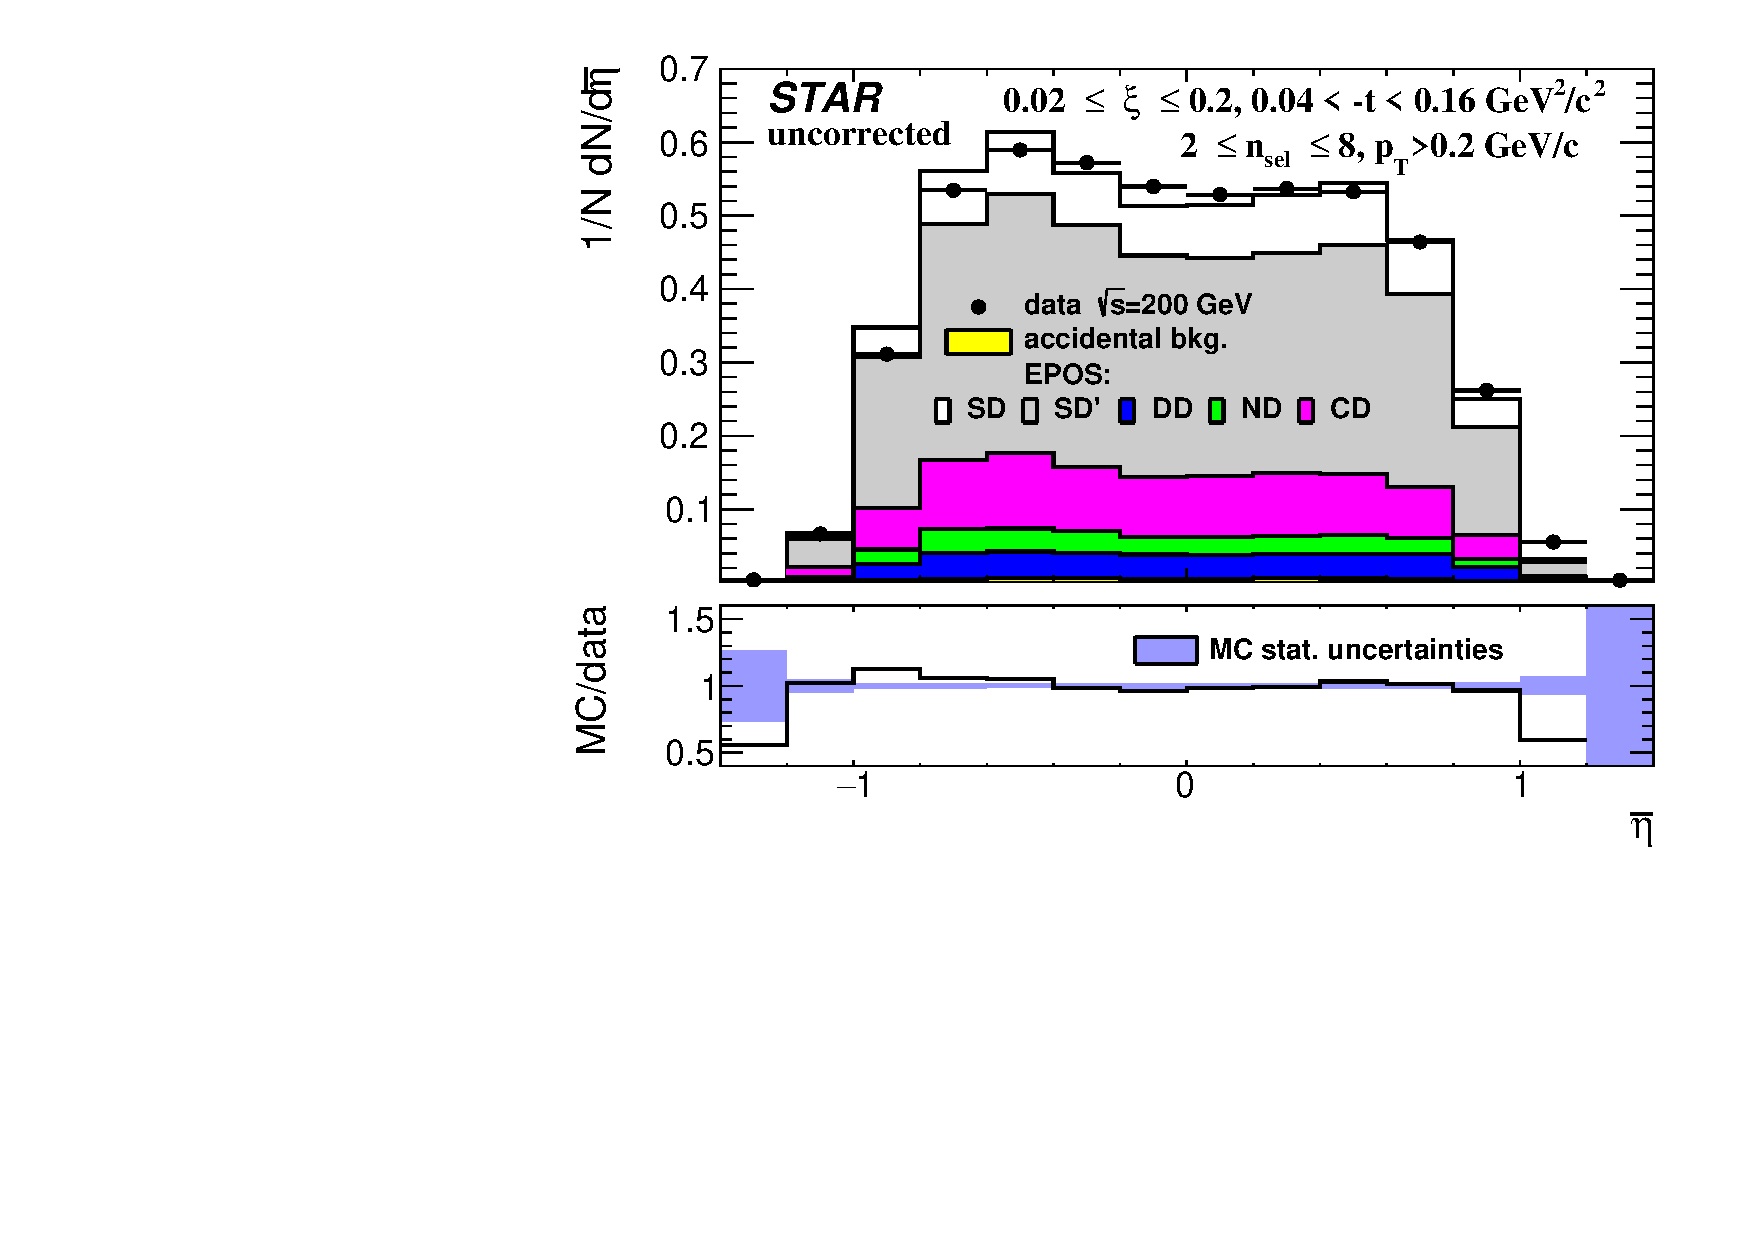
\includegraphics[width=\linewidth, page=1]{chapters/chrgSTAR/img/nonSD/chrg/SDT_epos_xi0_RP_starsim_eta.pdf}
\end{subfigure}
\begin{minipage}{.45\textwidth}
\caption{Uncorrected distributions of data compared to various MC models: (top left) PYTHIA8 A2 (MBR), (top right) PYTHIA8 A2 (MBR-tuned) and (bottom) EPOS, as a function of $\bar{\eta}$. }
\label{fig:nonSDera}
\end{minipage}

\end{figure}
\end{comment}
Events, in which  forward-scattered proton and reconstructed TOF
vertex are the result of the same $pp$ interaction, may originate from \ac{ND}, \ac{DD}, \ac{SD}, and \ac{CD} processes.  It is preferred to estimate the~background contribution from data, using dedicated control regions.
Since such regions were not found, the~relative contributions from the~above processes were  estimated from MC models and are therefore model dependent. Tracks reconstructed in \ac{RP}s  %which are modeled in the~\ac{MC} simulations are only coming from:
may also be:
\begin{itemize}
	\item forward-scattered protons produced in the \ac{SD}, \ac{CD} or \ac{DD} diffractive systems or from \ac{ND} events,
	\item secondary particles from showering initiated 
	by interaction of forward-scattered protons with beam-line elements. This contribution is negligible.
\end{itemize}


Figure~\ref{fig:nonSDxit} shows the uncorrected $\xi$ and $t$ distributions in data compared to various \ac{MC} models: PYTHIA~8 A2 (MBR), PYTHIA~8 A2 (MBR-tuned), PYTHIA~8 4C (SaS) and EPOS. The \ac{MC} distributions are split into \ac{SD}, \ac{ND}, \ac{DD} and \ac{CD} components. For EPOS, SD$^\prime$ is separated from the ND events. Additionally, the accidental background is also shown. PYTHIA~8 A2 (MBR) predictions, shown in Fig.~\ref{fig:nonSDxit} (a-b), do not agree with the data, especially  there is small number of events in the~region of large values of $\xi$. 
This effect may be due to the~scaling factors, which are introduced in PYTHIA~8 to artificially suppress diffractive cross sections in the~high mass region, or due to too large Pomeron intercept ($\epsilon=0.104$).
 Therefore,
additional two samples of PYTHIA~8 were generated: without this artificial suppression  (\mbox{MBR-tuned}) and with  $\epsilon=0$ (\mbox{SaS}). Their predictions, shown in Fig.~\ref{fig:nonSDxit} (c-f), agree much better with the~data than PYTHIA~8 A2 (MBR) and result also in a~suppression of non-SD events. Amongst PYTHIA~8 models, PYTHIA~8 A2 (MBR-tuned) shows the~best agreement  with the~data.
EPOS predictions,  shown in Fig.~\ref{fig:nonSDxit} (g-h), describes data better than PYTHIA~8 but shows a dominant contribution of SD$^\prime$ events. The~CD contribution in EPOS is several times greater than in PYTHIA~8 (MBR), but it was never tuned to describe any data, as opposed to PYTHIA~8 (MBR) in which the~\ac{CD} cross sections are constrained by CDF measurements~\cite{Acosta:2003xi}. 
The~\ac{CD} component in the~\ac{SaS} model is based on simple scaling assumption, therefore, it is not usually used by the~experimental communities. All MCs predict significant \ac{DD} and \ac{ND} background at large $\xi$, thereby  the analysis was limited to $\xi < 0.2$. 


\Cref{fig:nonSDnsel,fig:nonSDpt,fig:nonSDera} show the uncorrected distributions of variables used in the later analysis: $n_{\mathrm{sel}}$, $p_{\mathrm T}$ an $\bar{\eta}$. The  contributions from non-SD (except  EPOS SD$^\prime$) interactions differ a bit between each other, i.e. EPOS predicts significantly larger CD contribution, whereas DD and ND are suppressed in PYTHIA~8 A2 (MBR-tuned) and PYTHIA~8 4C (SaS).  PYTHIA~8~A2~(MBR) is used as the default model  of non-SD contribution subtracted from the data with systematic uncertainty $\pm50\%$, which covers all differences between the~models except EPOS SD$^\prime$.  In this analysis EPOS SD$^\prime$ is   considered as an~alternative to PYTHIA~8 SD model of events with forward-scattered proton in the final state,  where one of the proton remnants hadronizes back to a~single proton (non-diffractive process), while in  PYTHIA~8 the~initial proton stays intact (diffractive process). As a~consequence, results  are compared  with the~sum of SD and SD$^\prime$ processes for EPOS model.  
%\end{comment}
%\thispagestyle{empty}

%\newpage
\begin{figure}[H]
	%\vspace{-1.cm}
	\thisfloatpagestyle{fancy}
	\centering
	\begin{overpic}[width=0.47\textwidth,tics=4,page=1]{chapters/chrgSTAR/img/nonSD/SDT_pythia_xi0_RP_starsim_xi.pdf}
		\put (88,40) {\Large{a}}
	\end{overpic}
	\vspace{-0.2cm}
	\begin{overpic}[width=0.47\textwidth,tics=4,page=1]{chapters/chrgSTAR/img/nonSD/SDT_pythia_xi0_RP_starsim_t.pdf}
		\put (85,35) {\Large{b}}
	\end{overpic}
	\begin{overpic}[width=0.47\textwidth,tics=4,page=1]{chapters/chrgSTAR/img/nonSD/SDT_pythia_xi0_option2_RP_starsim_xi.pdf}
		\put (85,35) {\Large{c}}
	\end{overpic}
	\vspace{-0.2cm}
	\begin{overpic}[width=0.47\textwidth,tics=4,page=1]{chapters/chrgSTAR/img/nonSD/SDT_pythia_xi0_option2_RP_starsim_t.pdf}
		\put (85,35) {\Large{d}}
	\end{overpic}
	\begin{overpic}[width=0.47\textwidth,tics=4,page=1]{chapters/chrgSTAR/img/nonSD/SDT_pythia_xi0_sas_RP_starsim_xi.pdf}
		\put (85,35) {\Large{e}}
	\end{overpic}
	\vspace{-0.2cm}
	\begin{overpic}[width=0.47\textwidth,tics=4,page=1]{chapters/chrgSTAR/img/nonSD/SDT_pythia_xi0_sas_RP_starsim_t.pdf}
		\put (85,35) {\Large{f}}
	\end{overpic}
	\begin{overpic}[width=0.47\textwidth,tics=4,page=1]{chapters/chrgSTAR/img/nonSD/SDT_epos_xi0_RP_starsim_xi.pdf}
		\put (85,35) {\Large{g}}
	\end{overpic}
	\vspace{-0.2cm}
	\begin{overpic}[width=0.47\textwidth,tics=4,page=1]{chapters/chrgSTAR/img/nonSD/SDT_epos_xi0_RP_starsim_t.pdf}
		\put (85,35) {\Large{h}}
	\end{overpic}
	\vspace{-0.2cm}
	%
	\caption{Uncorrected distributions of data compared to various MC models: (a-b) PYTHIA~8 A2 (MBR), (c-d) PYTHIA~8 A2 (MBR-tuned), (e-f) PYTHIA~8 4C (SaS) and (g-h) EPOS, as a~function of (left column) $\xi$  and (right column) $|t|$. The~ratio of MC predictions and data is shown in the~bottom panels.}
	\label{fig:nonSDxit}
	%\vspace{-0.5cm}
\end{figure}

\begin{figure}[t!]
	\vspace{-1.5cm}
	\thisfloatpagestyle{fancy}
	\centering
	\begin{subfigure}{.49\textwidth}
		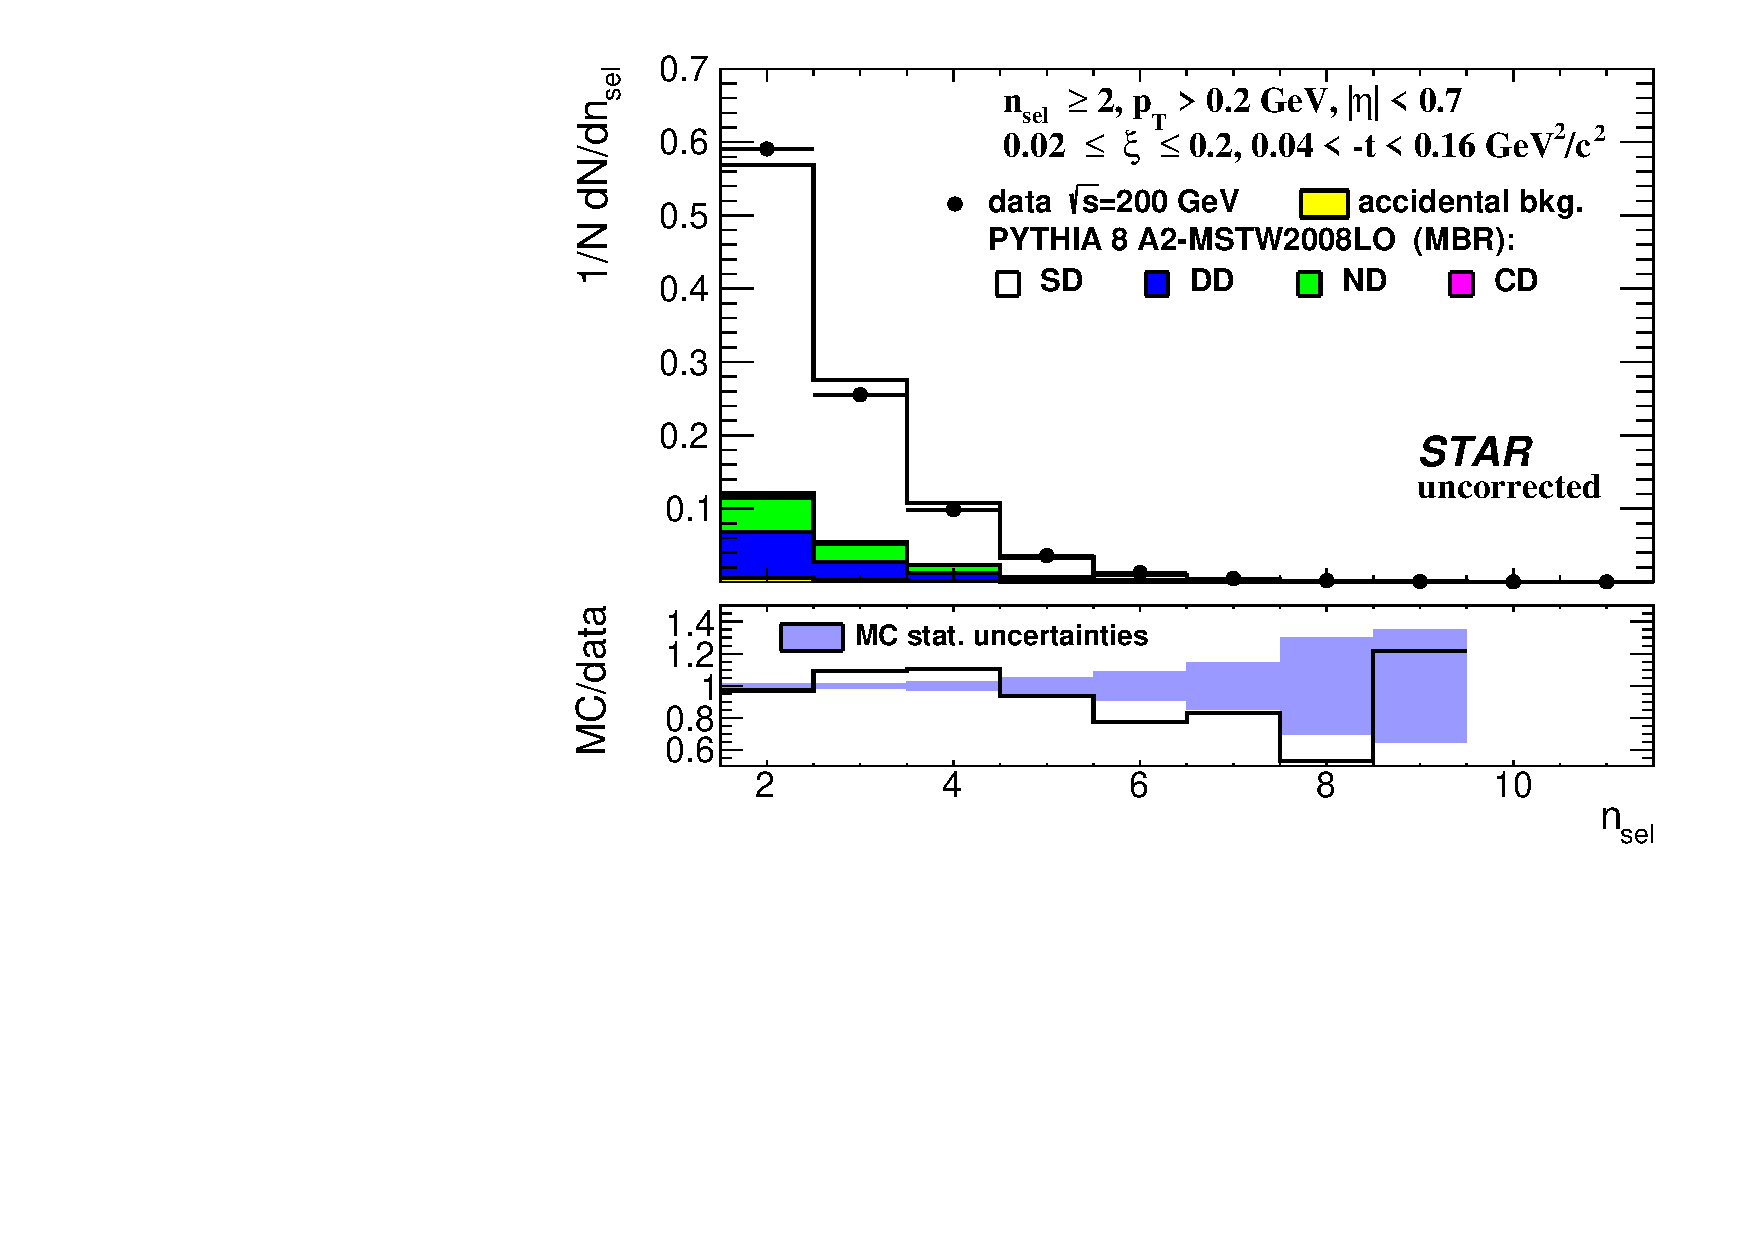
\includegraphics[width=\linewidth, page=1]{chapters/chrgSTAR/img/nonSD/chrg/SDT_pythia_xi0_RP_starsim_nsel.pdf}
	\end{subfigure}
	\begin{subfigure}{.49\textwidth}
		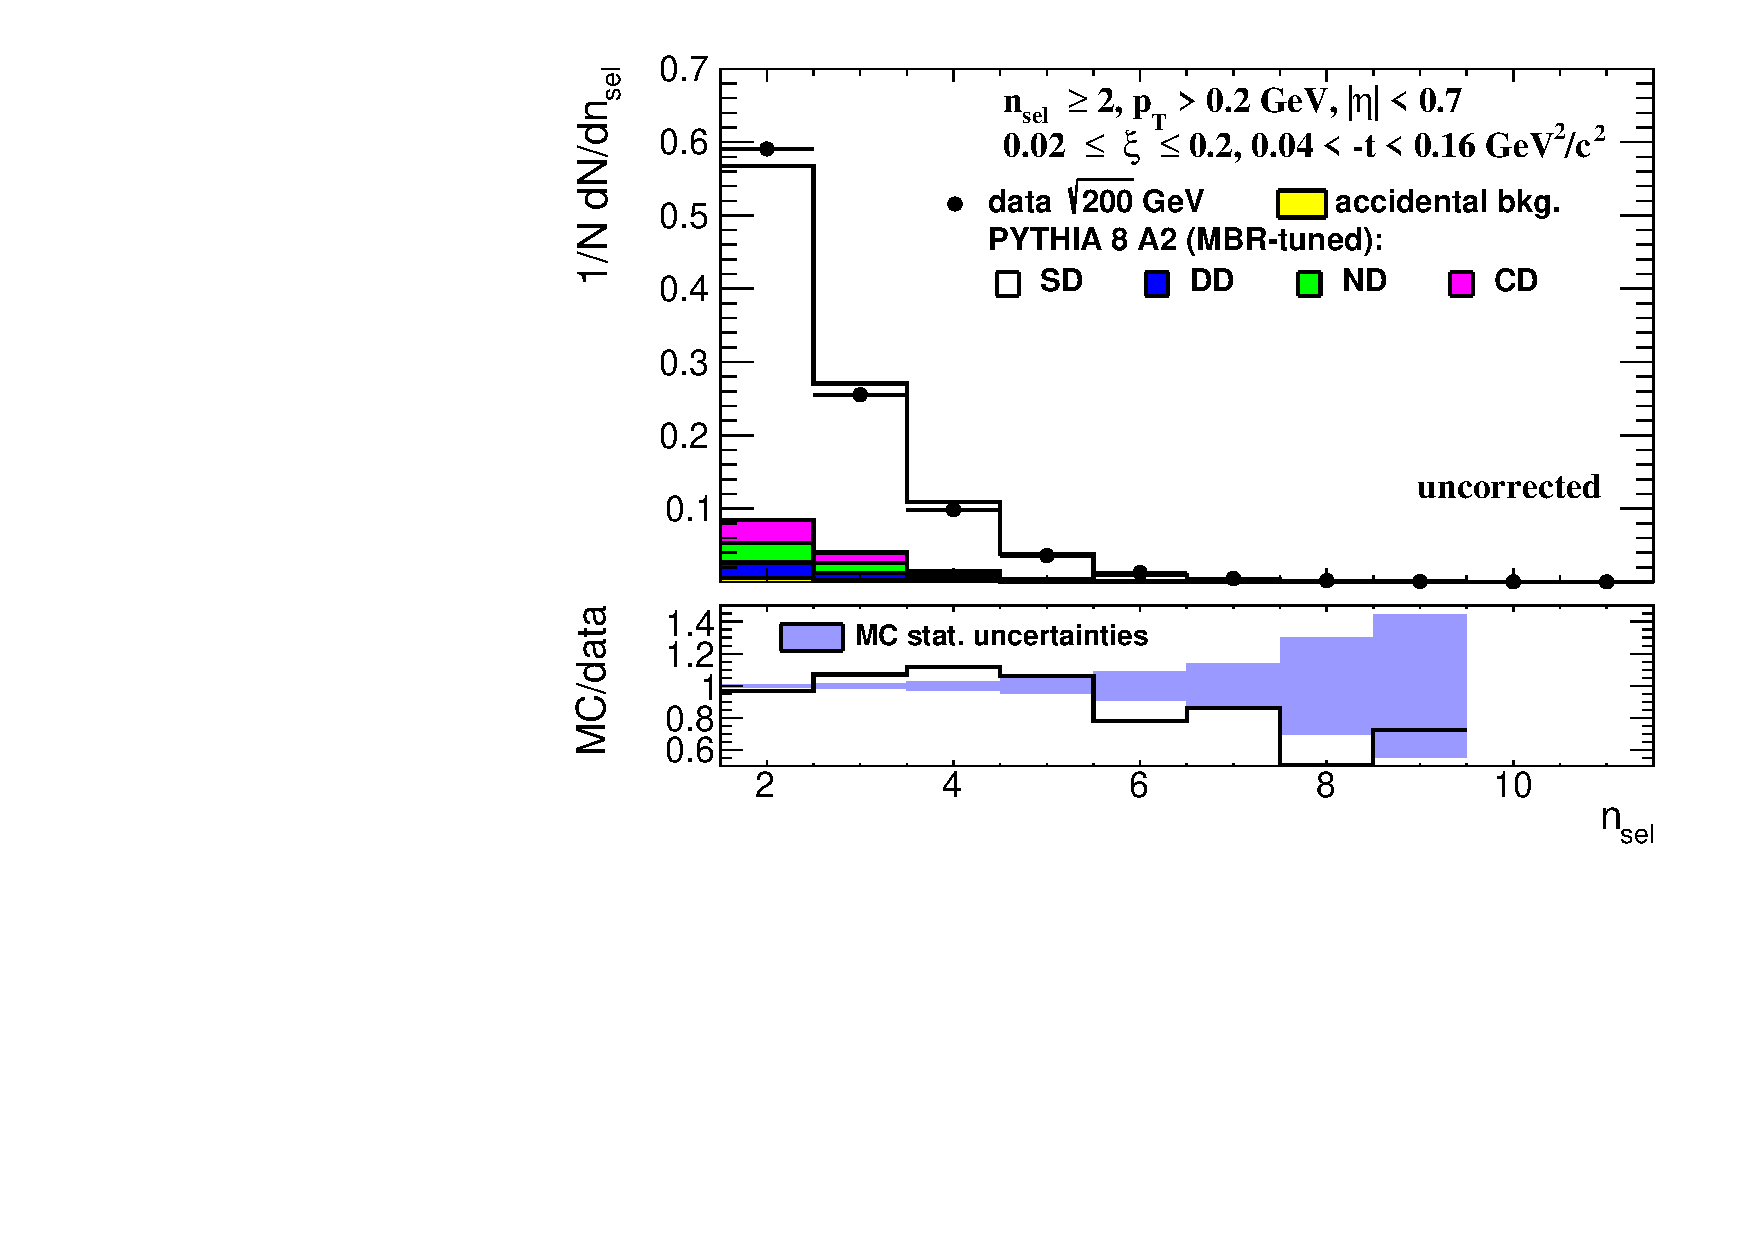
\includegraphics[width=\linewidth, page=1]{chapters/chrgSTAR/img/nonSD/chrg/SDT_pythia_xi0_option2_RP_starsim_nsel.pdf}
	\end{subfigure}
	\begin{subfigure}{.49\textwidth}
		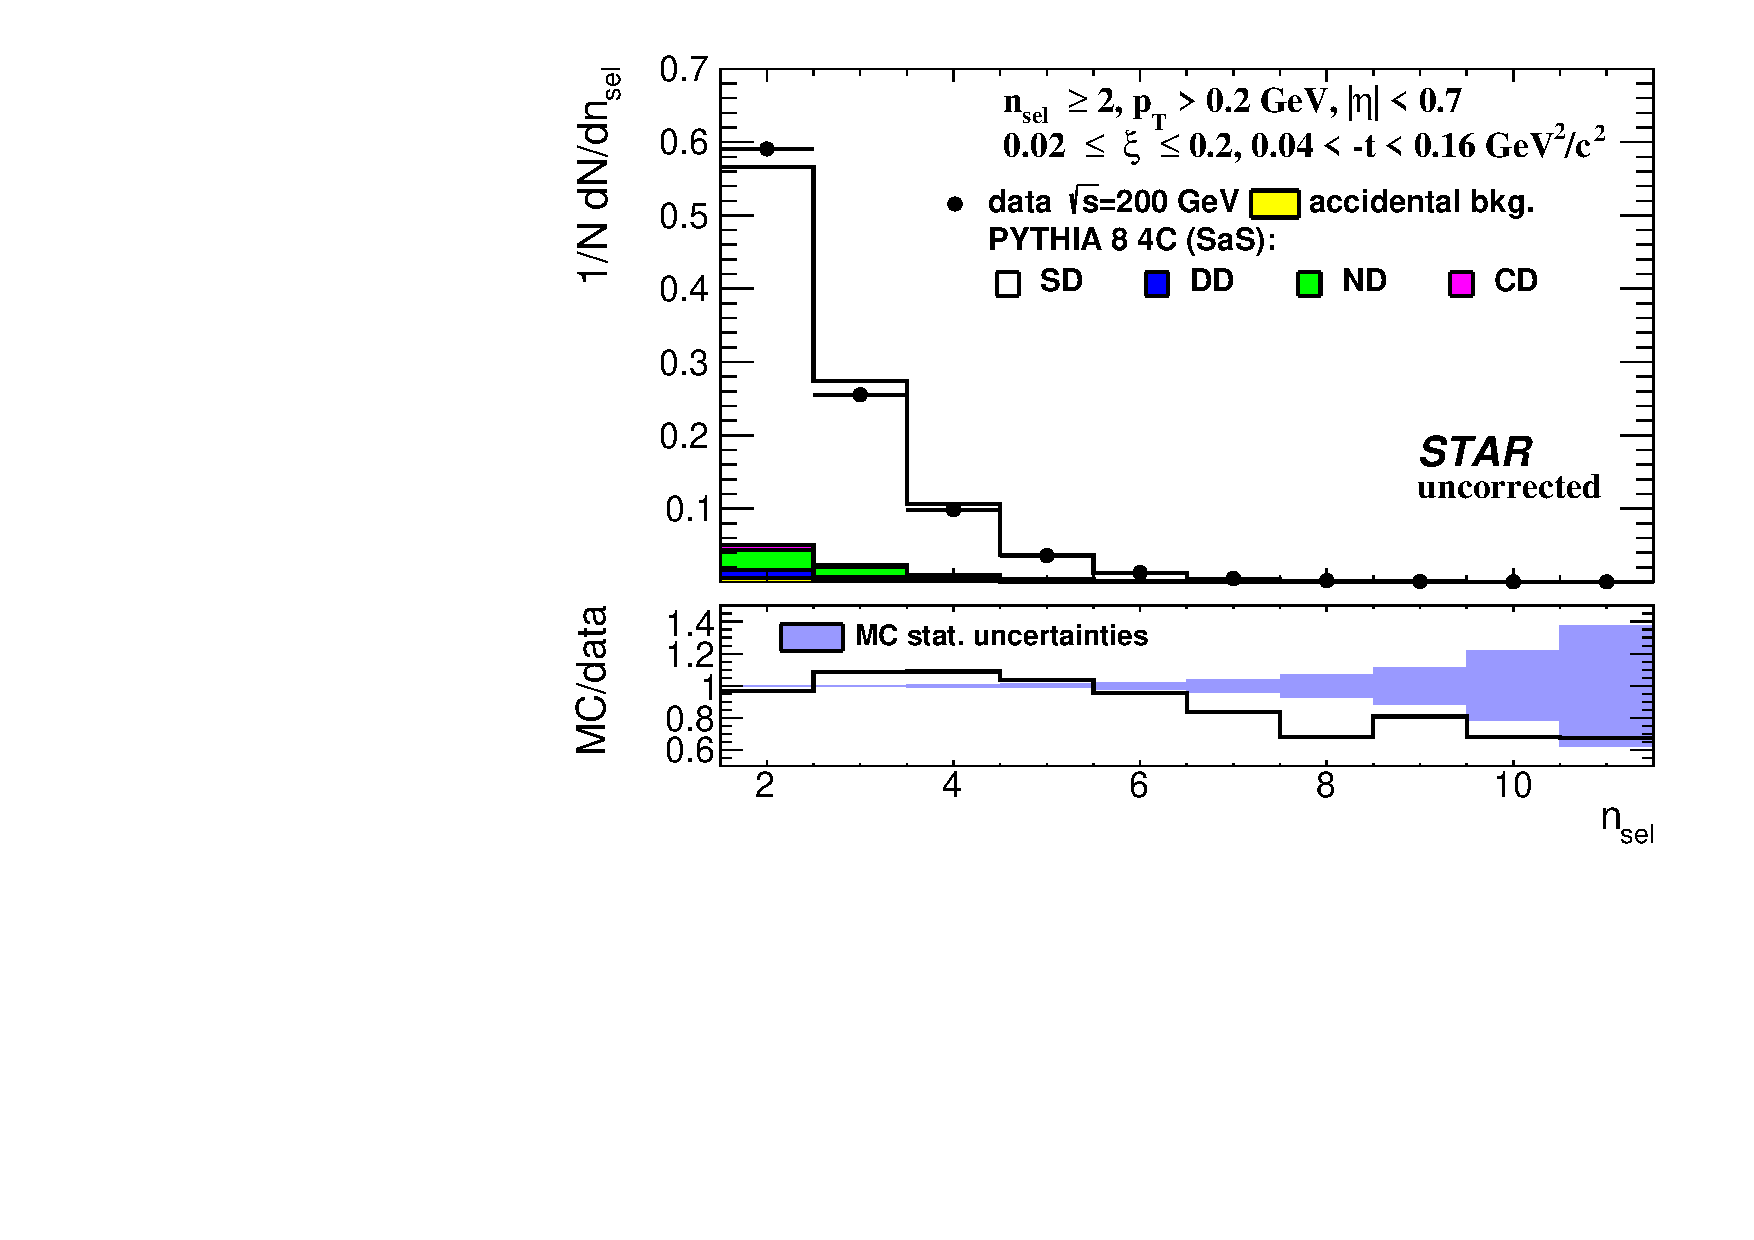
\includegraphics[width=\linewidth, page=1]{chapters/chrgSTAR/img/nonSD/SDT_pythia_xi0_sas_RP_starsim_nsel.pdf}
	\end{subfigure}
	\begin{subfigure}{.49\textwidth}
		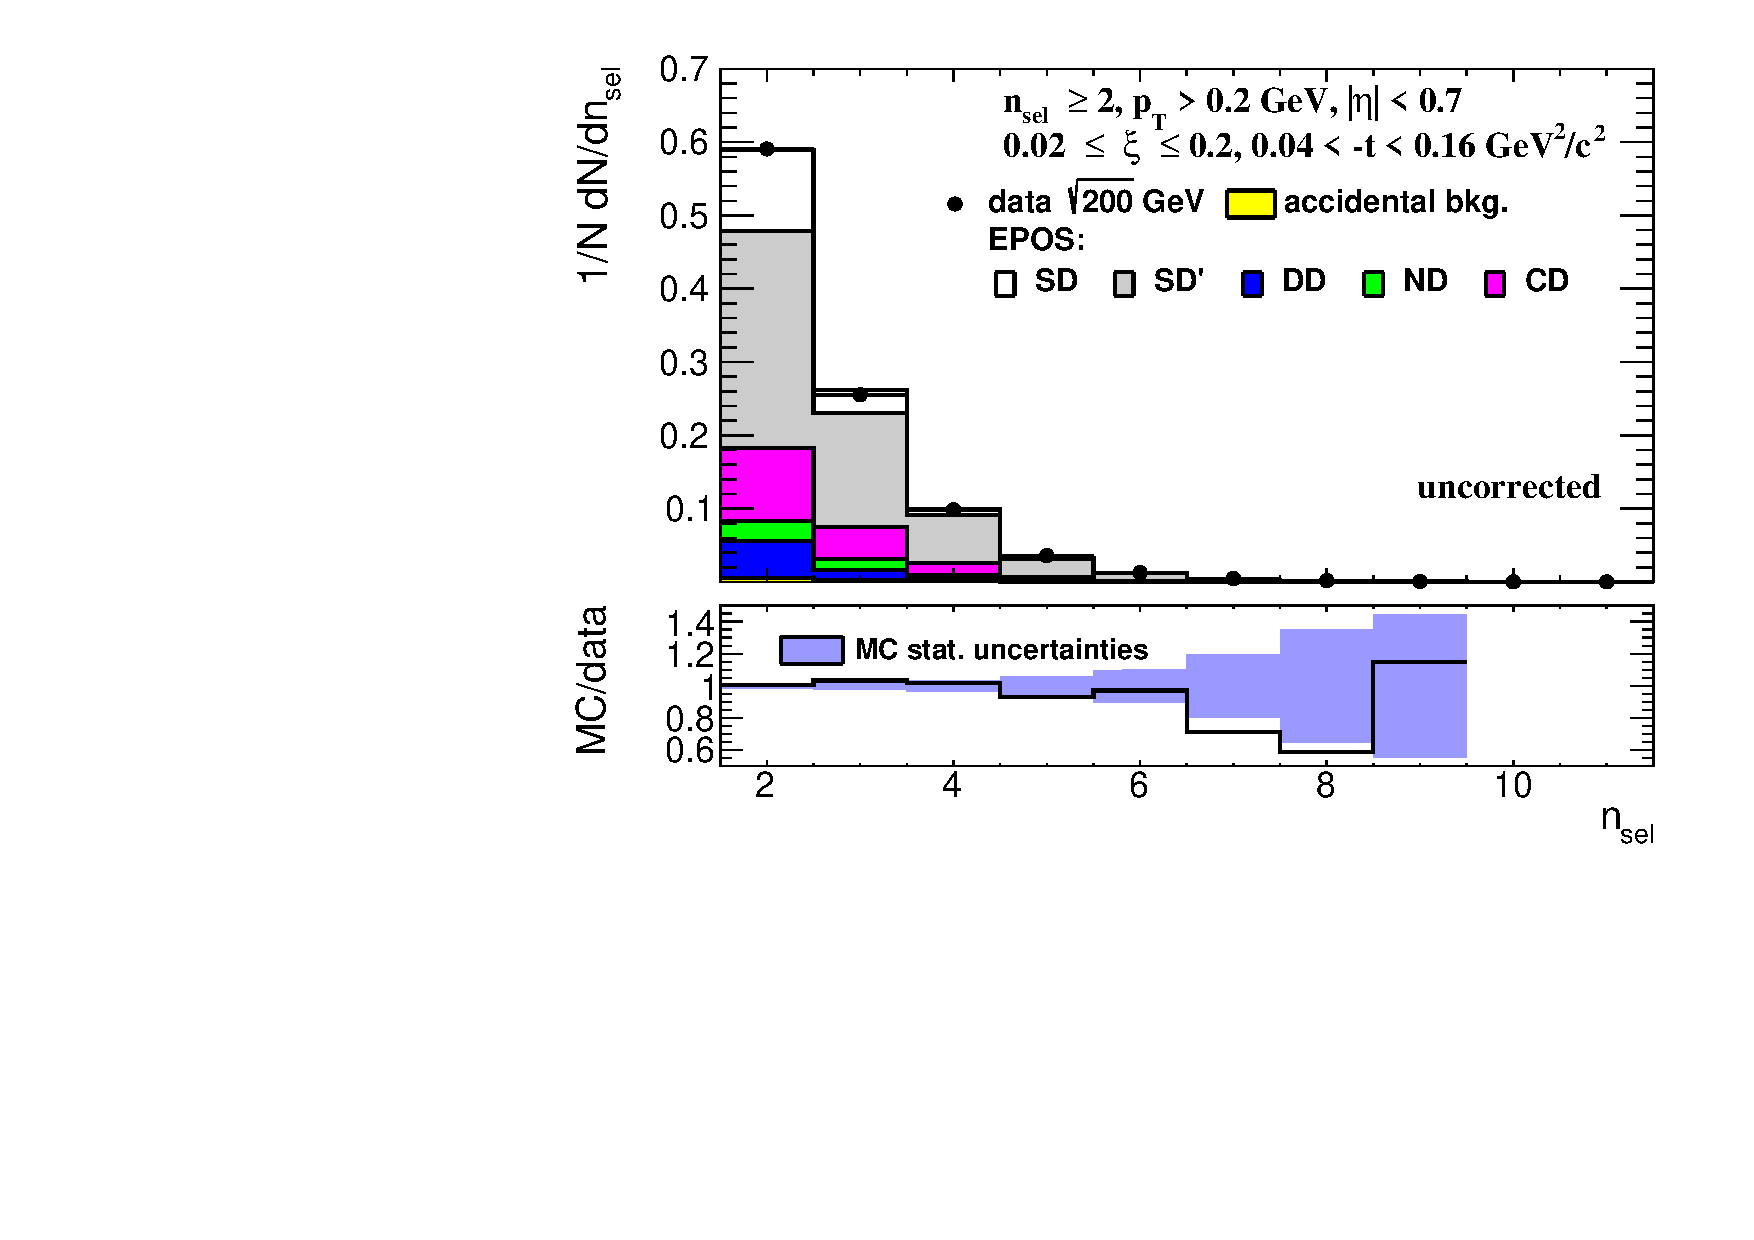
\includegraphics[width=\linewidth, page=1]{chapters/chrgSTAR/img/nonSD/chrg/SDT_epos_xi0_RP_starsim_nsel.pdf}
	\end{subfigure}
	%\begin{minipage}{.49\textwidth}
	\caption{Uncorrected distributions of data compared to various MC models: (top left) PYTHIA~8 A2 (MBR), (top right) PYTHIA~8 A2 (MBR-tuned), (bottom left) PYTHIA~8 4C (SaS) and (bottom right) EPOS, as a function of $n_{\mathrm{sel}}$. The~ratio of MC predictions and data is shown in the~bottom panels.}
	\label{fig:nonSDnsel}
	%\end{minipage}
	
%\end{figure}

%\begin{figure}[t!]
	%\vspace{-0.5cm}
	\centering
	\begin{subfigure}{.49\textwidth}
		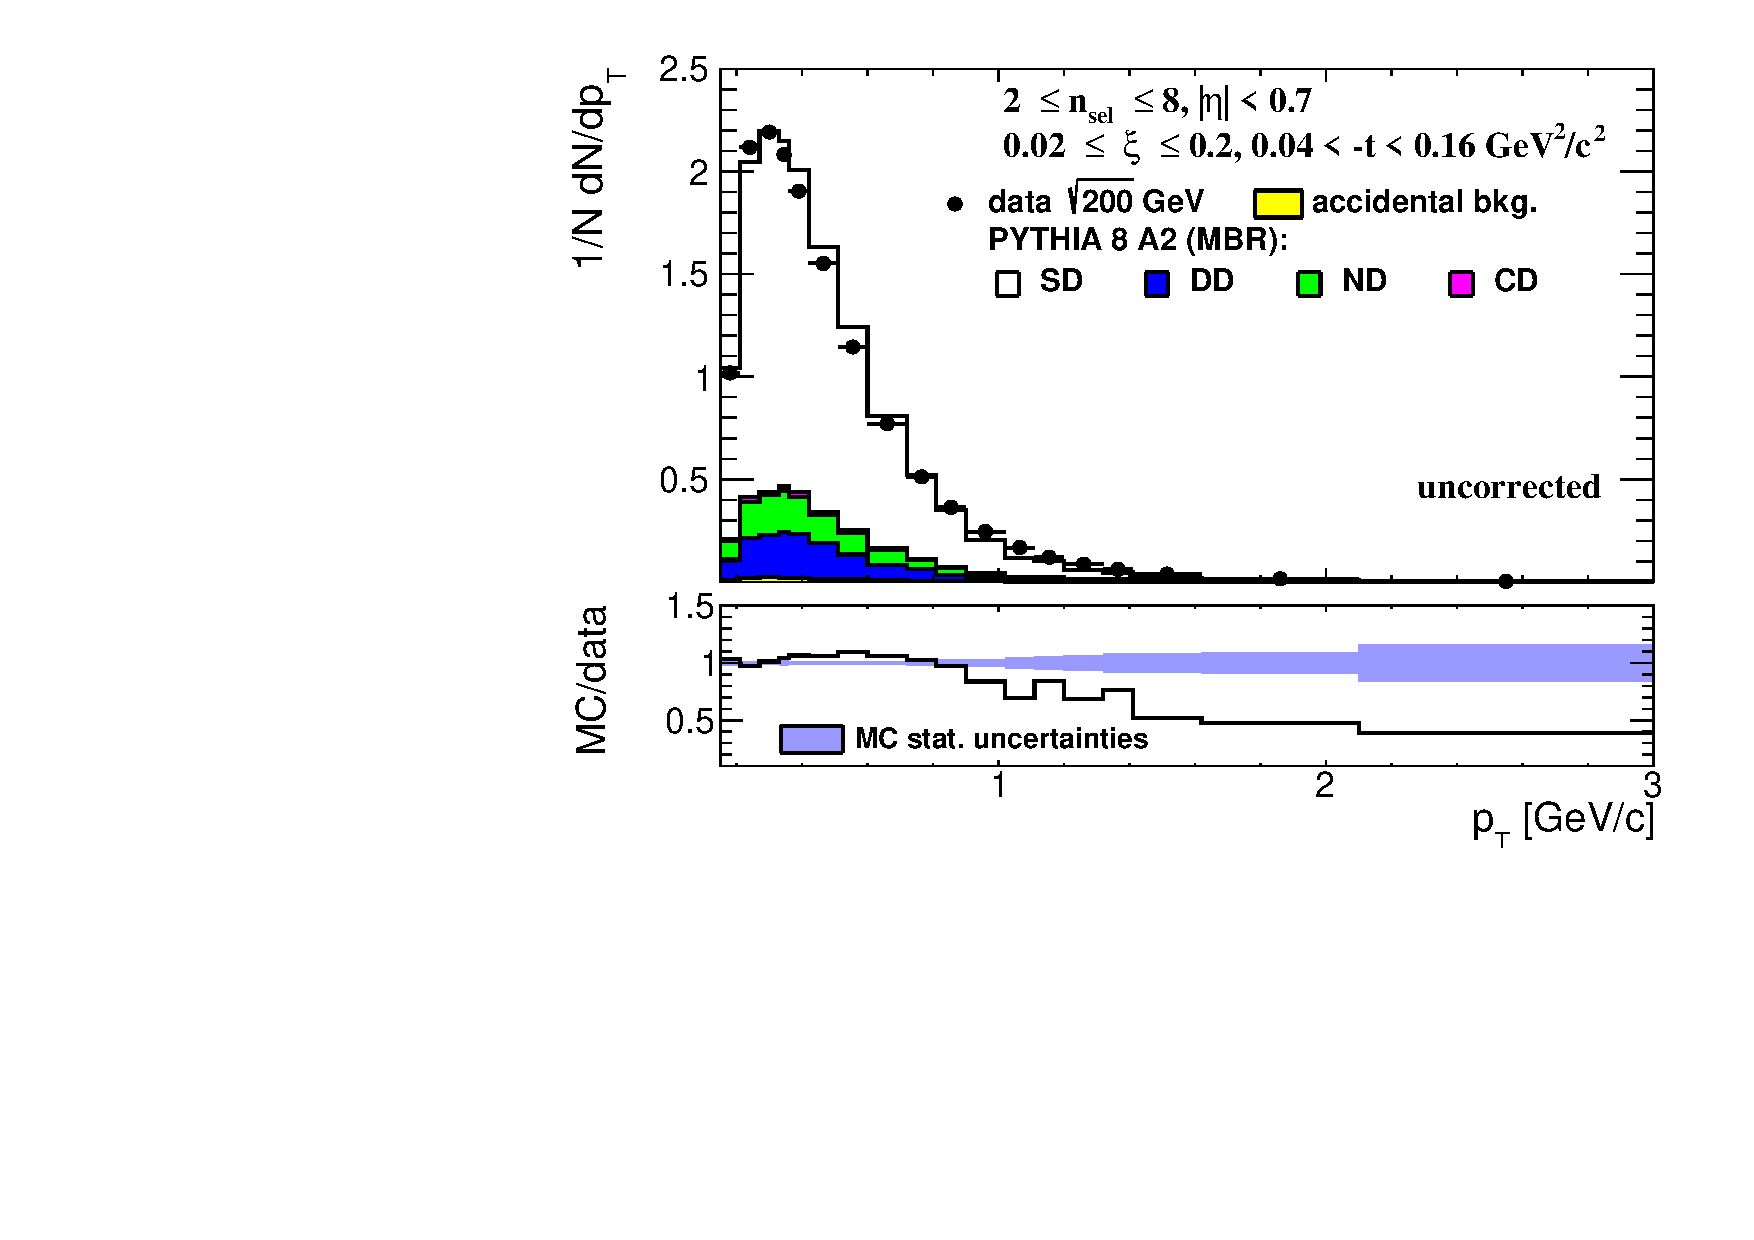
\includegraphics[width=\linewidth, page=1]{chapters/chrgSTAR/img/nonSD/chrg/SDT_pythia_xi0_RP_starsim_pt.pdf}
	\end{subfigure}
	\begin{subfigure}{.49\textwidth}
		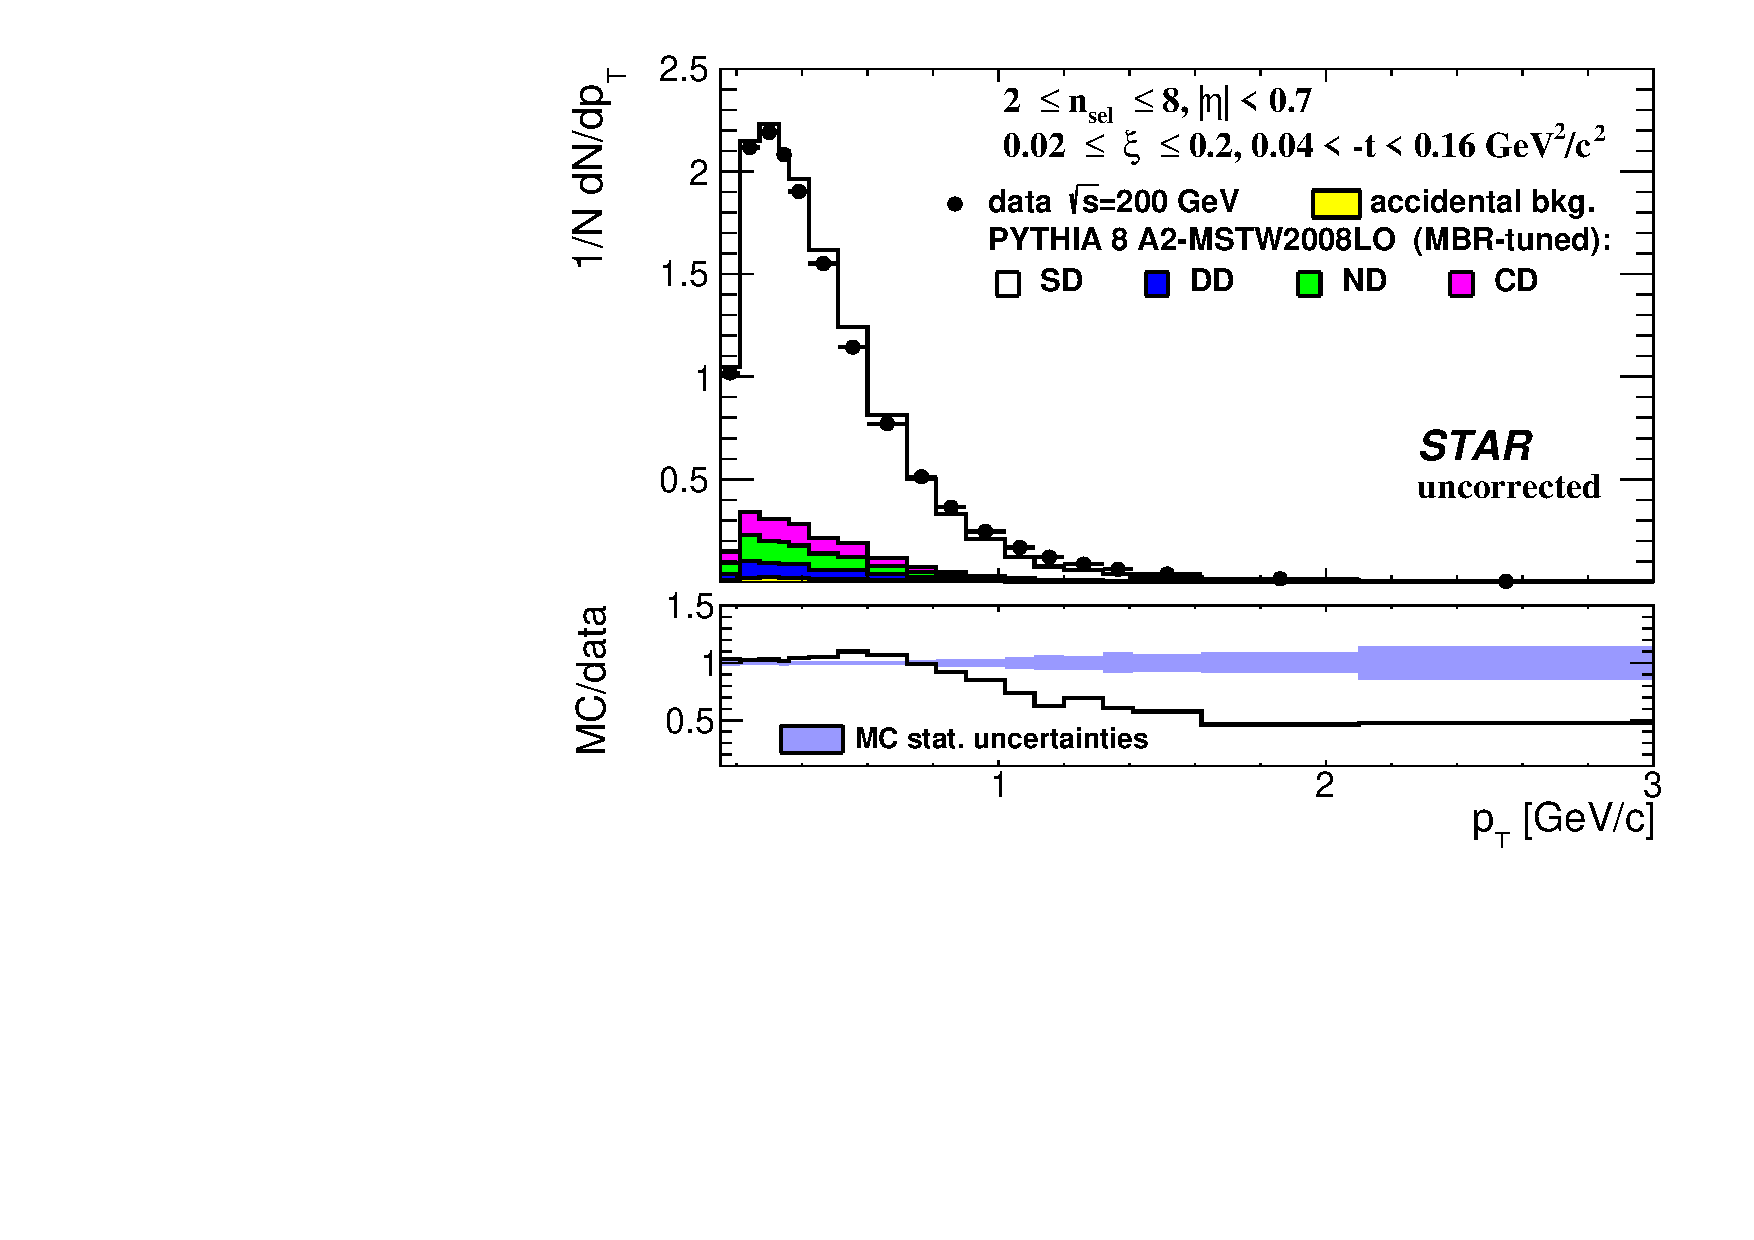
\includegraphics[width=\linewidth, page=1]{chapters/chrgSTAR/img/nonSD/chrg/SDT_pythia_xi0_option2_RP_starsim_pt.pdf}
	\end{subfigure}
	\begin{subfigure}{.49\textwidth}
		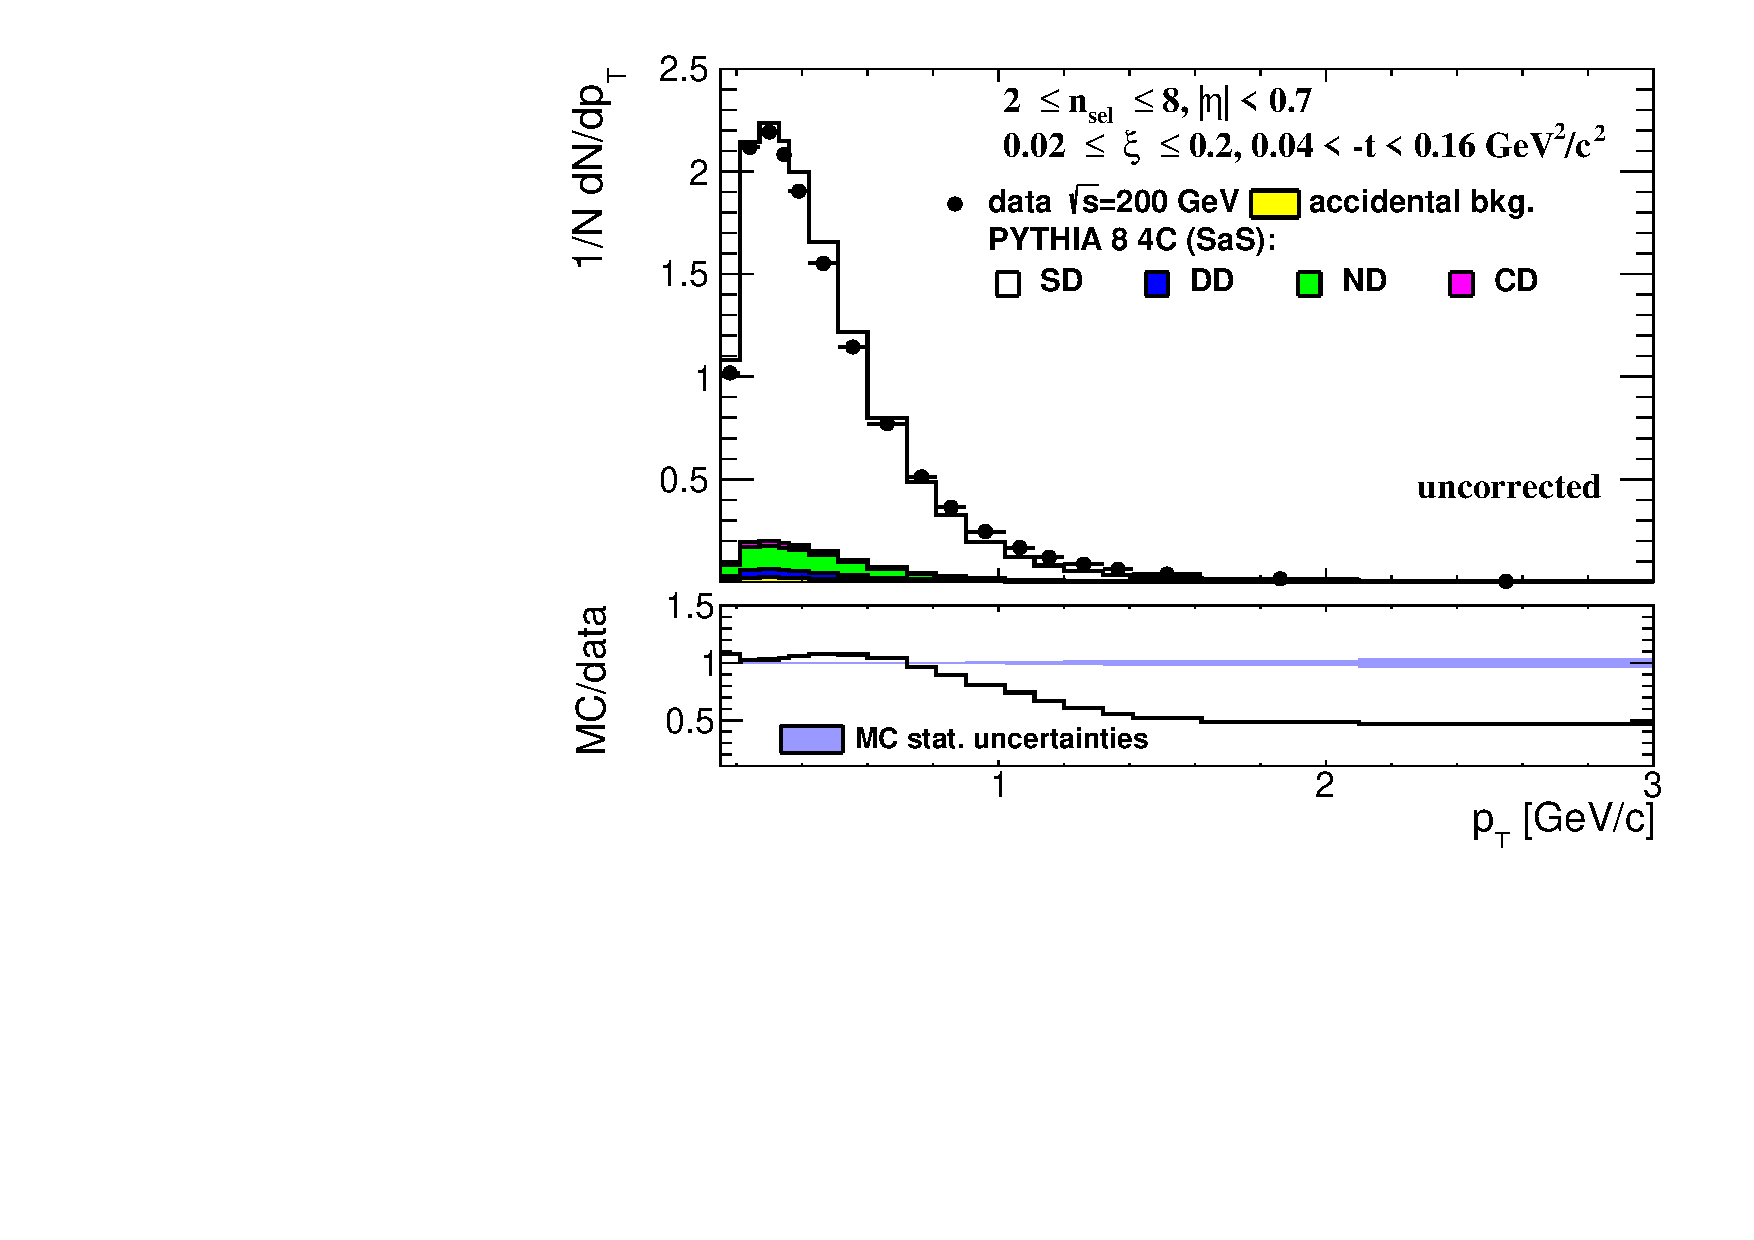
\includegraphics[width=\linewidth, page=1]{chapters/chrgSTAR/img/nonSD/SDT_pythia_xi0_sas_RP_starsim_pt.pdf}
	\end{subfigure}
	\begin{subfigure}{.49\textwidth}
		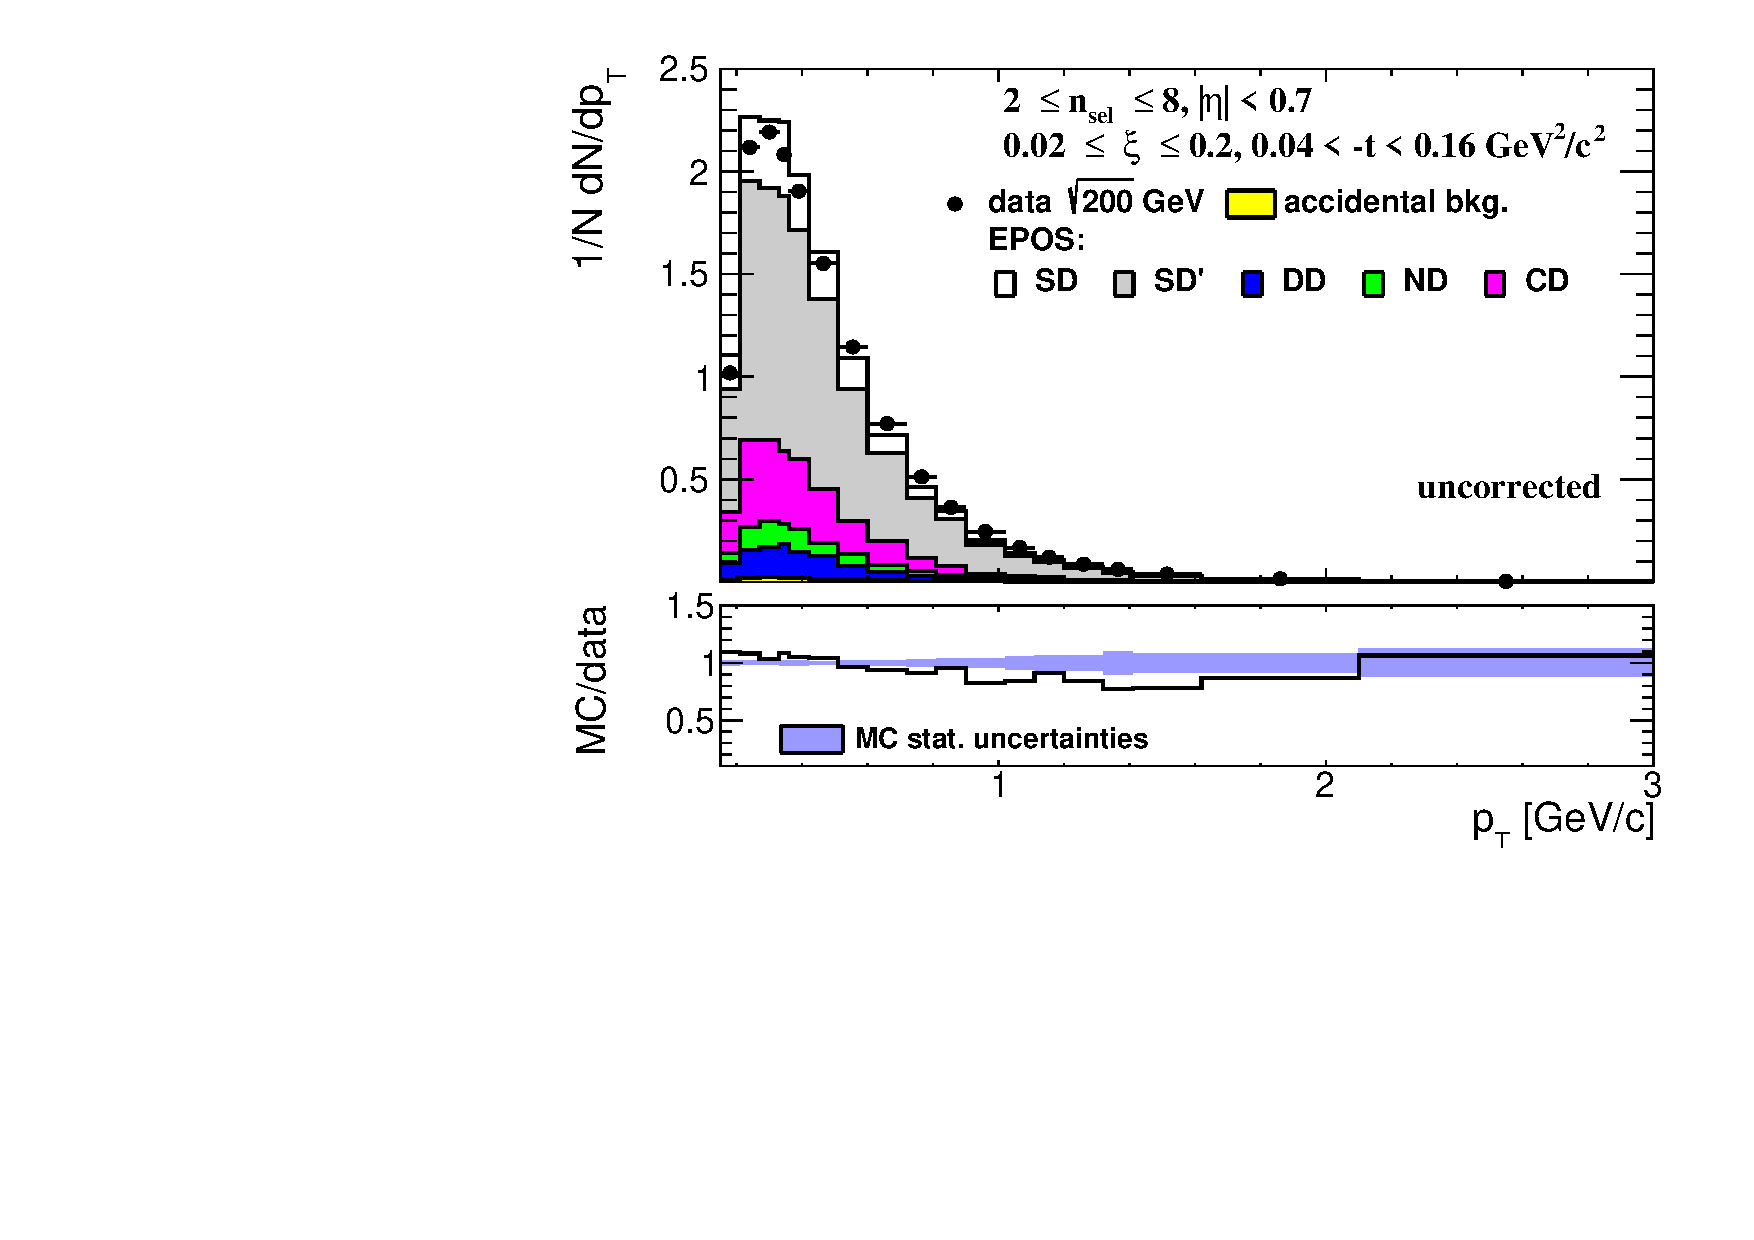
\includegraphics[width=\linewidth, page=1]{chapters/chrgSTAR/img/nonSD/chrg/SDT_epos_xi0_RP_starsim_pt.pdf}
	\end{subfigure}
	%\begin{minipage}{.49\textwidth}
		\caption{Uncorrected distributions of data compared to various MC models: (top left) PYTHIA~8 A2 (MBR), (top right) PYTHIA~8 A2 (MBR-tuned), (bottom left) PYTHIA~8 4C (SaS) and (bottom right) EPOS, as a function of $p_{\mathrm{T}}$. The~ratio of MC predictions and data is shown in the~bottom panels.}
		\label{fig:nonSDpt}
	%\end{minipage}
	%\vspace{-0.5cm}
\end{figure}
%\newpage
\begin{figure}[t!]
	%	\vspace{-0.5cm}
	\thisfloatpagestyle{fancy}
	\centering
	\begin{subfigure}{.49\textwidth}
		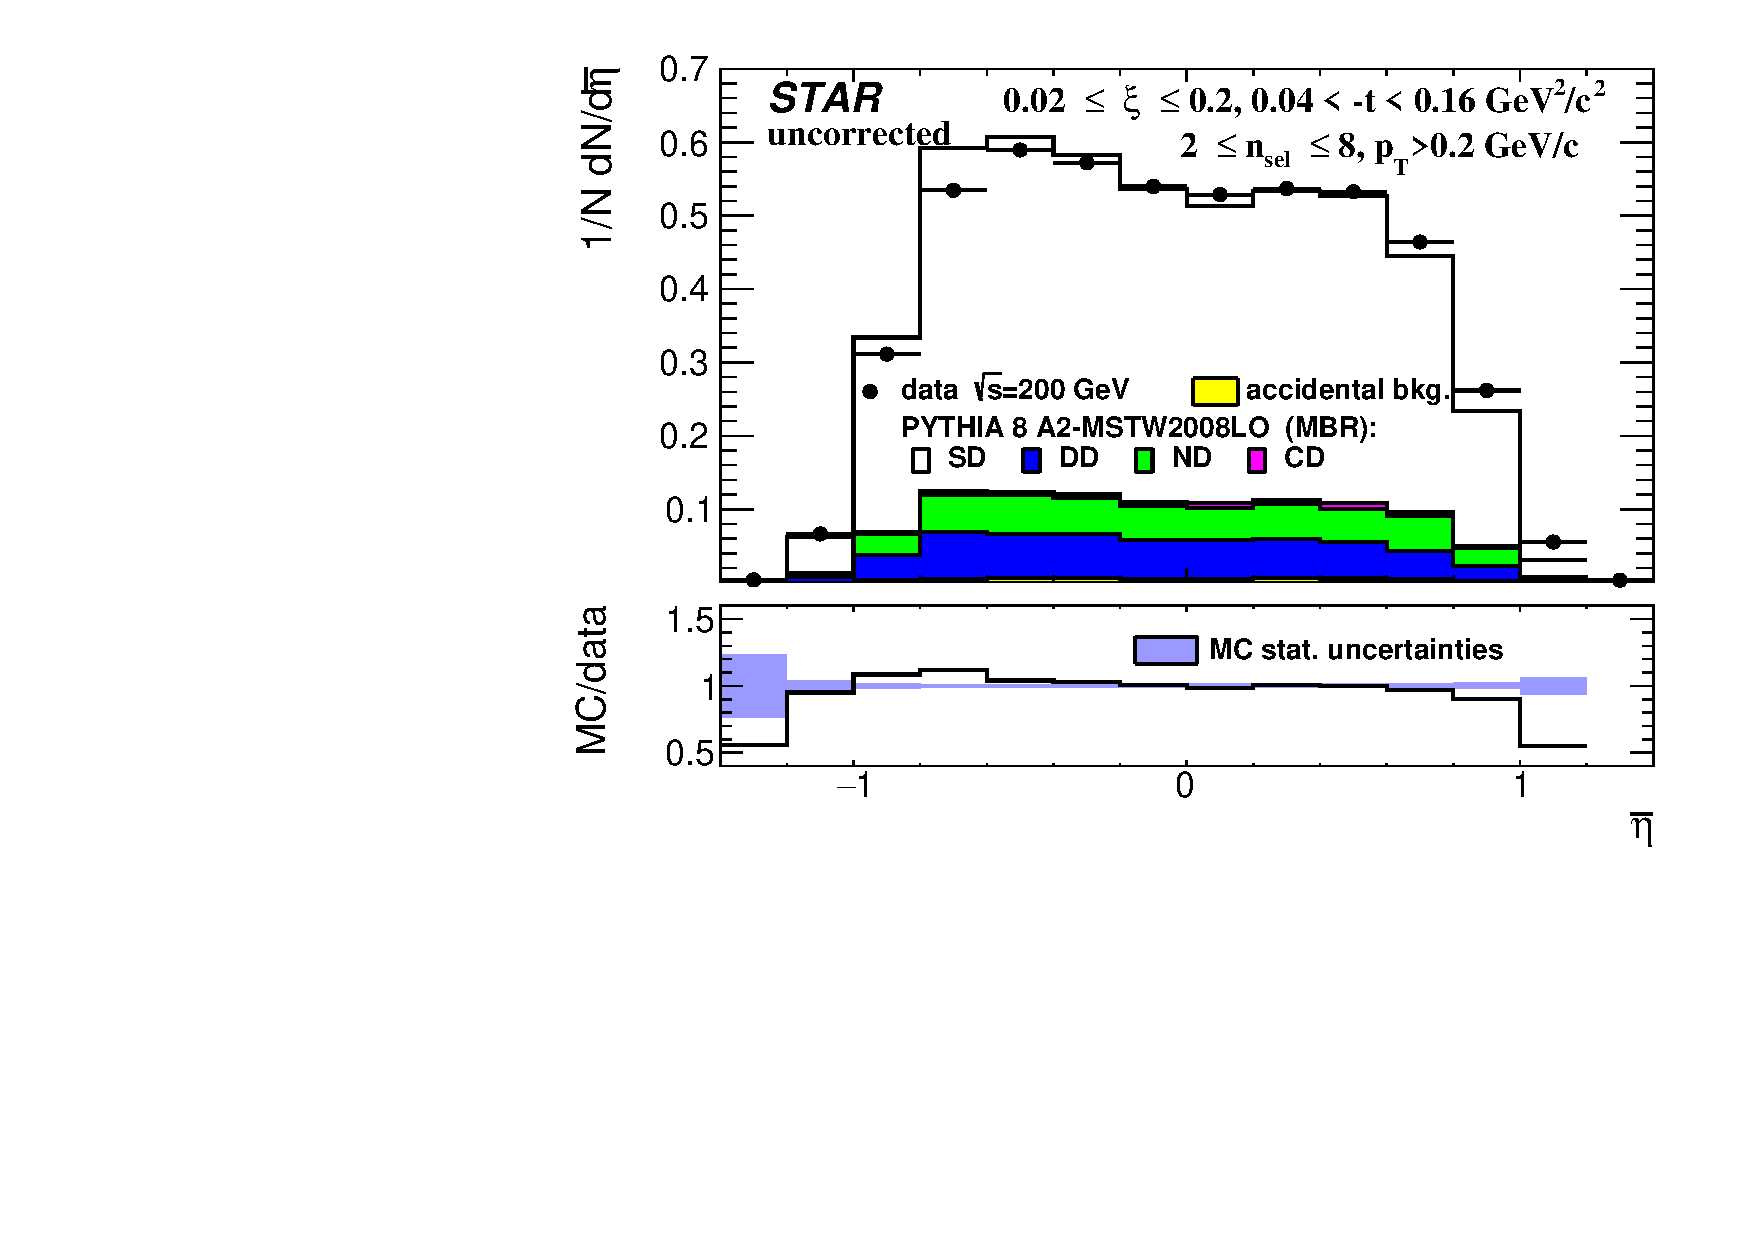
\includegraphics[width=\linewidth, page=1]{chapters/chrgSTAR/img/nonSD/chrg/SDT_pythia_xi0_RP_starsim_eta.pdf}
	\end{subfigure}
	\begin{subfigure}{.49\textwidth}
		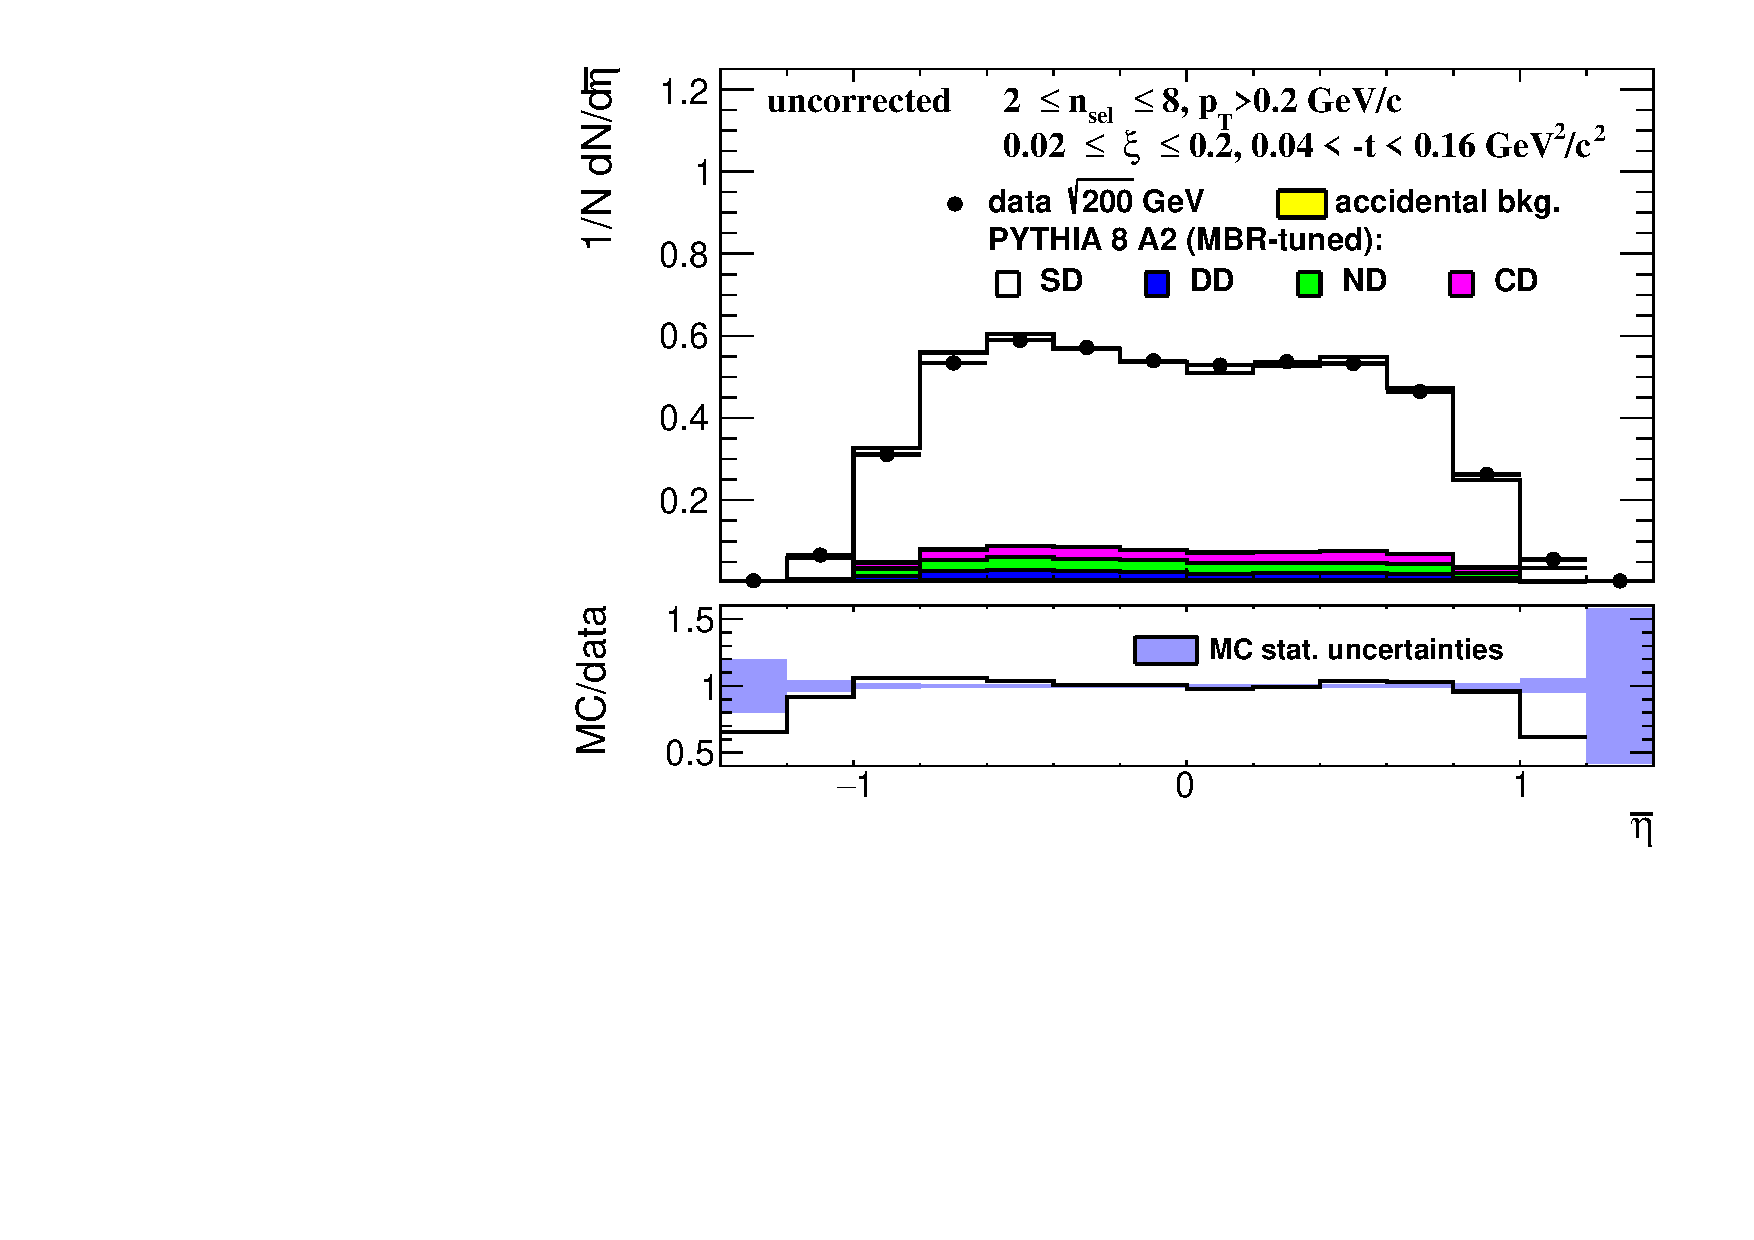
\includegraphics[width=\linewidth, page=1]{chapters/chrgSTAR/img/nonSD/chrg/SDT_pythia_xi0_option2_RP_starsim_eta.pdf}
	\end{subfigure}
	\begin{subfigure}{.49\textwidth}
		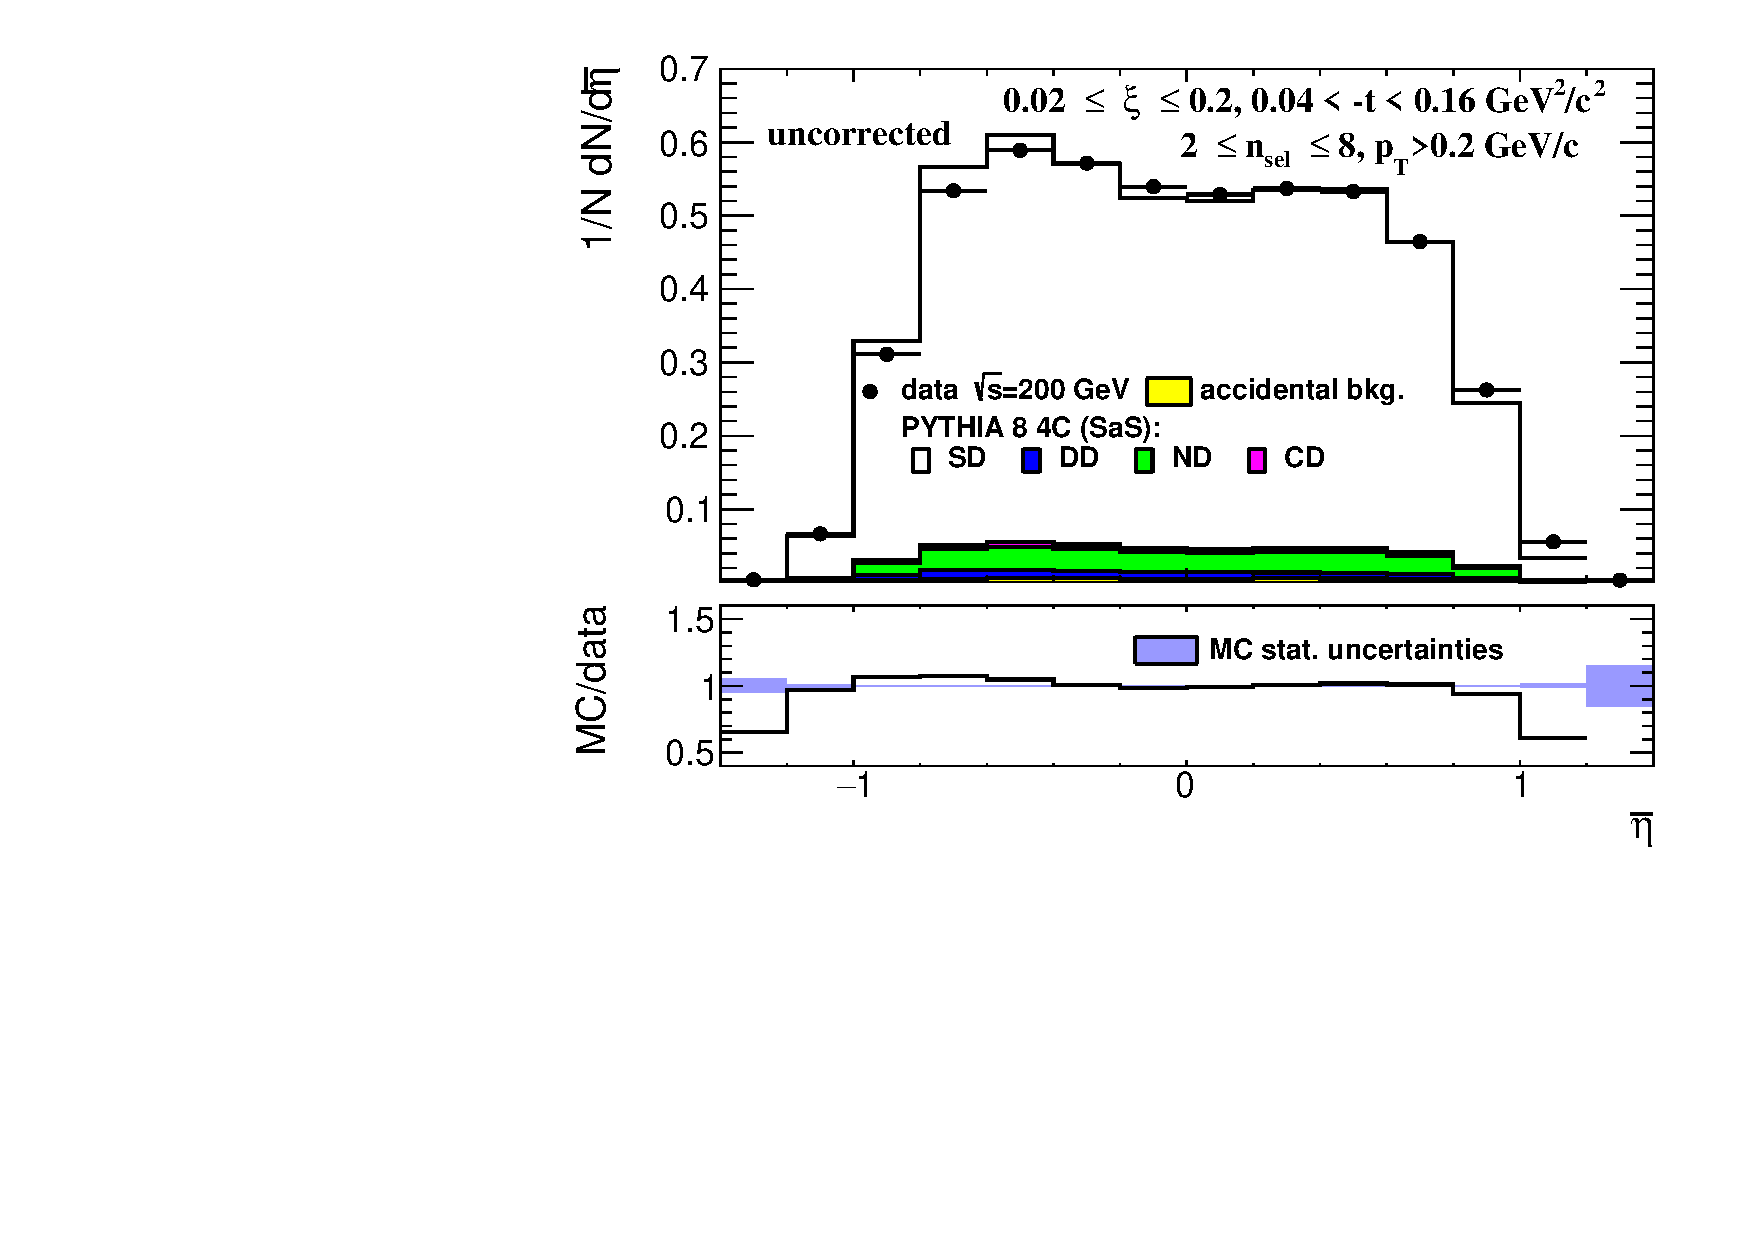
\includegraphics[width=\linewidth, page=1]{chapters/chrgSTAR/img/nonSD/SDT_pythia_xi0_sas_RP_starsim_eta.pdf}
	\end{subfigure}
	\begin{subfigure}{.49\textwidth}
		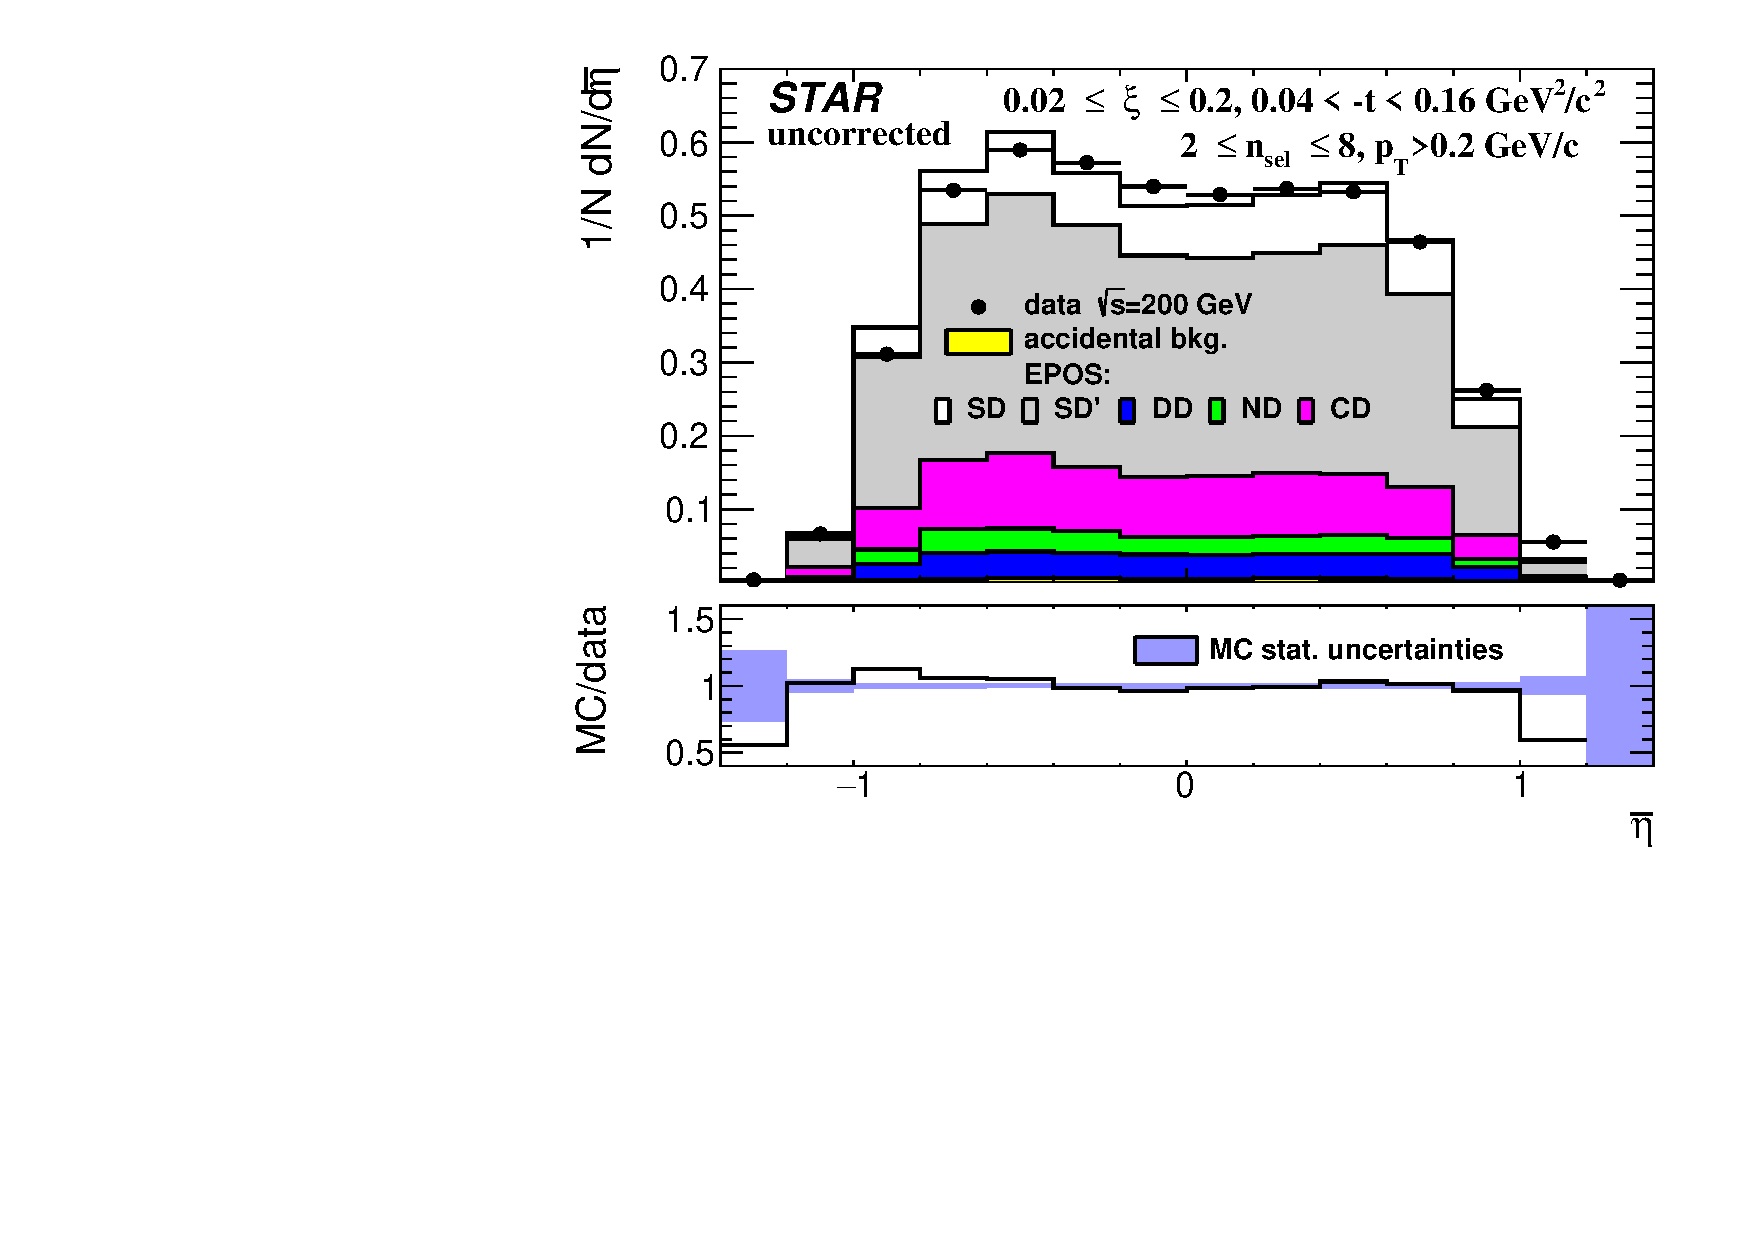
\includegraphics[width=\linewidth, page=1]{chapters/chrgSTAR/img/nonSD/chrg/SDT_epos_xi0_RP_starsim_eta.pdf}
	\end{subfigure}
	%\begin{minipage}{.49\textwidth}
		\caption{Uncorrected distributions of data compared to various MC models: (top left) PYTHIA~8 A2 (MBR), (top right) PYTHIA~8 A2 (MBR-tuned), (bottom left) PYTHIA~8 4C (SaS) and (bottom right) EPOS, as a function of $\bar{\eta}$. The~ratio of MC predictions and data is shown in the~bottom panels.}
		\label{fig:nonSDera}
	%\end{minipage}
	
\end{figure}
%\end{comment}
%\FloatBarrier
%background non primary
\section{Background from Non-Primary Tracks}\label{section:star_background_primary}
Reconstructed tracks matched to a~non-primary particle, so-called background tracks,  originate  mainly from the~following sources:
\begin{itemize}
	\item decays of short-lived primary particles with strange quark content (mostly $K^0$, $\Lambda^0$),
	\item photons from $\pi^0$ and $\eta$ decays which are converting to $e^+e^-$,
	\item hadronic interactions of particles with the beam-pipe or detector dead material.
\end{itemize} 

\begin{figure}[b!]
	\centering
	\begin{subfigure}{.49\textwidth}
		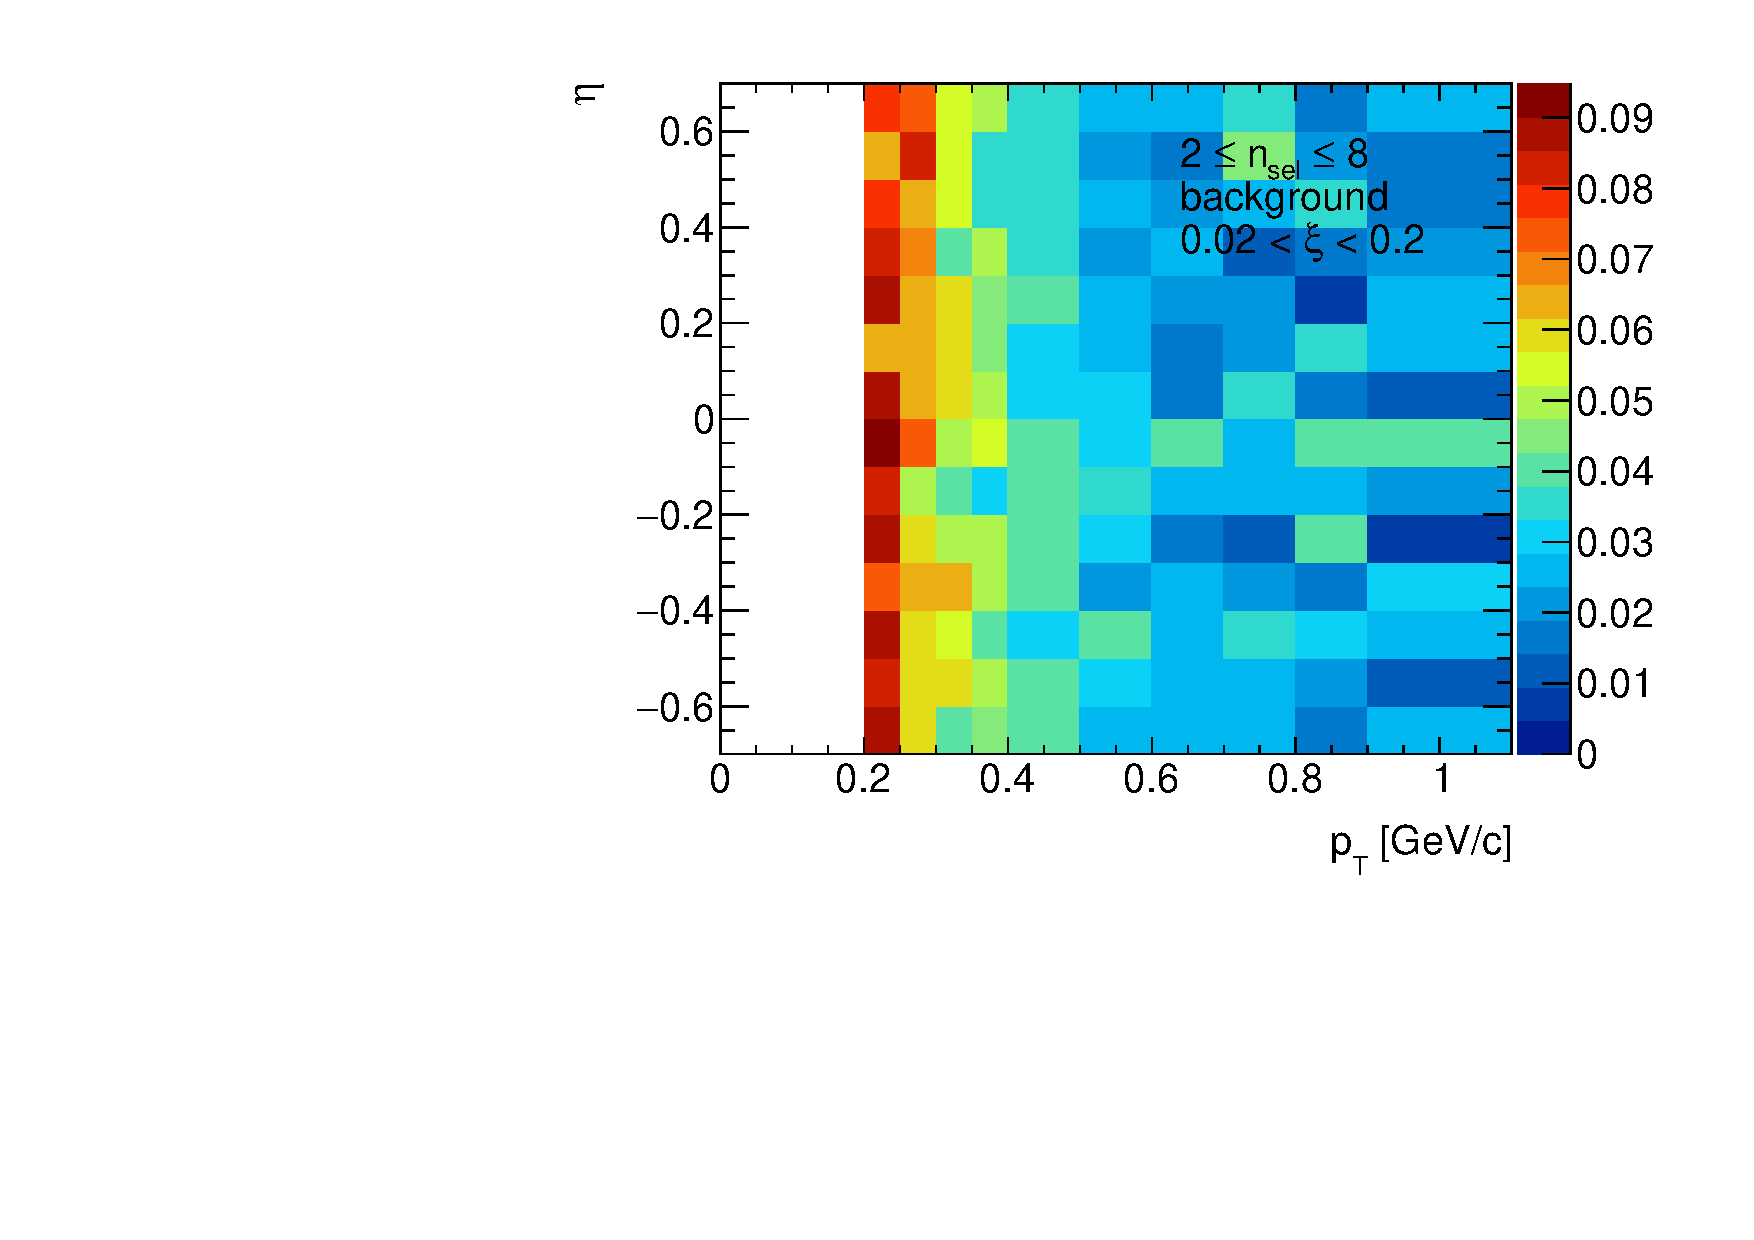
\includegraphics[width=\linewidth, page=1]{chapters/chrgSTAR/img/chargedBkg/bkg2D.pdf}
	\end{subfigure}
	\begin{subfigure}{.49\textwidth}
		\includegraphics[width=\linewidth, page=7]{chapters/chrgSTAR/img/chargedBkg/bkg2D_epos.pdf}
	\end{subfigure}
	\begin{comment}
	\begin{subfigure}{.45\textwidth}
	\includegraphics[width=\linewidth, page=4]{chapters/chrgSTAR/img/chargedBkg/bkg2D.pdf}
	\end{subfigure}
	\begin{subfigure}{.45\textwidth}
	\includegraphics[width=\linewidth, page=5]{chapters/chrgSTAR/img/chargedBkg/bkg2D.pdf}
	\end{subfigure}
	\end{comment}
	\caption{Distribution of fraction of selected tracks  associated with non-primary particles  in the~range $0.02<\xi<0.2$ as predicted by (left) PYTHIA~8 4C (SaS) embedding and (right) EPOS SD+SD$^\prime$.}
	\label{fig:bkg_fake_charged}
\end{figure}
Figure~\ref{fig:bkg_fake_charged} (left) shows the background from non-primary tracks, $f_{\textrm{bkg}}\left(p_{\textrm{T}},\eta\right)$, %and fake track $f_{\textrm{fake}}\left(p_{\textrm{T}},\eta\right)$ contribution to reconstructed tracks 
as a~function of tracks' $p_{\textrm{T}}$ and $\eta$, predicted by PYTHIA~8 SD model. There were no differences observed in the~background contribution in different $\xi$ ranges, hence, all three $\xi$ ranges were merged for this study. The highest background fraction, which varies between $5-10\%$, was found to be at low $p_{\textrm{T}}$.  %Due to too low statistics in PYTHIA~8 embedding \ac{MC}, the~shape of the~fake track contribution was assumed to be the~same in all three $\xi$ ranges. However, its normalization was calculated for each $\xi$ range separately with a ratio between the ranges of $1: 0.74: 1.11$.


Figure~\ref{fig:bkg_fake_charged} (right) shows the~background track contribution to reconstructed tracks as a~function of $p_\textrm{T}$ and $\eta$ calculated from EPOS SD+SD$^\prime$. The differences between
PYTHIA~8 and EPOS, which are up to $50\%$ for $p_\textrm{T}>0.5$~GeV/c (as shown in Fig.~\ref{fig:bkg_epos_charged_1D}), were symmetrized and taken as a~systematic uncertainty.

There is also a~small ($<0.5\%$) contribution from fake tracks, $f_{\textrm{fake}}\left(p_{\textrm{T}},\eta\right)$, i.e. tracks not associated with true-level particles, coming from out-of-time pile-up or  formed by a~random combination of TPC hits. The~change by $\pm100\%$ in this contribution was taken as a systematic uncertainty.

\begin{figure}[t!]
	\centering
	\begin{subfigure}{.49\textwidth}
		\includegraphics[width=\linewidth, page=8]{chapters/chrgSTAR/img/chargedBkg/bkg2D.pdf}
	\end{subfigure}
	\begin{subfigure}{.49\textwidth}
		\includegraphics[width=\linewidth, page=9]{chapters/chrgSTAR/img/chargedBkg/bkg2D.pdf}
	\end{subfigure}
	\vspace{-0.25cm}
	\caption{PYTHIA~8 SD and EPOS SD+SD$^\prime$ predictions of fraction of selected tracks  associated with non-primary particles  as a~function of (left) $p_\textrm{T}$ and (right) $\eta$. The~ratio of EPOS and PYTHIA~8 predictions is shown in the~bottom panels.}
	\label{fig:bkg_epos_charged_1D}
	\vspace{-0.25cm}
\end{figure}

%\FloatBarrier
%background proton
\subsubsection{Proton Background}\label{section:star_background_proton}
Secondary particles can be created due to the interaction of particles with detector dead-material.
The proton sample contains background from such protons knocked out  from the~detector materials~\cite{STAR:spectra}. Most of these protons have large $\textrm{DCA}$ to the~primary vertex and are not associated with it. However, the~protons with small $\textrm{DCA}$  are included in the primary track sample. Antiprotons do not have knockout background, hence the~$\textrm{DCA}$ tail is almost absent in their $\textrm{DCA}$ distributions.

The fraction of knock-out background protons depends on a number of factors, including the~amount of detector material, analysis cuts and the $\xi$ of diffractive proton. While it is natural to calculate the fractions of primary and background protons in the~\ac{MC} sample, the \ac{MC} models do not necessarily predict the fraction of knock-out background protons without any bias. Hence,  data-driven methods should be used to calculate this type of background.

\begin{figure}[h!]
	\centering
	\begin{subfigure}{.49\textwidth}
		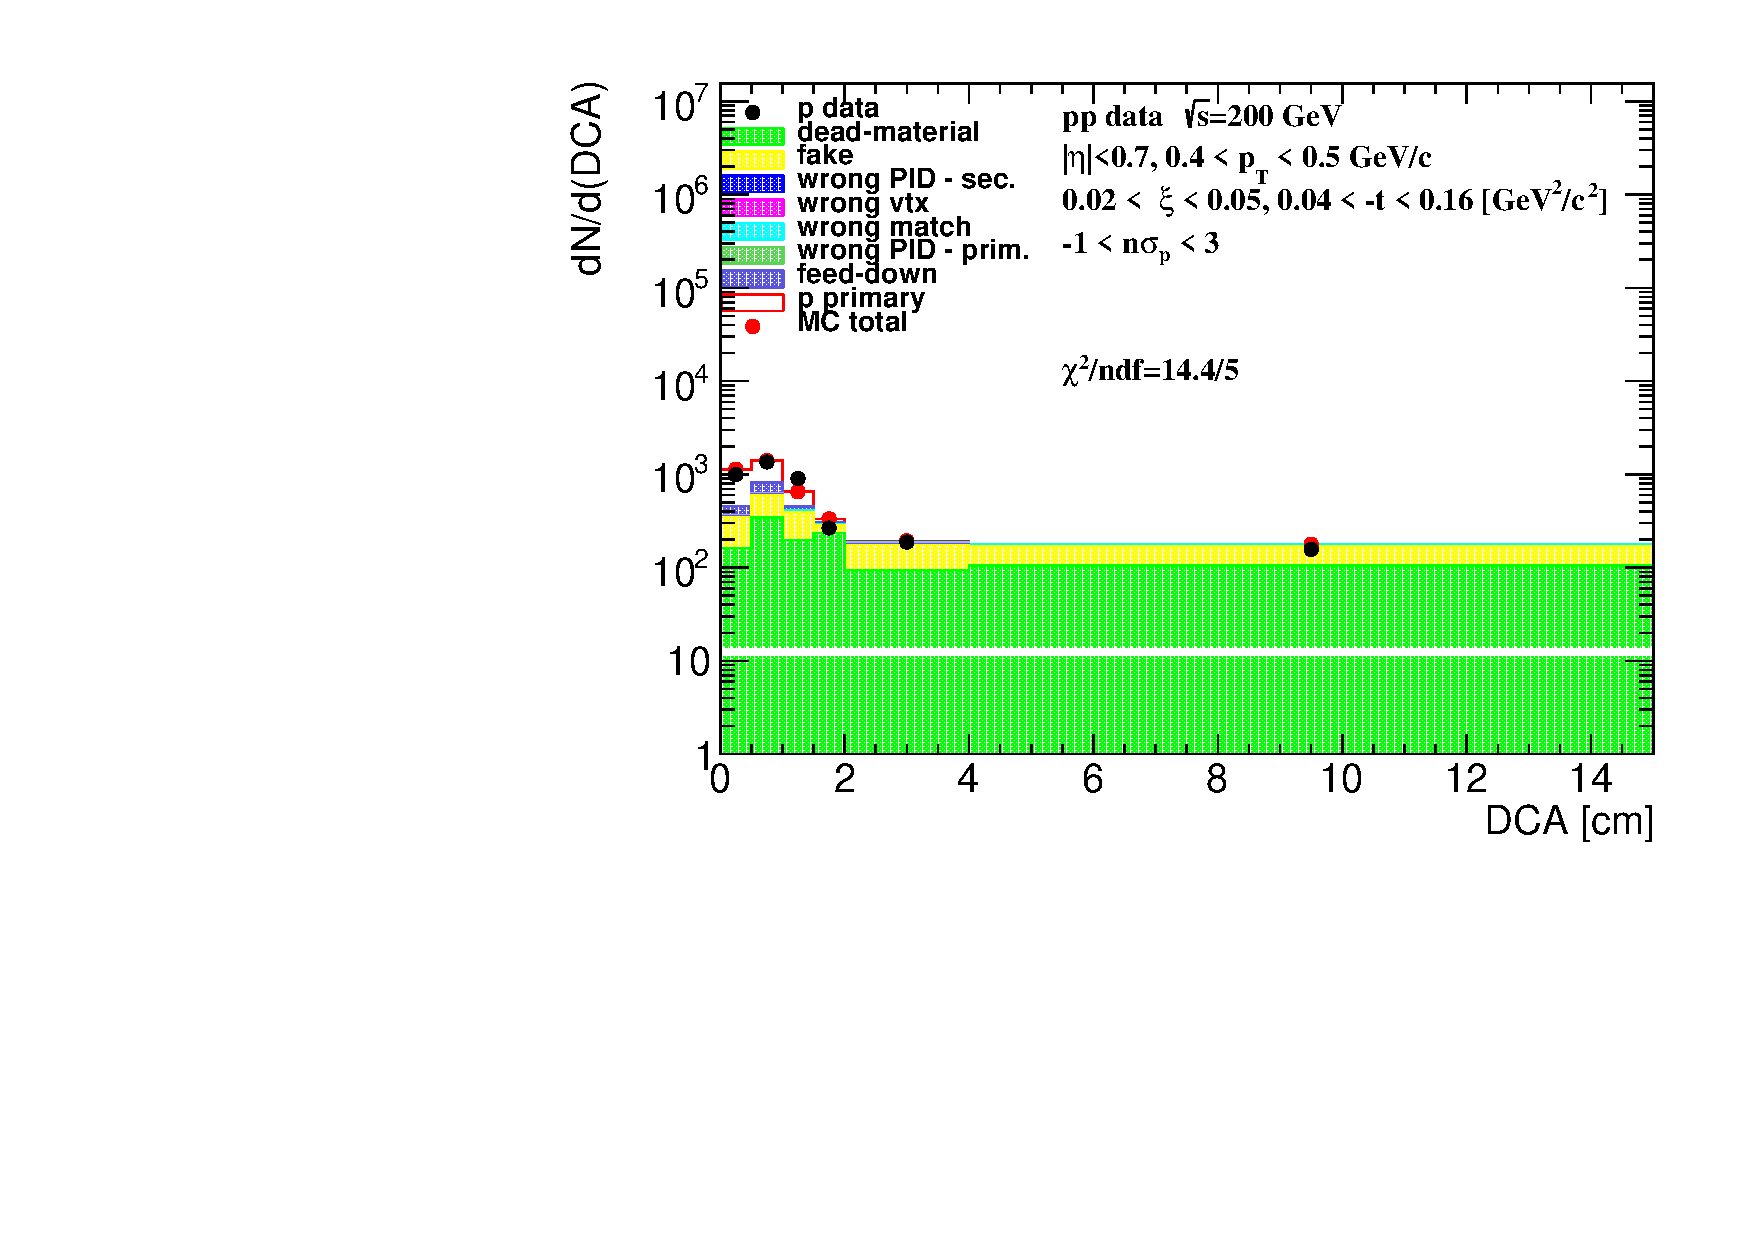
\includegraphics[width=\linewidth, page=1]{chapters/chrgSTAR/img/DCAproton/background_p_0.pdf}
	\end{subfigure}
	\begin{subfigure}{.49\textwidth}
		\includegraphics[width=\linewidth, page=2]{chapters/chrgSTAR/img/DCAproton/background_p_0.pdf}
	\end{subfigure}
	\begin{subfigure}{.49\textwidth}
		\includegraphics[width=\linewidth, page=3]{chapters/chrgSTAR/img/DCAproton/background_p_0.pdf}
	\end{subfigure}
	\begin{subfigure}{.49\textwidth}
		\includegraphics[width=\linewidth, page=4]{chapters/chrgSTAR/img/DCAproton/background_p_0.pdf}
	\end{subfigure}
	\caption{The $\textrm{DCA}$ distributions of protons for $0.4<p_T<0.5$~GeV/c shown for single range of $0.02<\xi<0.05$ (shown in log and linear scale in left and right column, respectively). The MC  contributions are shown after scaling the dead-material template  to the~tail of large $\textrm{DCA}$ values, $2<\textrm{DCA}<15$~cm. (top) Background enriched samples were used in the normalization procedure, whereas (bottom) the proton background was estimated from the nominal sample.}
	\label{fig:bkg_proton}
\end{figure}

In order to correct for the knock-out background protons, sample enriched in proton background  was used for background normalization, where $\textrm{DCA}_{xy}$, $\textrm{DCA}_z$ and $d_0$ cuts were abandoned. Additionally, at least one, instead of exactly one,  reconstructed vertex was allowed in this sample.  \Cref{fig:bkg_proton,fig:bkg_proton_bar} show the~$\textrm{DCA}$ distributions of protons and antiprotons, respectively, for  nominal (bottom) and background enriched (top) samples. The distributions for other $p_\textrm{T}$ and $\xi$ regions are shown in Appendix~\ref{appendix:DCA_proton}.
The protons and antiprotons are selected by a $dE/dx$ cut of $-1 < n\sigma_{p,\bar{p}} < 3$ where $n\sigma_{p,\bar{p}}$ is given by Eq.~\eqref{eq:nsigma}. In some $p_\textrm{T}$ regions, the~$dE/dx$ of (anti)protons and pions
starts to overlap, hence, the~asymmetric $n\sigma_{p,\bar{p}}$ cut was introduced in order to select as clean (anti)proton sample as possible.
The fraction of knock-out protons within the selected sample is determined via \ac{MC} template fits. The templates of reconstructed tracks with $dE/dx$ corresponding to the~proton and antiproton are obtained from PYTHIA~8 embedding \ac{MC} separately for:
\begin{itemize}
	\item primary (anti)protons,
	\item knock-out background protons (labeled as dead-material),
	\item fake tracks,
	\item secondary particles with $dE/dx$ of (anti)proton (labeled as wrong PID - sec.),
	\item tracks associated with primary (anti)protons, but with the reconstructed vertex  not matched to true-level primary vertex (labeled as wrong vtx),
	\item reconstructed track is partially matched to true-level particle (labeled as wrong match, track to true-level particle matching is described in~\cite{supplementaryNote}), i.e.  track and true-level particle have appropriate number of common hit points but the distance between true-level particle and track is too large, $\delta^2\left(\eta,\phi\right)>\left(0.15\right)^2$, thus, track is not considered as primary particle according to discussion in~\cite{supplementaryNote}, 
	\item primary particles with $dE/dx$ of (anti)proton (labeled as wrong PID - prim.),
	\item (anti)proton as a product of short-lived decays, mainly $\Lambda^0$ (labeled as feed-down).
\end{itemize}



First, the background enriched sample was analyzed  (Fig.~\ref{fig:bkg_proton}, top), where the template of knock-out background protons was normalized to the number of events in the fake-subtracted tail of the $\textrm{DCA}$ distribution, $2<\textrm{DCA}<15$~cm. Next the knock-out proton and fake background was subtracted from the $\textrm{DCA}$ distribution and the sum of other templates was normalized to the~number of events in the~signal region,  $\textrm{DCA}<1.5$~cm. 

\begin{figure}[h!]
	%\vspace{-1cm}
	\centering
	\begin{subfigure}{.49\textwidth}
		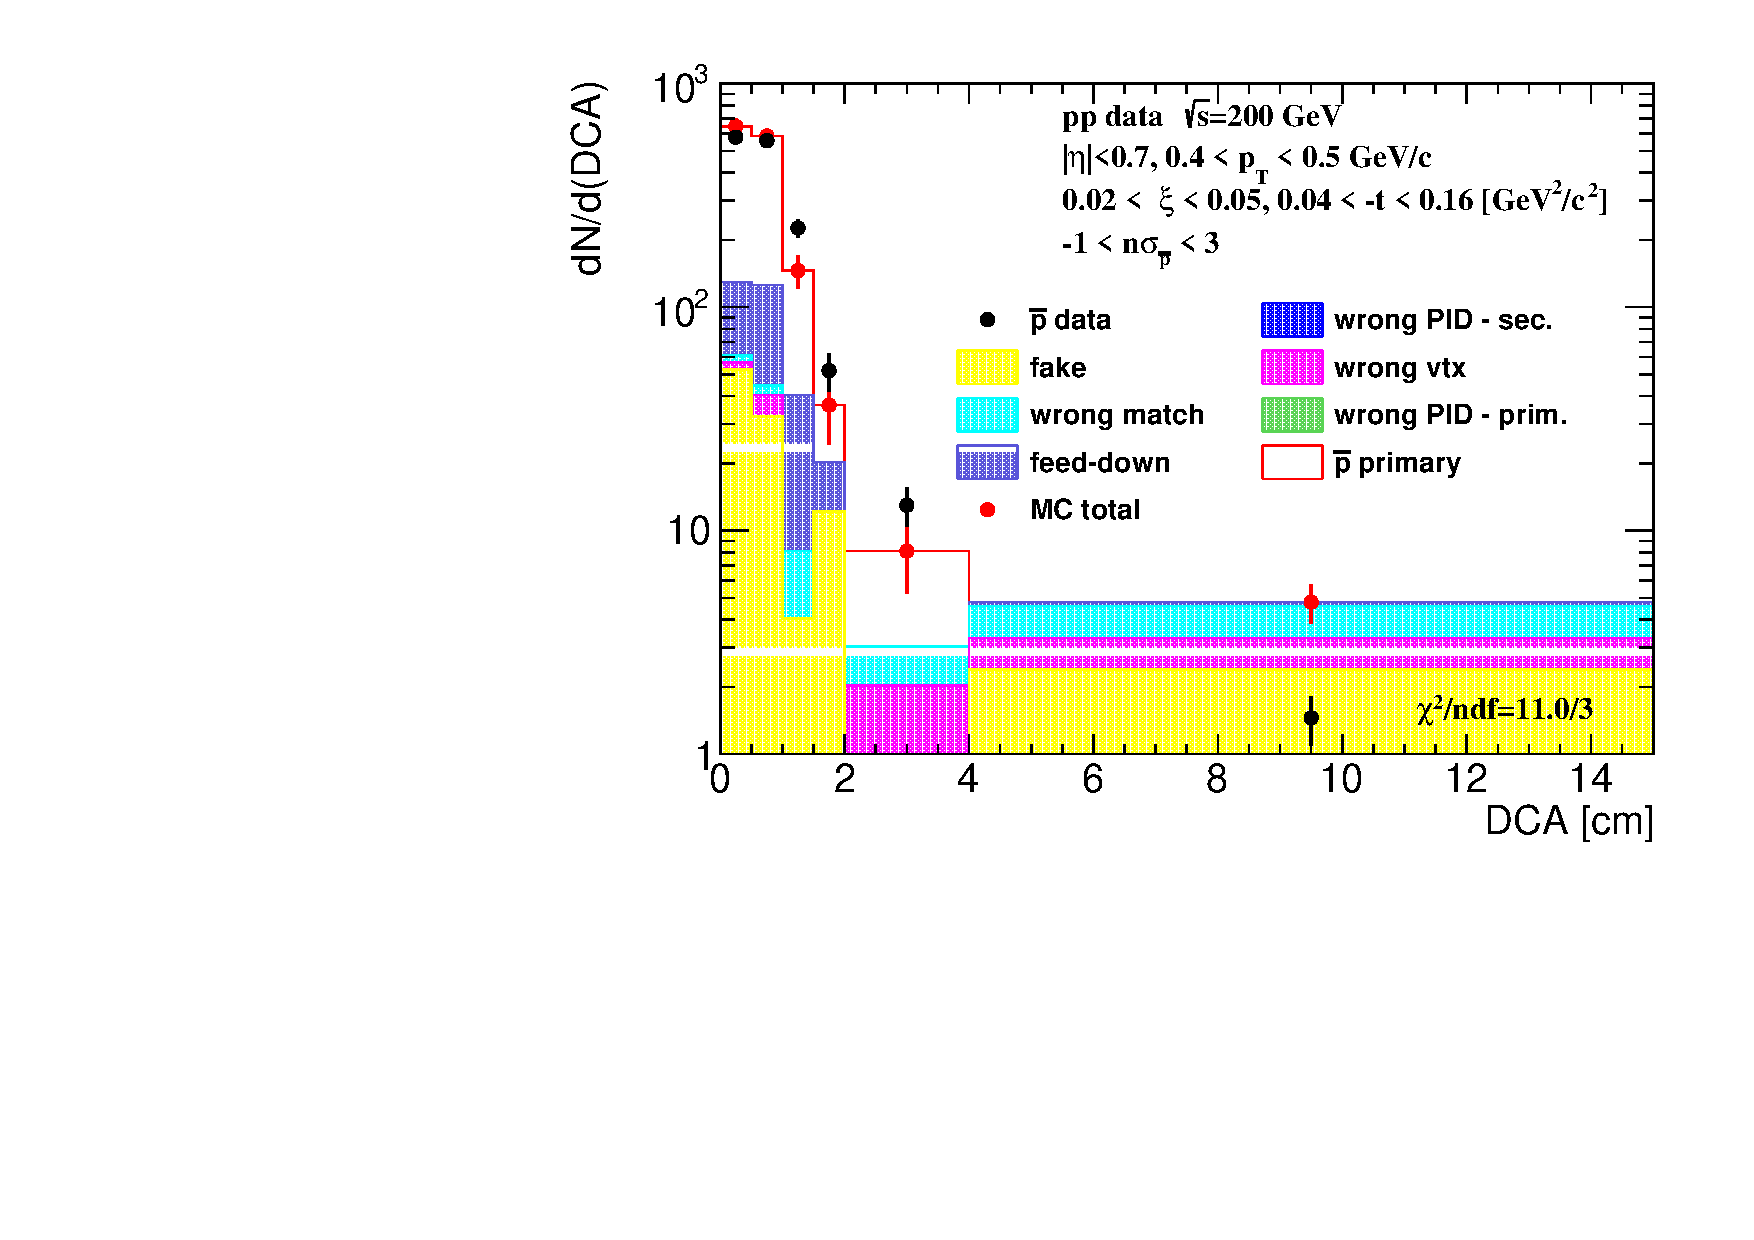
\includegraphics[width=\linewidth, page=1]{chapters/chrgSTAR/img/DCAproton/background_p_bar_0.pdf}
	\end{subfigure}
	\begin{subfigure}{.49\textwidth}
		\includegraphics[width=\linewidth, page=2]{chapters/chrgSTAR/img/DCAproton/background_p_bar_0.pdf}
	\end{subfigure}
	\begin{subfigure}{.49\textwidth}
		\includegraphics[width=\linewidth, page=3]{chapters/chrgSTAR/img/DCAproton/background_p_bar_0.pdf}
	\end{subfigure}
	\begin{subfigure}{.49\textwidth}
		\includegraphics[width=\linewidth, page=4]{chapters/chrgSTAR/img/DCAproton/background_p_bar_0.pdf}
	\end{subfigure}
	\caption{The $\textrm{DCA}$ distributions of antiprotons for $0.4<p_\textrm{T}<0.5$~GeV/c shown for one range of $0.02<\xi<0.05$ (log and linear scale in left and right column, respectively). The MC controbutions are shown as colour histograms. (top) Background enriched and (bottom) nominal samples were used.}
	\label{fig:bkg_proton_bar}
	%\vspace{-1cm}
\end{figure}

The fraction of the knock-out proton background in the signal region, $\textrm{DCA}<1.5$, was estimated from the nominal sample (Fig.~\ref{fig:bkg_proton}, bottom), where $\textrm{DCA}_{xy}$, $\textrm{DCA}_z$ and $d_0$ track cuts were applied and exactly one reconstructed vertex was required. The normalization of each MC contribution was kept the same as that estimated for the background enriched sample. Figure~\ref{fig:bkg_proton_fit} shows the knock-out proton background as a function of $p_\textrm{T}$ in three ranges of $\xi$. The following functional form was found to describe the
background protons:
\begin{equation}
f_{\textrm{bkg}}^{p}\left(p_\textrm{T}\right) = p_0\exp\left(p_1p_\textrm{T}\right)
\label{eq:protonBkgParametrization}
\end{equation}
where  $p_0$ and $p_1$ are  free parameters obtained from a~fit. 

The obtained fraction of knock-out background protons is approximately $20\%$ at $p_\textrm{T} = 0.45$ GeV/c
 and less than $10\%$ at $p_\textrm{T} = 1.0$~GeV/c.
 In PYTHIA~8 SD   predictions (also shown in~Fig.~\ref{fig:bkg_proton}), such fraction is much smaller  and equals to approximately $7\%$ at $p_\textrm{T} = 0.45$ GeV/c
 and about $5\%$ at $p_\textrm{T} = 1.0$~GeV/c. This may suggest that there are differences in the~amount of dead material in front of TPC  between data and simulation, which is consistent with the~studies presented in~\cite{supplementaryNote}.
 
 
 Figure~\ref{fig:bkg_proton_bar} shows the corresponding $\textrm{DCA}$ distributions with MC templates for antiprotons, where the background from knock-out particles is not present. Therefore, there was no need for any fit to be performed in this comparison. The MC templates  fairly well describe the $\textrm{DCA}$ distribution for both, protons, after tunning the~fraction of knock-out background to data, and antiprotons. %Additionally, there is a small $\left(<1\%\right)$ background  contribution, present for both particles, which also was taken into account and subtracted. It originates from reconstructed tracks which have the appropriate number of common hit points with true-level particle, but the~distance between them is too large, i.e. $\delta^2\left(\eta,\phi\right)>\left(0.15\right)^2$.
 

 \begin{figure}[h!]% \begin{wrapfigure}{r}{0.45\textwidth}
 	\centering
 	%\vspace{-20pt}
 	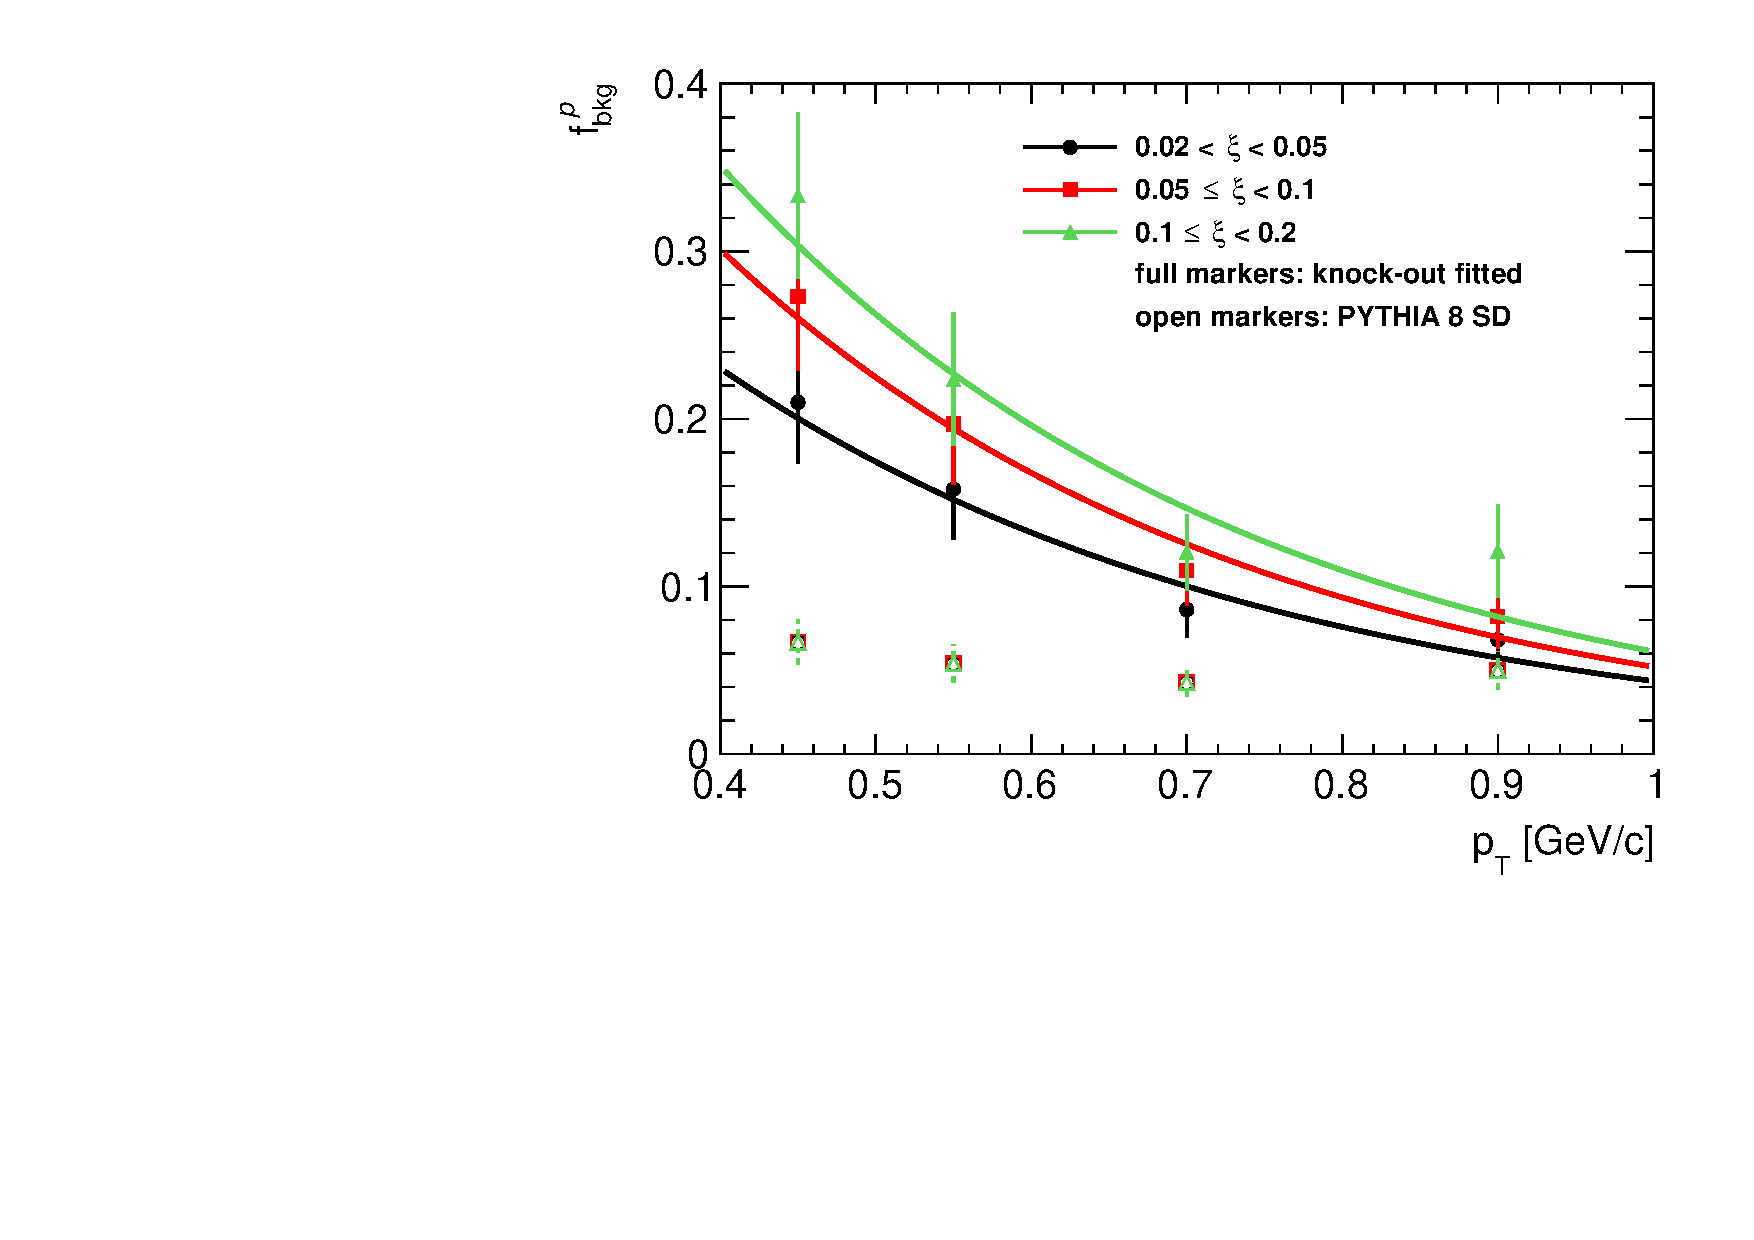
\includegraphics[width=0.8\linewidth, page=1]{chapters/chrgSTAR/img/DCAproton/bkg_p.pdf}
 	%\vspace{-20pt}
 	\caption{The fraction of knock-out proton background  as a function of $p_\textrm{T}$ in three ranges of $\xi$  with  fitted parametrizations. Full markers represent fitted knock-out background and open markers represent PYTHIA~8 SD predictions.}
 	%\vspace{-80pt}
 	\label{fig:bkg_proton_fit}
 \end{figure}

 
 \subsubsection{Systematic Uncertainty Related to Proton Background} 
The knock-out proton background estimation  introduces  systematic uncertainties. % which are added in quadrature. 
First, the normalization interval of the  knock-out   proton  background template in the background enriched sample was changed to $4<\textrm{DCA}<15$~cm. This introduced a relative systematic uncertainty of up to $30\%$ for $p_\textrm{T}\approx 0.9$~GeV/c. 

 \begin{figure}[h!]
 	\centering
 	\begin{subfigure}{.49\textwidth}
 		\includegraphics[width=\textwidth,page=1]{chapters/chrgSTAR/img/DCAproton/Ratio.pdf}
 	\end{subfigure}%\label{fig:protonBkgSystRatio}
 	\begin{subfigure}{.49\textwidth}
 		\includegraphics[width=\textwidth,page=1]{chapters/chrgSTAR/img/DCAproton/p_bkg.pdf}
 	\end{subfigure}
 	\begin{subfigure}{.49\textwidth}
 		\includegraphics[width=\textwidth,page=2]{chapters/chrgSTAR/img/DCAproton/p_bkg.pdf}
 	\end{subfigure}
 	\begin{subfigure}{.49\textwidth}
 		\includegraphics[width=\textwidth,page=3]{chapters/chrgSTAR/img/DCAproton/p_bkg.pdf}
 	\end{subfigure}
 	\caption{(top left) Data to MC ratio of  the  number of events in the background dominated region in three ranges of $\xi$ with fitted functional form given by Eq.~\eqref{eq:slopeBkgFit}. (top right and bottom) Components of the systematic uncertainty related to the  knock-out background protons contribution in three $\xi$ ranges. }
 	\label{fig:protonBkgSyst}
 	
 	\vspace{-1.5cm}
 \end{figure}

The  knock-out proton background contribution was  parameterized as  it is shown in  Eq.~\eqref{eq:protonBkgParametrization}. The systematic uncertainty related to the~parameterization procedure was estimated by varying the   parameters, $p_0$ and $p_1$, by their statistical uncertainties ($\pm1\sigma$).  As a result, a~relative systematic uncertainties of about $10\%$ were obtained.

Differences in the~shape of the~$\textrm{DCA}$ distribution between data and \ac{MC} can affect the~knock-out proton background estimation procedure. Figure~\ref{fig:protonBkgSyst} (top left) shows the data to MC ratio of  the  number of events in the background dominated region, $2<\textrm{DCA}<15$~cm. 
Since this region is used to estimate background normalization, and the shape of the $\textrm{DCA}$ distribution in the data differs from that observed in the simulation, the predicted background in the~$\textrm{DCA} <1.5$~cm region can change. Thus, the following functional form was used to estimate the slope between data and MC:
\begin{equation}
\frac{\textrm{data}}{\textrm{MC}}\left(\textrm{DCA}\right) = A(\textrm{DCA}-8.5)+B
\label{eq:slopeBkgFit}
\end{equation}
where $A$ (slope) and  $B$ are fit free parameters. Differences in slope between data and \ac{MC} were used to estimate how many
more background tracks would fit into the signal region and a systematic uncertainty, which varies up to $5\%$ for $0.02< \xi<0.05$, was introduced. 




All above components of the systematic uncertainty related to the knock-out proton background,  shown in Fig.~\ref{fig:protonBkgSyst}, are added in quadrature.
Those related to the~fit range and the~shape of the~proton background are symmetrized. Figure~\ref{fig:protonBkgSystSummary} shows the~fraction of knock-out proton background in three ranges of $\xi$ and the~total systematic uncertainty related to it.

\begin{figure}[h!]
	\centering
	\begin{subfigure}{.49\textwidth}
		\includegraphics[width=\textwidth,page=1]{chapters/chrgSTAR/img/DCAproton/p_bkg_summary.pdf}
	\end{subfigure}%\label{fig:protonBkgSystRatio}
	\begin{subfigure}{.49\textwidth}
		\includegraphics[width=\textwidth,page=2]{chapters/chrgSTAR/img/DCAproton/p_bkg_summary.pdf}
	\end{subfigure}
	\begin{subfigure}{.49\textwidth}
		\includegraphics[width=\textwidth,page=3]{chapters/chrgSTAR/img/DCAproton/p_bkg_summary.pdf}
	\end{subfigure}
	\begin{minipage}{.49\textwidth}
			\caption{The fraction of knock-out proton background  as a function of $p_\textrm{T}$   with  fitted parametrizations in three ranges of $\xi$: (top left) $0.02 < \xi < 0.05$, (top right) $0.05<\xi<0.1$ and (bottom) $0.1<\xi<0.2$. Gray bands represent total systematic uncertainties.}
			\label{fig:protonBkgSystSummary}
	\end{minipage}
\end{figure}


 
 \FloatBarrier
%background pion
\subsubsection{Pion Background}\label{section:star_background_pion}
The pion spectra are corrected for weak decays (mainly of $K^0_S$ and $\Lambda^0$), muon contribution and background from the   detector dead-material interactions. The pion decay muons can be identified as pions due to the similar masses. These contributions are obtained from PYTHIA~8 \ac{SD}. Figure~\ref{fig:bkg_pion} shows the background contribution to the pion spectra as a function of $p_\textrm{T}$ in three ranges of $\xi$, separately for $\pi^-$ and $\pi^+$.  Since there were   negligible differences  observed between these  three ranges of $\xi$, the background contribution was averaged over $\xi$. The following parametrization was found to describe it:
\begin{equation}
f_{\textrm{bkg}}^{\pi}\left(p_\textrm{T}\right)=a_0\exp(a_1p_\textrm{T})+a_2p_\textrm{T}^2+a_3p_\textrm{T}
\end{equation}
where $a_i$, $i=0,\dots, 3$ are free paramaters of the fitted function. 

The pion background contribution varies between $5\%$ at low-$p_\textrm{T}$  ($p_\textrm{T}=0.25$~GeV/c) and about $1\%$ at $p_\textrm{T}=1.0$~GeV/c for both negatively and positively charged pions. In addition, the~background was calculated from EPOS SD+SD$^\prime$ for the~full range of $\xi$. The~differences between PYTHIA~8 and EPOS are up to $1\%$ for $\pi^-$. 
\begin{figure}[htpb]
	\centering
	\begin{subfigure}{.49\textwidth}
		\includegraphics[width=\linewidth, page=1]{chapters/chrgSTAR/img/chargedBkg/bkg0max.pdf}
	\end{subfigure}
	\begin{subfigure}{.49\textwidth}
		\includegraphics[width=\linewidth, page=2]{chapters/chrgSTAR/img/chargedBkg/bkg0max.pdf}
	\end{subfigure}
	\caption{Pion background fraction as a function of $p_\textrm{T}$ calculated from PYTHIA~8 and shown separately for  (left) negatively  and (right)  positively charged pions in three ranges of $\xi$: (red) $0.02<\xi<0.05$,  (green) $0.05<\xi<0.1$, (blue) $0.1<\xi<0.2$.  (full black points) The pion background averaged over three ranges of $\xi$ with fitted parametrization is also shown. Open black points represent EPOS predictions for the full $\xi$ range.}
	\label{fig:bkg_pion}
\end{figure}

\FloatBarrier
